\documentclass[10pt,a4paper]{article}
\usepackage[utf8]{inputenc}
\usepackage{amsmath}
\usepackage{amsfonts}
\usepackage{amssymb}
\usepackage{graphicx}
\usepackage{epstopdf}
\usepackage{inputenc}
\usepackage[a4paper, total={150mm,250mm}]{geometry}
\usepackage{graphicx}
\usepackage{hyperref}
\usepackage[dvipsnames, table]{xcolor}
\usepackage{subcaption}
\usepackage{fancybox, graphicx}
\usepackage{tikz}
\usepackage{array}
\usepackage{ulem}
\usepackage{enumitem}
\usetikzlibrary{shadows}
\usepackage{listings}
\usepackage{bm}
\usepackage{lmodern,textcomp}
%\usepackage[english]{babel}


\makeatletter
\renewcommand\@biblabel[1]{\textbullet}
\makeatother
\newcommand{\question}[5]{
{#1}
\begin{enumerate}[label=\textbf{\alph*)}]
	\item {#2}
	\item {#3}
	\item {#4}
	\item {#5}
\end{enumerate}
}


\newcommand{\nline}{\\~\\}
\usepackage{tikz}
\hypersetup{
    colorlinks=true, %set true if you want colored links
	linkcolor=black,
    linktoc=all,     %set to all if you want both sections and subsections linked 
    urlcolor=blue
}
\title{{\Huge\textbf{USDE - Notes}
\\ \LARGE Unstructured Streaming and Data Engineering
\vspace{0.5em}
\\ \large \textbf{Professors}: Emanuele Della Valle - Marco Brambilla  \linebreak
\\ \small \textbf{Author}: Simone Staffa \linebreak

\vspace{5em}
\begin{figure}[h!]
 \hfill 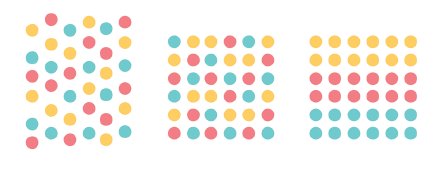
\includegraphics[width=300pt]{images/cover.png}\hspace*{\fill}
  \label{fig:polimi}
\end{figure}
}
\vspace{1em}
\small{
Released with Beerware License, Rev. 42 (https://spdx.org/licenses/Beerware.html) \linebreak
“As long as you retain this notice you can do whatever you want with this stuff. If we meet some day, and you think this stuff is worth it, you can buy me a beer in return”}
}
\begin{document}
\maketitle
\clearpage
\tableofcontents
\clearpage
\section{Introduction (Course motivation)}
\subsection{Data-driven Decision Making for Data-driven Organizations}
In many organizations decisions are made by "questionable" methodologies such as
\begin{itemize}
	\item \textbf{Hi}ghest \textbf{P}aid \textbf{P}erson \textbf{O}pinion (HiPPO): when Galileo tried to say that the earth cycles around the sun, the pope (the HiPPO) stated that heliocentrism was impossible.
	\item \textbf{Flipism}: all decisions are made by flipping a coin (randomly)
\end{itemize}
This could have been the right approach in the '70s... but in the Digital Era one can dream of data-driven organization, taking decisions using data.
\center{\textit{"\textbf{Decisions} no longer have to be made in the dark or based on gut instinct; they can be \textbf{based on evidence, experiments and more accurate forecasts}", McKinsey}}
\\ \vspace{0.5em}\raggedright
Data-driven organizations
\begin{itemize}
	\item \textbf{perform better}: the data shows where they can streamline their processes
	\item \textbf{are operationally more predictable}: data insights fuel current and future decision making
	\item \textbf{are more profitable}: constant improvements and better predictions help to outsmart the competition and improve innovation.
\end{itemize}
\subsection{Solving problems with Big Data, Data Science and ... Data Engineering}
\begin{figure}[h!]
 \hfill 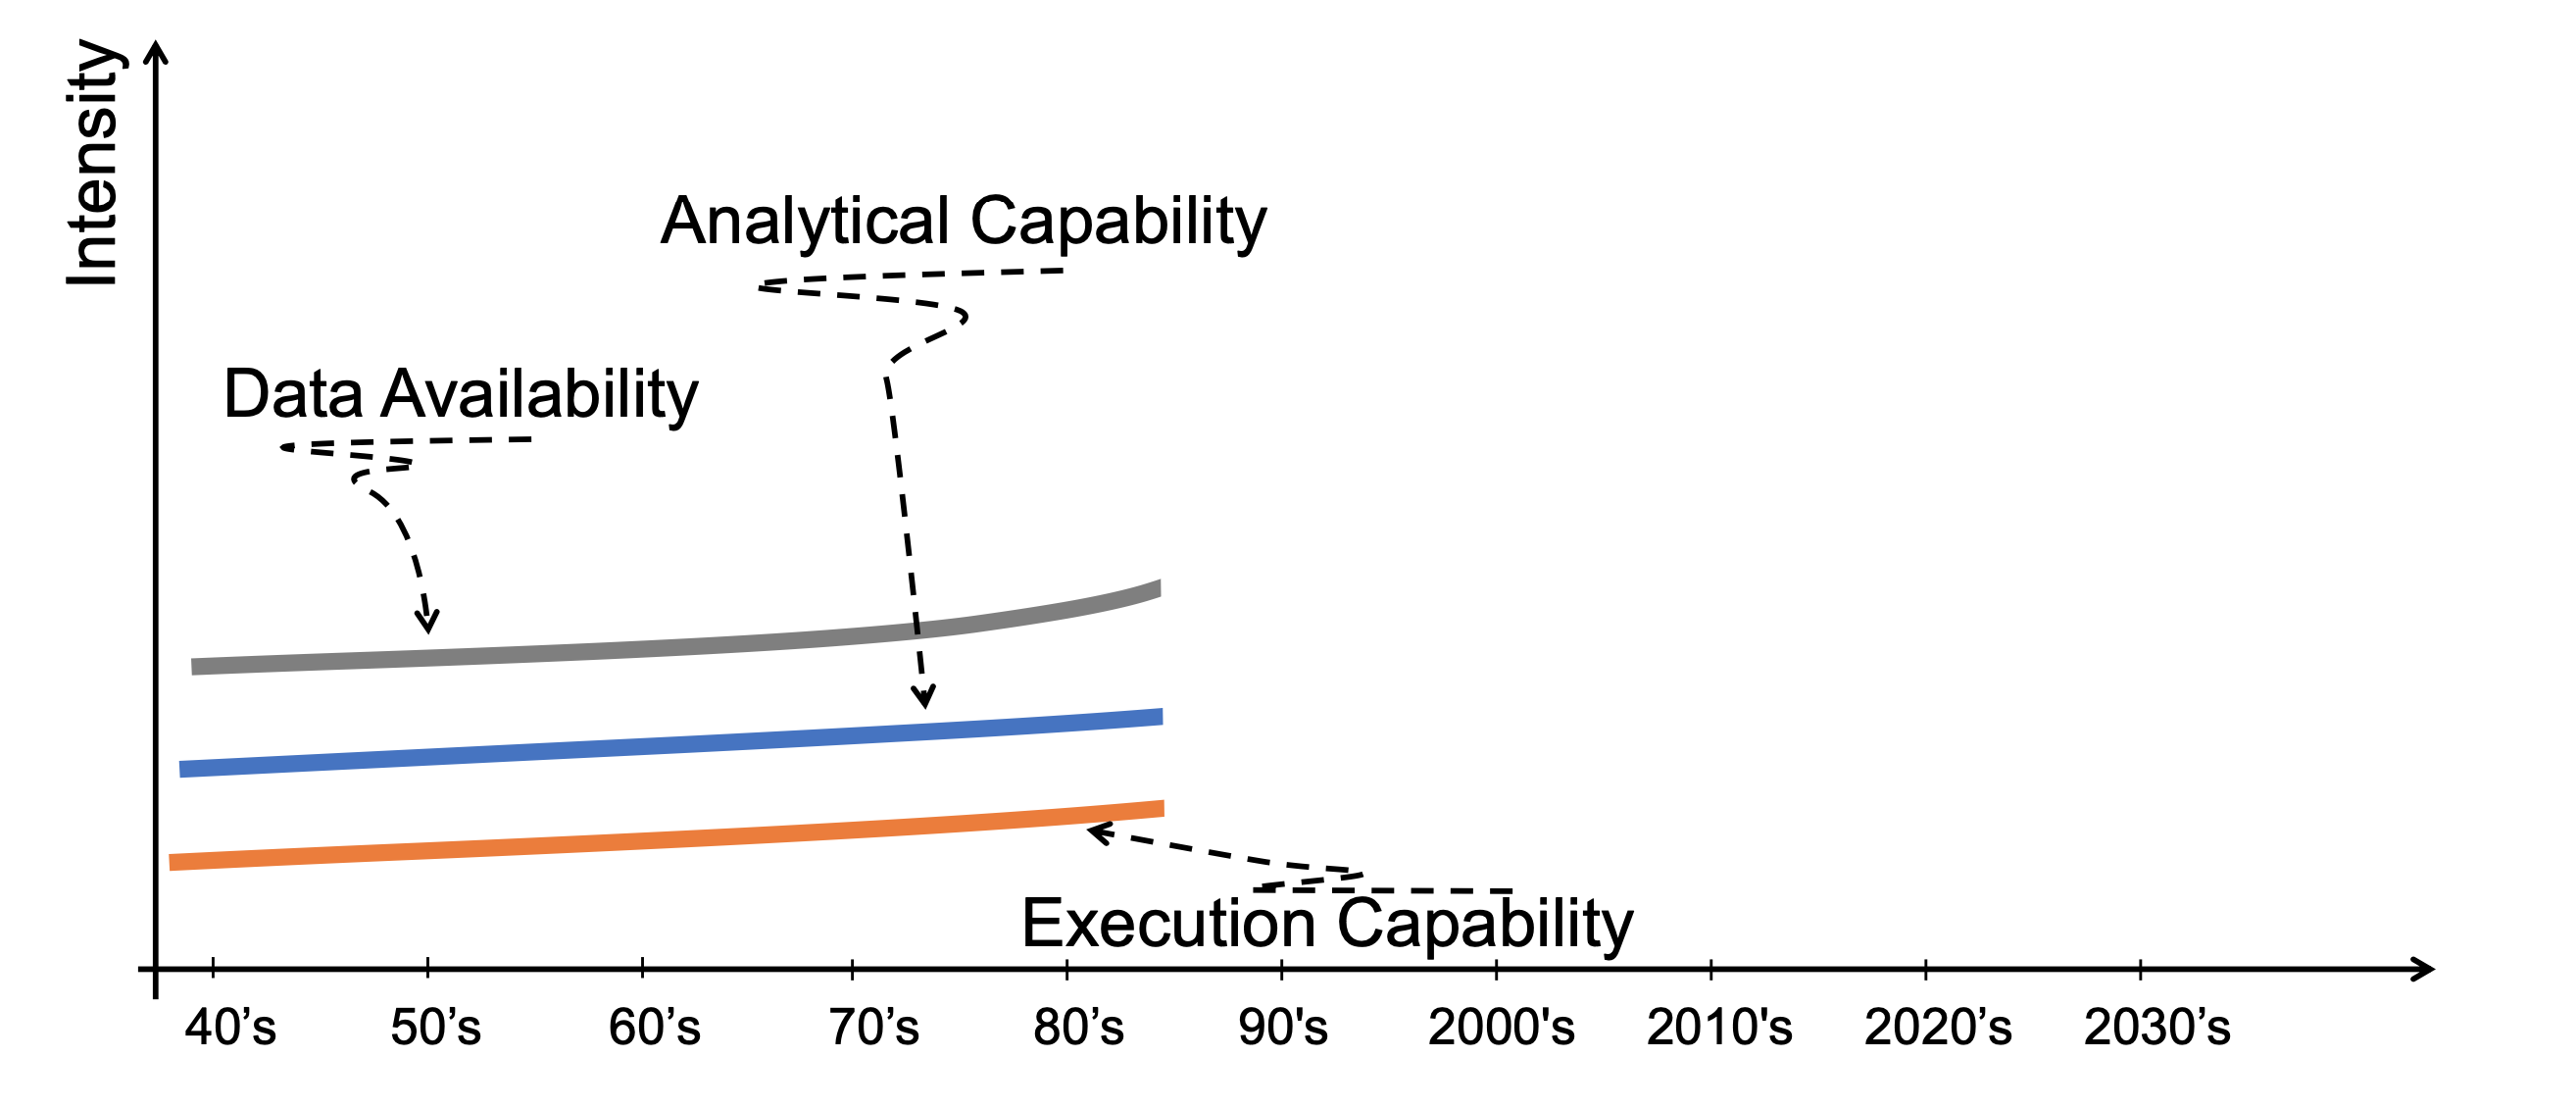
\includegraphics[width=300pt]{images/data-analysis.png}\hspace*{\fill}
  \label{fig:data-analysis}
  \caption{Up until '90s the data available was growing together with our analytical and execution capabilities.}
\end{figure}
\begin{figure}[h!]
 \hfill 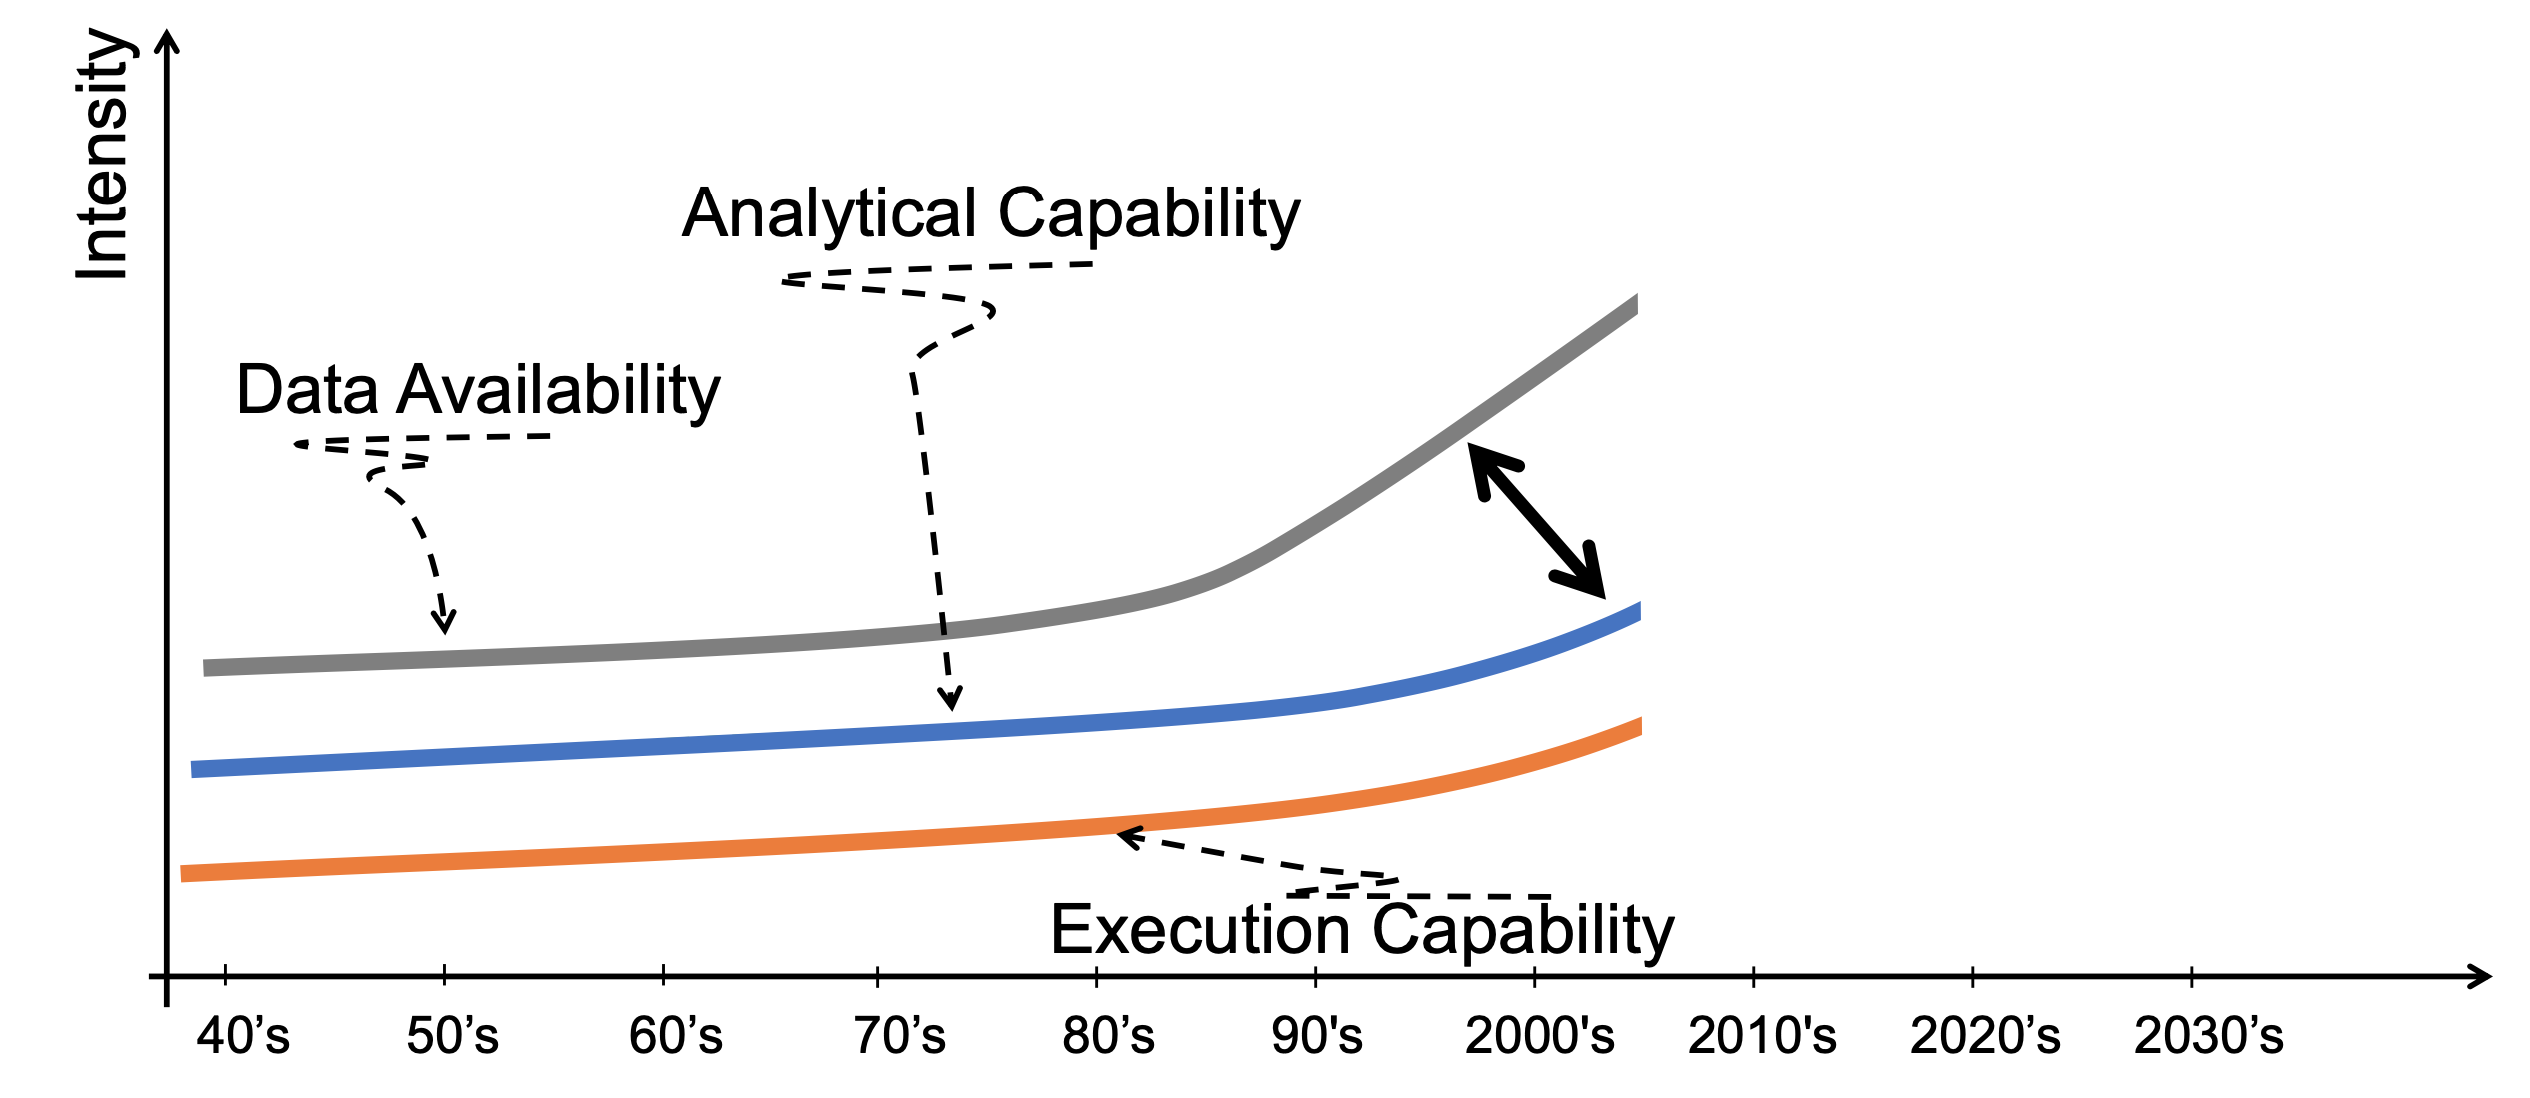
\includegraphics[width=300pt]{images/big-data.png}\hspace*{\fill}
  \label{fig:big-data}
  \caption{With the new millenium we have the appearence of Big Data. Data availability is growing fast and the digital revolution gap is growing.}
\end{figure}
\subsubsection{What's Big Data?}
Big data is a term that describes the large volume of data – both structured and unstructured – that inundates a business on a day-to-day basis. \\
IBM data scientists break big data into four dimensions: 
\begin{itemize}
	\item \textbf{Volume} (data at scale): volume is increasing, we have more and more data. Curiosity: in Italy is rare to find companies work with more than 20 Terabytes of data (only big customers)
	\item \textbf{Variety} (data in many form): structured, unstructured (or semi-structured e.g., graph), text, multimedia
	\item \textbf{Velocity} (data in motion): analysis of streaming data to enable decision within fractions of a second (real time decision and data analysis while data are coming). This is not a property of data but is specifically related to the kind of analysis we want to achieve.
	\item \textbf{Veracity} (data uncertainty): managing the reliability and predictability of inherently imprecise data type. This is not a property of data, it regards the quality of data. For 1 purpose the data are good, for another purpose the same data may not be good (or useful).
\end{itemize}
\begin{figure}[h!]
 \hfill 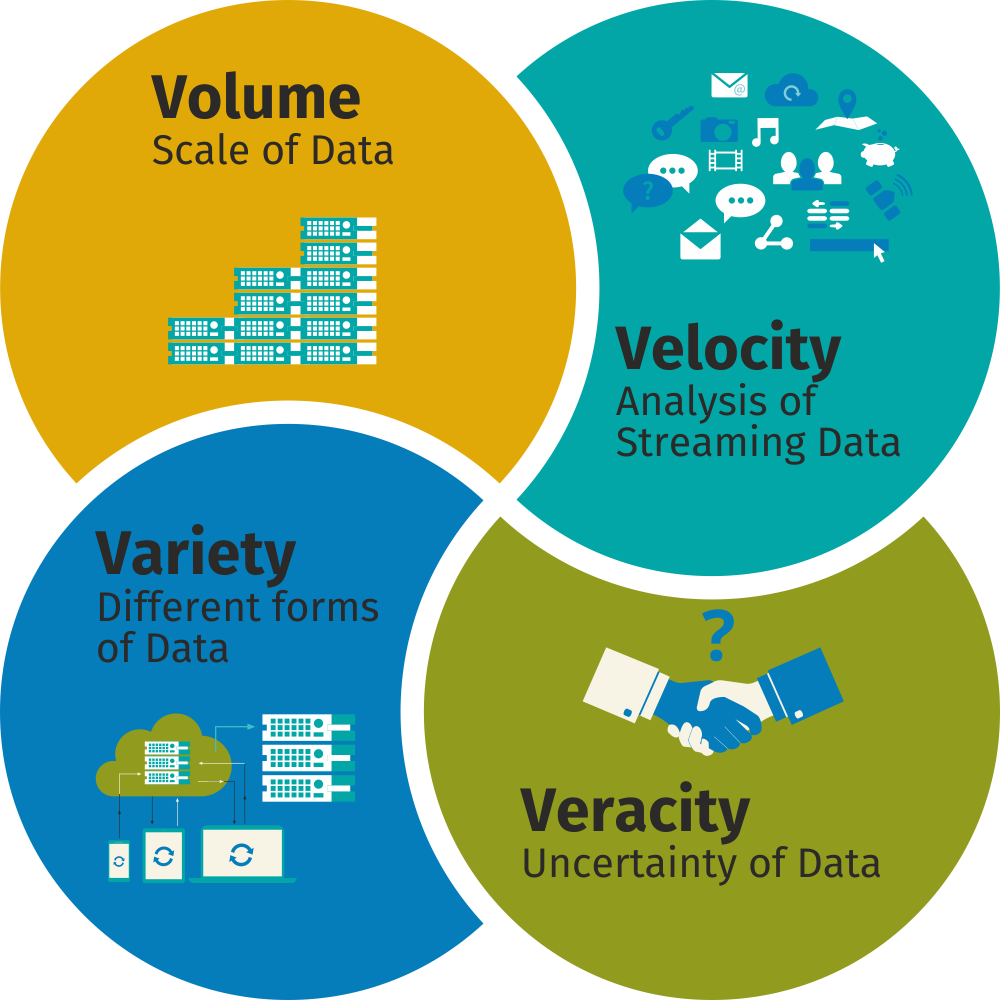
\includegraphics[width=200pt]{images/4v.png}\hspace*{\fill}
  \label{fig:4v}
  \caption{With the new millenium we have the appearence of Big Data. Data availability is growing fast and the digital revolution gap is growing.}
\end{figure}
Big Data techs are like "crude oil" that we have to:
\begin{itemize}
	\item Extract
	\item Transport in mega-tankers
	\item Ship through pipelines
	\item Store in massive silos
\end{itemize}
\begin{figure}[h!]
 \hfill 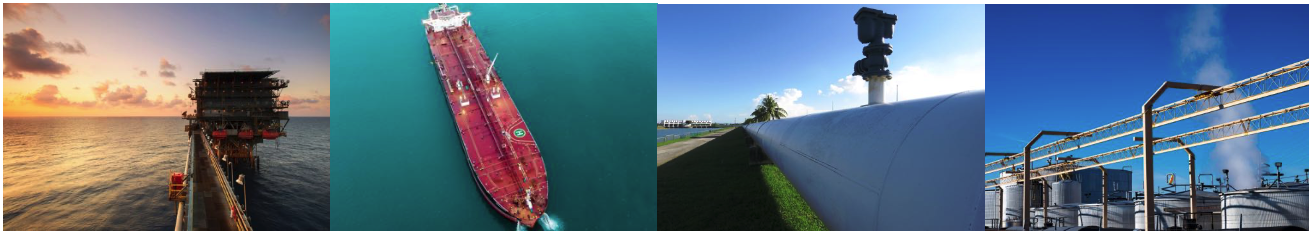
\includegraphics[width=300pt]{images/crude-oil.png}\hspace*{\fill}
  \label{fig:crude-oil}
\end{figure}
\subsubsection{What's Data Science}
The Science (and Art) of:
\begin{itemize}
	\item \textbf{Discovering} what we don’t know from data
	\item Obtaining \textbf{predictive, actionable insight} from data
	\item \textbf{Creating Data Products} that have business impact now
	\item \textbf{Communicating} relevant business stories from data
	\item \textbf{Building confidence} in decisions that drive business value
\end{itemize}
\textbf{Data scientists} are a new breed of analytical data expert who have the technical skills to solve complex problems – and the curiosity to explore what problems need to be solved. They’re part mathematician, part computer scientist and part trend-spotter. And, because they straddle both the business and IT worlds, they’re highly sought-after and well-paid.
\begin{figure}[h!]
 \hfill 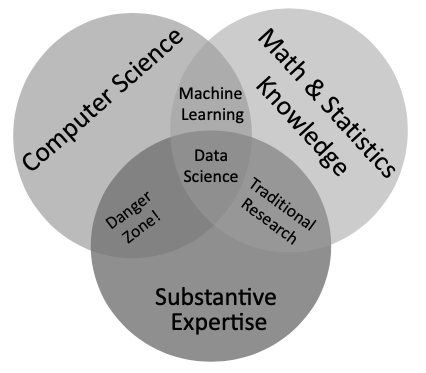
\includegraphics[width=200pt]{images/data-scientist.png}\hspace*{\fill}
  \label{fig:data-scientists}
\end{figure} \\
We distinguish \textbf{two cultures} of Statistical Modeling:
\begin{itemize}
	\item Data modeling (traditional research)
	\item Algorithmic modeling (more like machine learning)
\end{itemize}
\begin{figure}[h!]
 \hfill 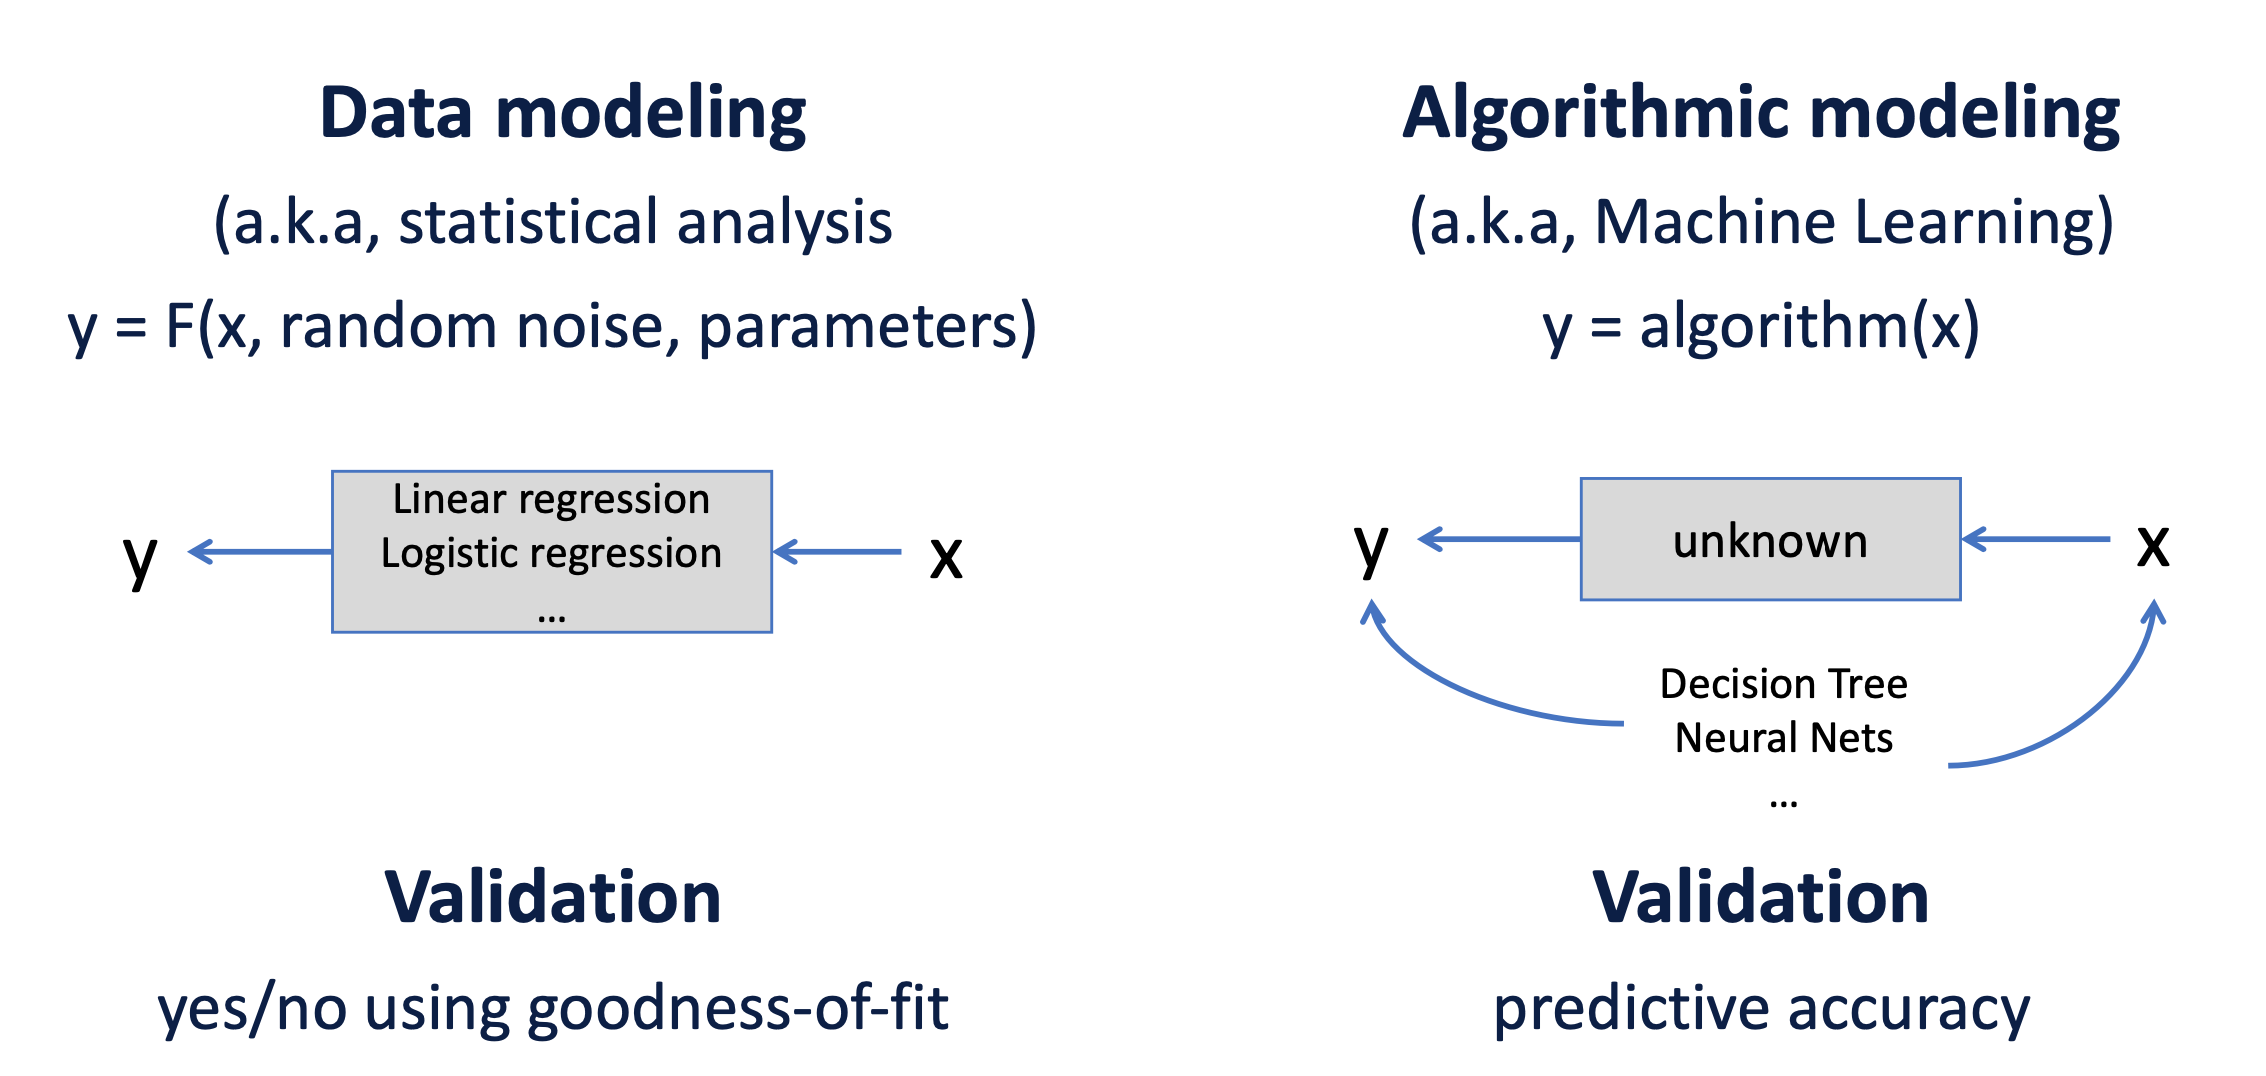
\includegraphics[width=250pt]{images/statistical-modeling.png}\hspace*{\fill}
  \label{fig:statistical-modeling}
\end{figure}
The algorithmic modeling culture starts with data and has two main goals:
\begin{itemize}
	\item Descriptions: describe how nature associates responses to inputs
	\item Predictions: predict response for future input variables
\end{itemize}
\pagebreak
\subsubsection{What's Data Engineering}
Following with the crude oil example, data engineers build "the refinery". 
\center{\textit{"A scientist can discover a new star, but he cannot make one. He would have to ask an engineer to do it for him."} - Gordon Lindsay Glegg} 
\\ \vspace{0.5em} \raggedright
A data engineer is a specialist that \textbf{maintain data and models available and usable} by others (i.e., Data Scientists and Business Analysts). According to Google: "A professional data engineer enables data-driven decision making by collecting, transforming, and publishing data. He should also be able to leverage, deploy, and continuously train pre-existing machine learning models." \\ \vspace{0.5em}
Data engineering purposes a paradigmatic shift, solving problems in new ways.
\begin{figure}[h!]
 \hfill 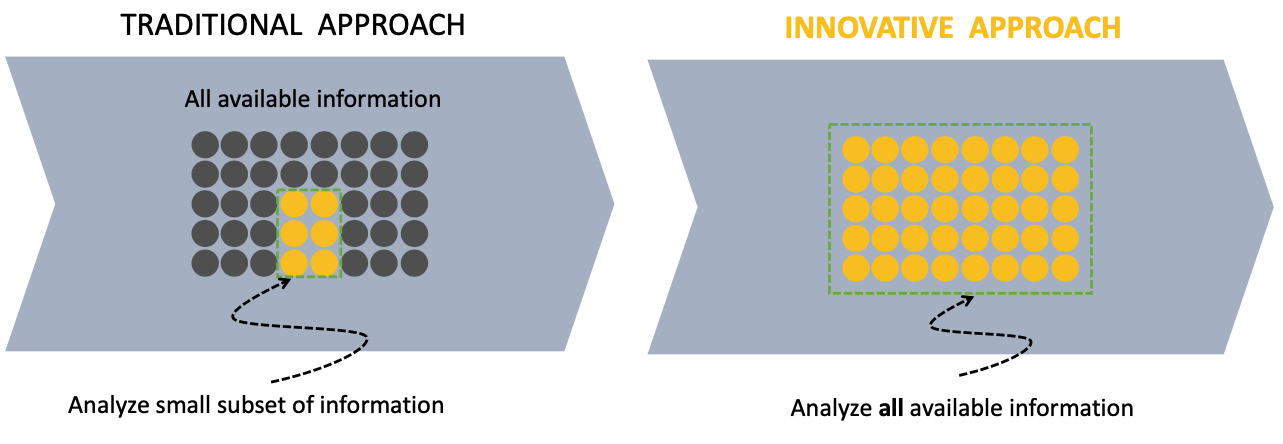
\includegraphics[width=250pt]{images/new-1.png}\hspace*{\fill}
  \label{fig:new1}
\end{figure}
\begin{figure}[h!]
 \hfill 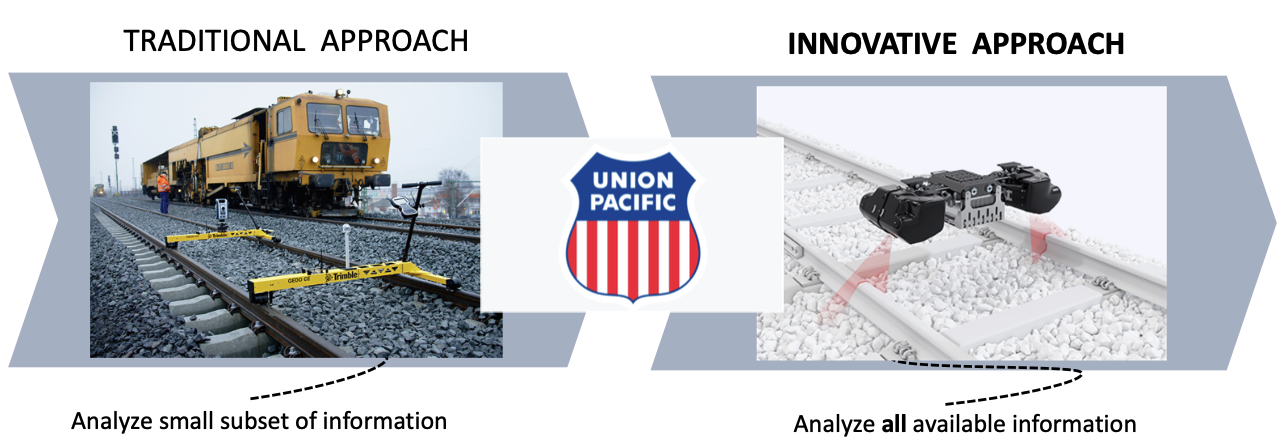
\includegraphics[width=250pt]{images/new-11.png}\hspace*{\fill}
  \label{fig:new11}
  \caption{Instead of looking for the perfect exact data, measure everything and \textbf{leverage more of the data being captured.} With a large enough dataset at some point we reach the same result (Central Limit Theorem).}
  \end{figure}
\begin{figure}[h!]
 \hfill 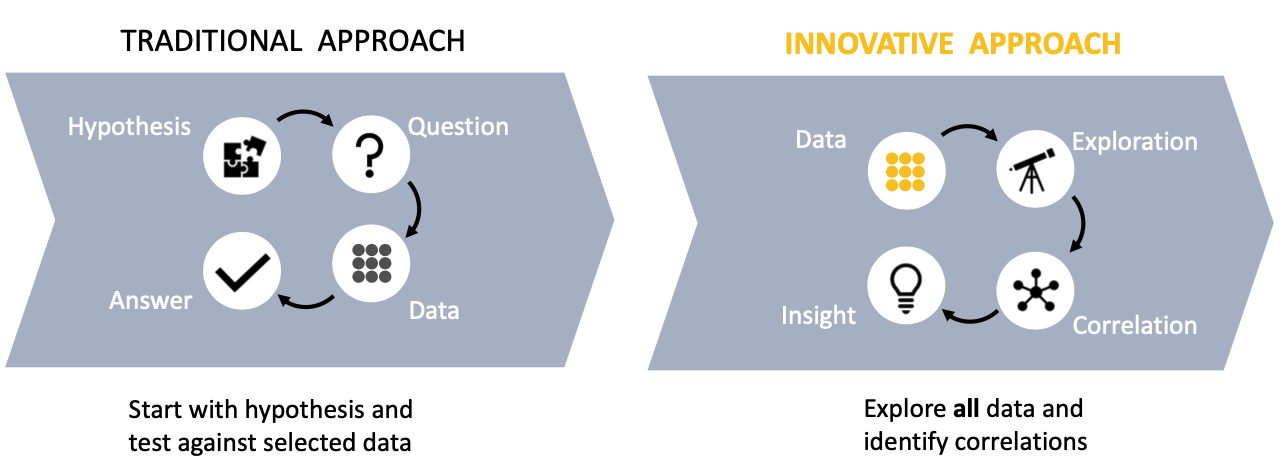
\includegraphics[width=250pt]{images/new-2.png}\hspace*{\fill}
  \label{fig:new2}
  \caption{\textbf{Data-driven exploration looking for correlation.} For instance, your butcher sells both pure meat and semi-prepared dishes because he knows that if you see the variety of products that he prepares and sells, you will probably notice something that you like!}
\end{figure}
 \\
  \pagebreak
\begin{figure}[h!]
 \hfill 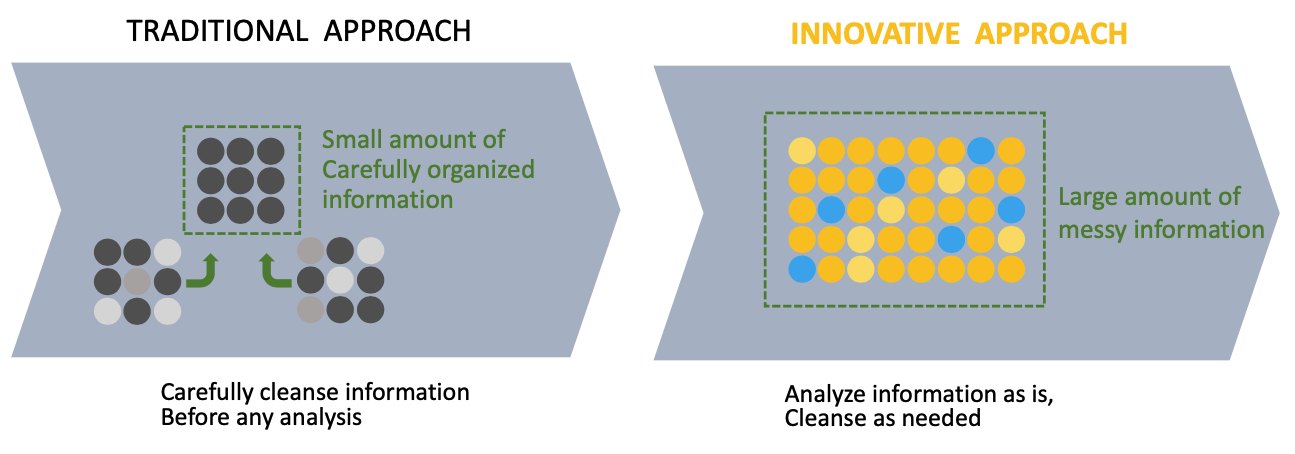
\includegraphics[width=250pt]{images/new-3.png}\hspace*{\fill}
  \label{fig:new3}
\end{figure}
\begin{figure}[h!]
 \hfill 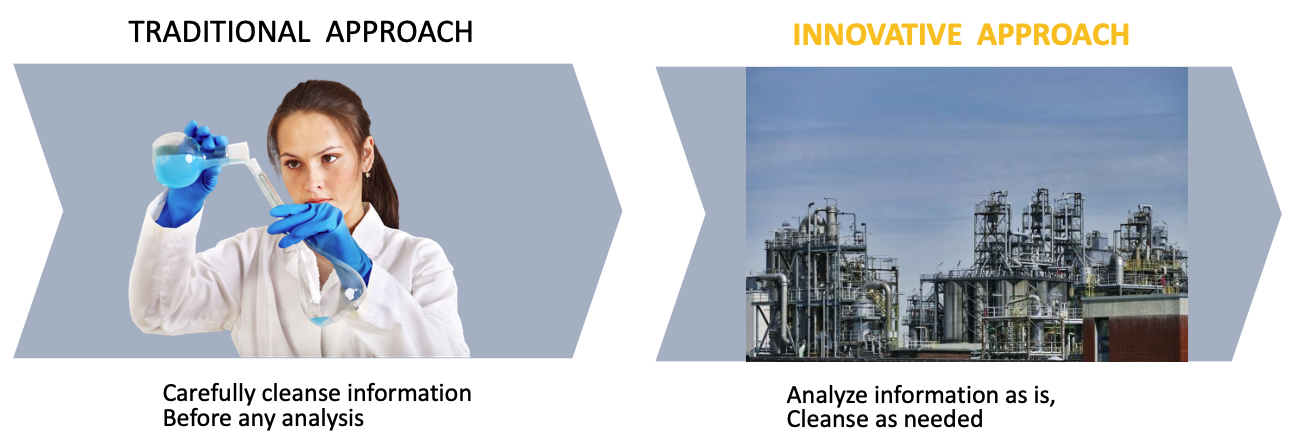
\includegraphics[width=250pt]{images/new-33.png}\hspace*{\fill}
  \label{fig:new33}
  \caption{\textbf{Reduce effort required to leverage data.} If you can do it by hand it is not said that you can do it automatically. Is hard to do things at scale.}
  \end{figure}
  \begin{figure}[h!]
 \hfill 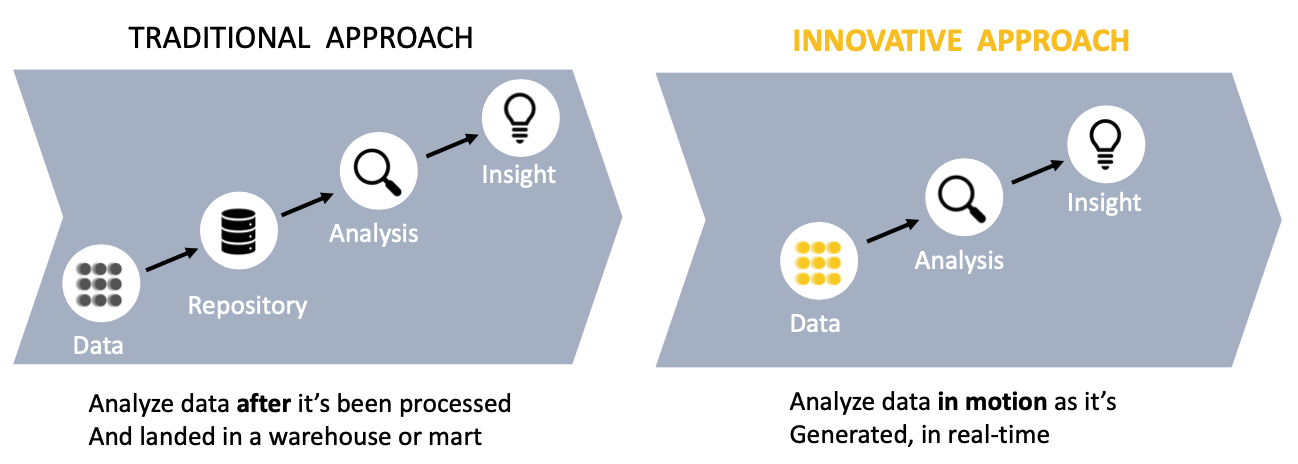
\includegraphics[width=250pt]{images/new-4.png}\hspace*{\fill}
  \label{fig:new4}
\end{figure}
\begin{figure}[h!]
 \hfill 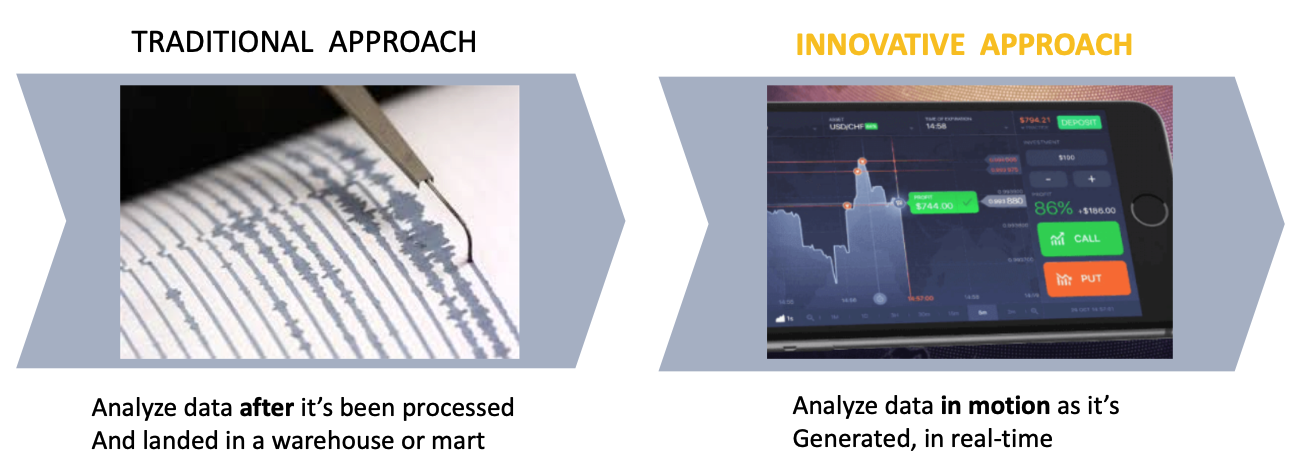
\includegraphics[width=250pt]{images/new-44.png}\hspace*{\fill}
  \label{fig:new44}
  \caption{\textbf{Leverage data as it is captured.}}
  \end{figure}
  The gap is closing thanks to Big Data, Data Science and ... Engineering.
  \begin{figure}[h!]
 \hfill 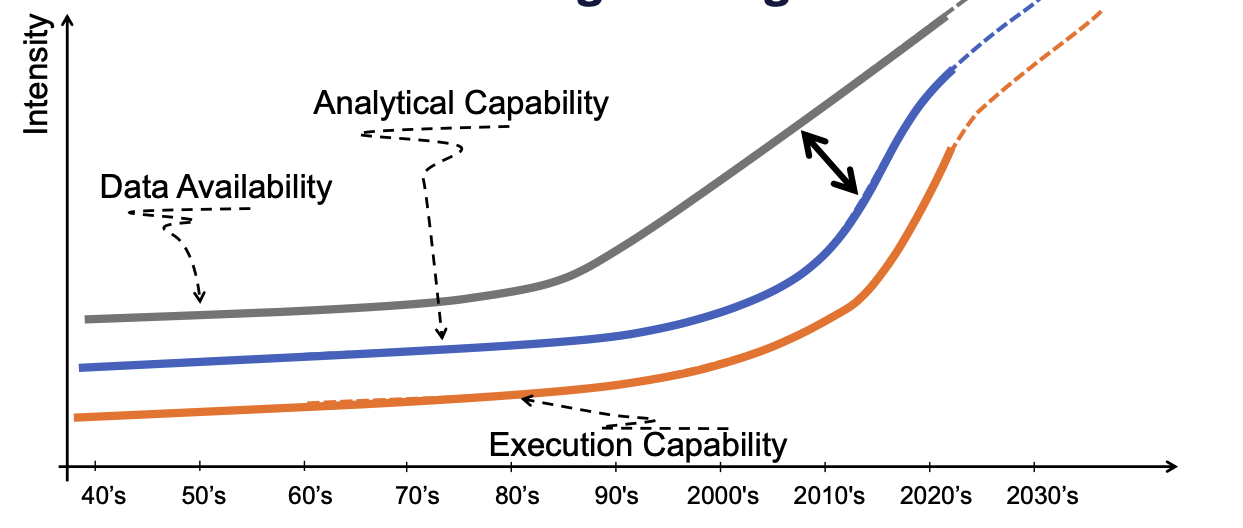
\includegraphics[width=250pt]{images/data-engineering-era.png}\hspace*{\fill}
  \label{fig:data-eng-era}
\end{figure}
\pagebreak
\section{No SQL Intro}
\subsection{Big Data Platforms: Architectures, Features and System}
\subsubsection{Big Data vs Traditional Data}
 \begin{figure}[h!]
 \hfill 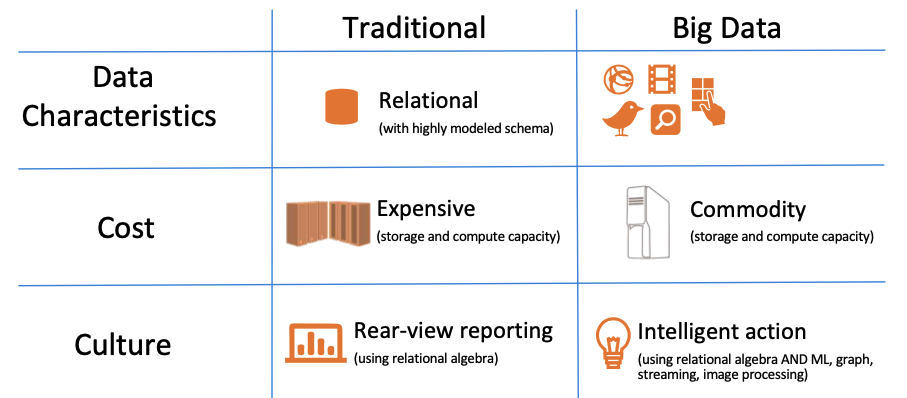
\includegraphics[width=300pt]{images/big-vs-traditional.png}\hspace*{\fill}
  \label{fig:big-vs-traditional}
  \caption{Big Data vs. Traditional Data}
\end{figure}
The first step towards Big Data and flexibility is to adopt a schema-less data storage. Indeed, we don't want to waste time designing complex and fixed schema.
\begin{itemize}
	\item Aggregate-based: key-value, big-table, column-based, document-based
	\item Relationship-based: graph dbs are better than relational!
\end{itemize}
Even in this context we see a paradigmatic shift introduced by Big Data. From \textbf{schema on write} to \textbf{schema-on-read}.
\begin{figure}[h!]
\centering
\begin{minipage}{.5\textwidth}
  \centering
  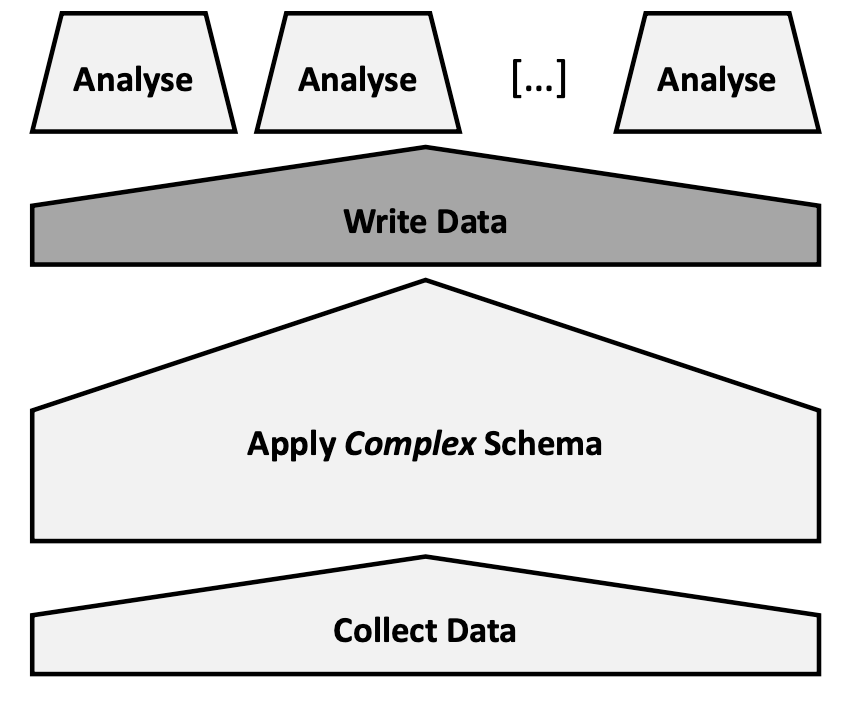
\includegraphics[width=.8\linewidth]{images/schema-on-write}
  \captionof{figure}{\textbf{Schema-on-write}: the rigid and traditional strategy (relational data) in which a complex schema is applied after a long lasting discussing. Here we collect the data from different sources, ensuring that it is compatible with our schema and then we make analysis on that.}
  \label{fig:sow}
\end{minipage}%
\begin{minipage}{.5\textwidth}
  \centering
  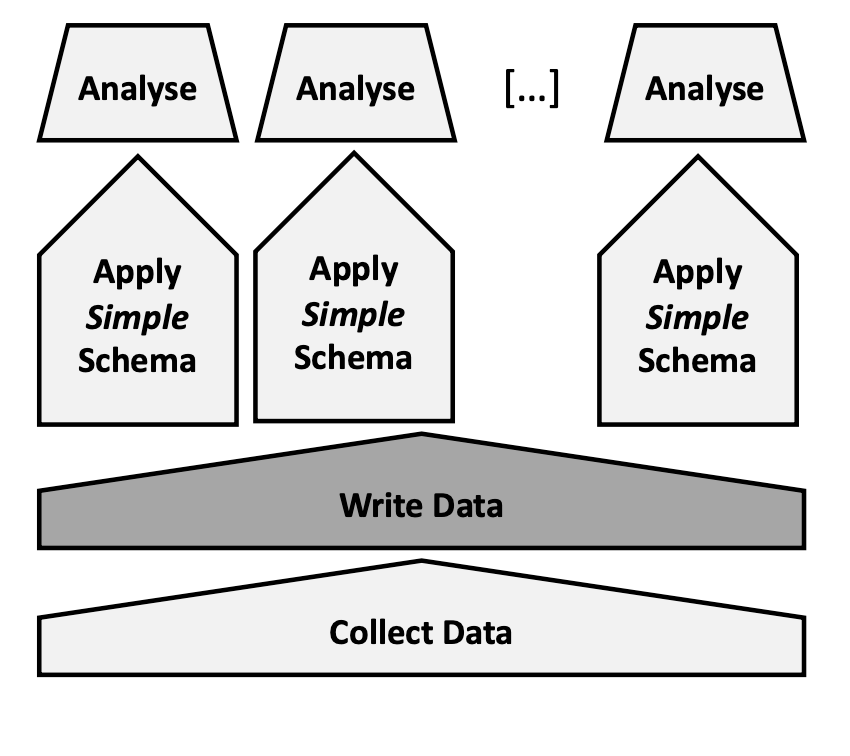
\includegraphics[width=.8\linewidth]{images/schema-on-read}
  \captionof{figure}{\textbf{Schema-on-read}: schema-less approach (document-based data) in which we collect and load data first and ask questions/queries later. All data are kept and the minimal schema for an analysis is applied only when needed. New analysis can then be introduced in any point in time.}
  \label{fig:sor}
\end{minipage}
\end{figure}
\pagebreak
\subsubsection{The Concept of Data Lake}
A Data Lake is a repository in which we store all the possible data that we need in our business. These raw data can be structured or unstructured, without any specific organization and they are there ready to be analyzed when needed. Indeed, there is a specific process that characterized the flow of Big Data into the Data Lake and the various transformation that are applied before analysis and visualization.
\begin{figure}[h!]
\centering
\begin{minipage}{.5\textwidth}
  \centering
  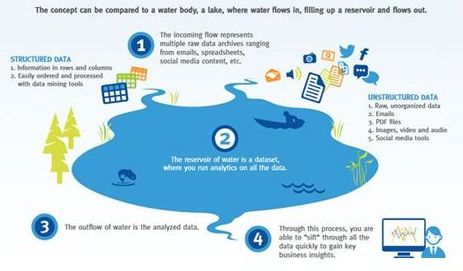
\includegraphics[width=.9\linewidth]{images/data-lake}
  \captionof{figure}{Data lake}
  \label{fig:data-lake}
\end{minipage}%
\begin{minipage}{.5\textwidth}
  \centering
  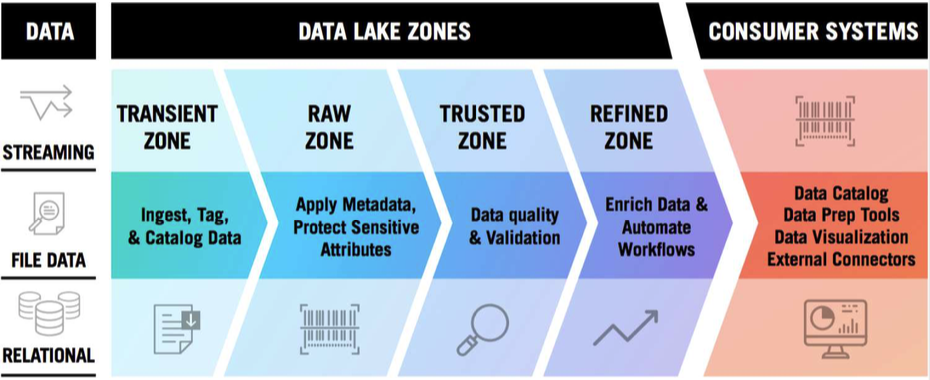
\includegraphics[width=.9\linewidth]{images/data-lake-process}
  \captionof{figure}{Data Lake in process}
  \label{fig:data-lake-process}
\end{minipage}
\end{figure}  \\
\textbf{Data Ingestion} is the process of importing, transferring and loading data for storage and later use. It involves loading data from a variety of sources. It can involve altering and modification of individual files to fit into a format that optimizes the storage. For instance, in Big Data small files are concatenated to form files of 100s of MBs and large files are broken down in files of 100s of MBs. \\
\textbf{Data Wrangling}: the process of cleansing "raw" data and transforming raw it into data that can be analysed to generate valid actionable insight. It includes understanding, cleansing, augmenting and shaping data. The results is data in the best format (e.g., columnar) for the analysis to perform.
\begin{figure}[h!]
 \hfill 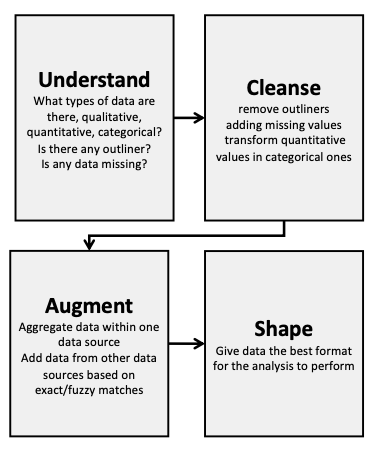
\includegraphics[width=200pt]{images/data-wrangling.png}\hspace*{\fill}
  \label{fig:data-wrangling}
  \caption{Data Wrangling}
\end{figure}
\pagebreak
\subsubsection{Scalability}
Adding data to a system may degrade its performances.
\begin{itemize}
	\item \textbf{"Traditional" SQL system scale vertically}: when the machine, where the SQL system runs, no longer performs as required, the solution is to \textbf{buy a better machine} (with more RAM, more cores and more disk).
	\item \textbf{Big Data solutions scale horizontally}: when the machines, where the big data solution runs, no longer performs as required, the solution is \textbf{to add another machine.}
\end{itemize}
\begin{figure}[h!]
\centering
\begin{minipage}{.5\textwidth}
  \centering
   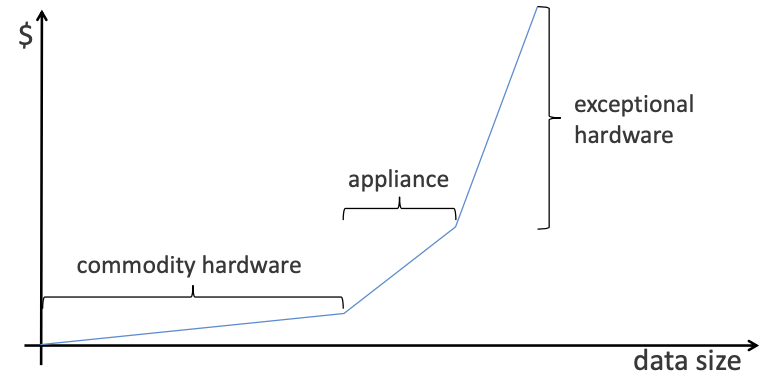
\includegraphics[width=.9\linewidth]{images/vertical-scalability}
  \captionof{figure}{Vertical Scalability}
  \label{fig:vertical}
\end{minipage}%
\begin{minipage}{.5\textwidth}
  \centering
  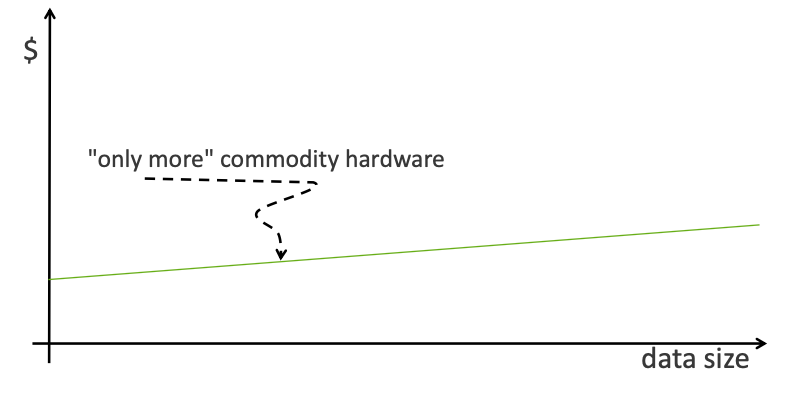
\includegraphics[width=.9\linewidth]{images/horizontal-scalability}
  \captionof{figure}{Horizontal Scalability}
  \label{fig:horizontal}
\end{minipage}
\end{figure} 
\begin{figure}[h!]
 \hfill 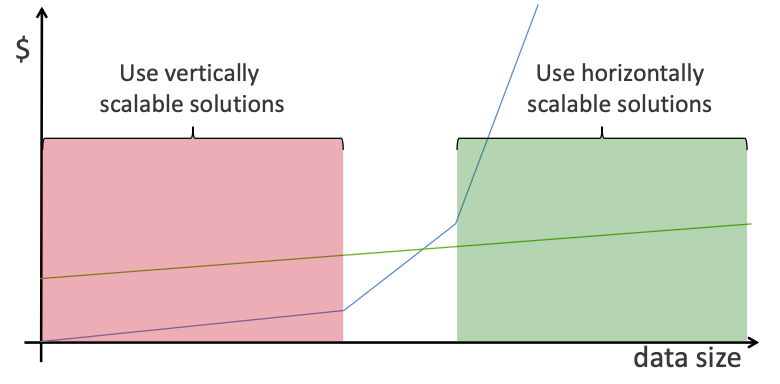
\includegraphics[width=200pt]{images/vertical-vs-horizontal.png}\hspace*{\fill}
  \label{fig:vertical-vs-horizontal}
  \caption{Vertical (Exponential) vs Horizontal (Linear) growth}
\end{figure}

\begin{figure}[h!]
\centering
\begin{minipage}{.5\textwidth}
  \centering
   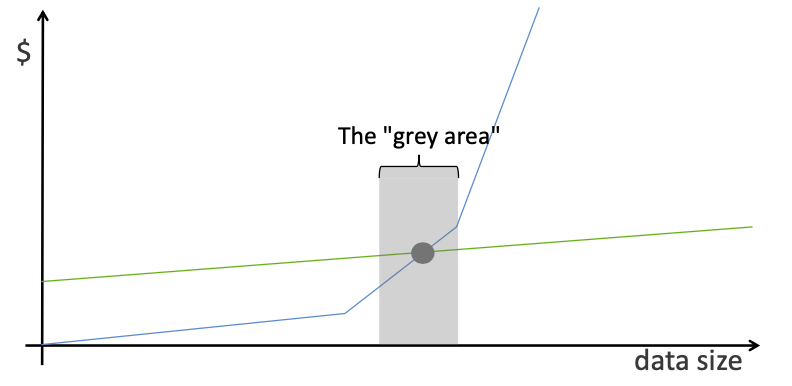
\includegraphics[width=.9\linewidth]{images/grey-area}
  \captionof{figure}{The space within vertical (blue) and horizontal (red) scalable solution. On the left we see an high price gap between the blue and the red line for which the preferred solution is the vertical scalability. On the right is the contrary: the price is growing faster on the blue line while the horizontal scalable solution price is growing linearly.}
  \label{fig:grey-area}
\end{minipage}%
\begin{minipage}{.5\textwidth}
  \centering
  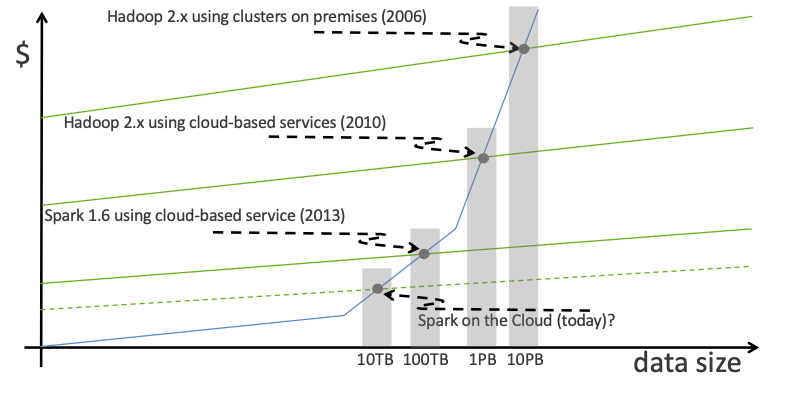
\includegraphics[width=.9\linewidth]{images/grey-area-in-time}
  \captionof{figure}{The grey area moves in time. As a result, we can see that horizontal scalability now makes sense when we have to deal with 10TB of data.}
  \label{fig:grey-area-in-time}
\end{minipage}
\end{figure} 
\pagebreak
\subsection{ACID vs. BASE and SQL vs. NoSQL}
\subsubsection{Transactional Properties}
\uline{Definition of Transaction}: An elementary unit of work performed by an application. Each transaction is encapsulated within two commands: \textbf{begin transaction} (bot) and \textbf{end transaction} (eot).
\\ Within a transaction of the commands below is executed \textit{exactly once}:
\textcolor{red}{commit work} (commit) and \textcolor{red}{rollback work} (abort). \\
A \textcolor{red}{Transactional System} (OLTP) is a system capable of providing the definition and execution of transactions on behalf of multiple, concurrent applications.
\begin{figure}[h!]
 \hfill 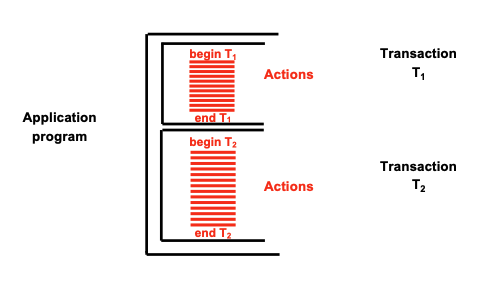
\includegraphics[width=200pt]{images/transactions.png}\hspace*{\fill}
  \label{fig:transactions}
  \caption{Application and Transactions}
\end{figure}
\begin{figure}[h!]
\centering
\begin{minipage}{.5\textwidth}
  \centering
   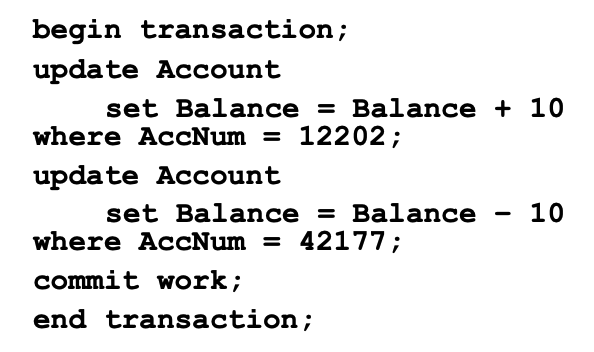
\includegraphics[width=.7\linewidth]{images/transaction-ex}
  \captionof{figure}{Transaction example}
  \label{fig:t1}
\end{minipage}%
\begin{minipage}{.5\textwidth}
  \centering
  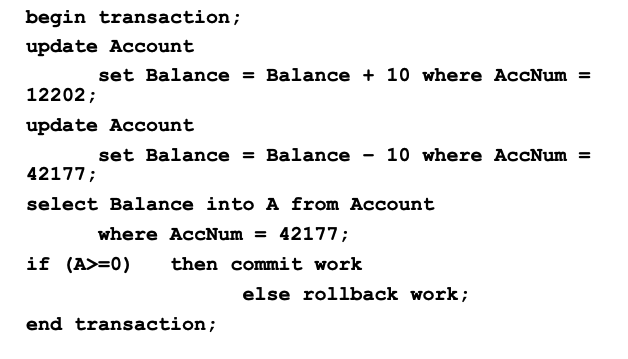
\includegraphics[width=.7\linewidth]{images/transaction-ex2}
  \captionof{figure}{Another Transaction example with rollback}
  \label{fig:t2}
\end{minipage}
\end{figure} 
\paragraph{ACID Properties of Transactions}
A transaction is a unit of work enjoying the following properties:
\begin{itemize}
	\item \textbf{Atomicity}: a transaction is an atomic transformation from the initial state to the final state. Three possible behaviors:
	\begin{itemize}
		\item Commit work: SUCCESS
		\item Rollback work or error prior to commit: UNDO
		\item Fault after commit: REDO
	\end{itemize}
	\textcolor{red}{Abort-rollback restart} and \textcolor{red}{Commit protocols}
	\item \textbf{Consistency}: the transaction satisfies the integrity of constraints on data. As a consequence, if the initial state is consistent, then the final state is also consistent. \textcolor{red}{Integrity checking of DBMS}
	\item \textbf{Isolation}: a transaction is not affected by the behavior of other, concurrent transactions. As a consequence, its intermediate states are not exposed and the "domino effect" is avoided. \textcolor{red}{Concurrency control}
	\item \textbf{Durability}: the effect of a transaction that has successfully committed will last "forever" independently of any system fault. \textcolor{red}{Recovery management}
\end{itemize}
These properties characterizes relational DBMS and for this reason such systems offer very expensive and rigid solutions.
\subsubsection{CAP Theorem}
It is impossible for a \uline{distributed computer system} to simultaneously provide all three of the following guarantees:
\begin{itemize}
	\item \textbf{Consistency}: all nodes see the same data at the same time
	\item \textbf{Availability}: node failures do not prevent other survivors from continuing to operate (a guarantee that every request receives a response about whether it succeeded or failed)
	\item \textbf{Partition tolerance}: the system continues to operate despite arbitrary partitioning due to network failures (e.g., message loss)
\end{itemize}
A distributed system can satisfy any two of these guarantees at the same time but not all three. \\ 
In a distributed system, a network (of networks) is inevitable (by definition). We can't avoid to deal with partition tolerance, we need to cover that. Indeed. Failures can, and will, occur to a networked system. Then, the only option left is choosing between \textbf{C}onsistency and \textbf{A}vailability. This because CA doesn't make any sense, because is what traditional centralized database are guaranteeing. \\
We have two solutions:
\begin{itemize}
	\item AP: a partitioned node returns
	\begin{itemize}
		\item a correct value, if in a consistent state;
		\item a timeout error or an error, otherwise;
		\item e.g., DynamoDB, CouchDB, and Cassandra
	\end{itemize}
	\item CP: a partitioned note returns the most recent version of the data, which could be stale
	\begin{itemize}
		\item e.g., MongoDB, Redis, AppFabric Caching and MemcacheDB
	\end{itemize}
\end{itemize}
By the way, Consistency and Availability should not necessarily be guaranteed in a mutually exclusive manner, but possibly by partial accomodation of both. We need to do some trade-off analyses.
\begin{figure}[h!]
\centering
\begin{subfigure}{.5\textwidth}
  \centering
  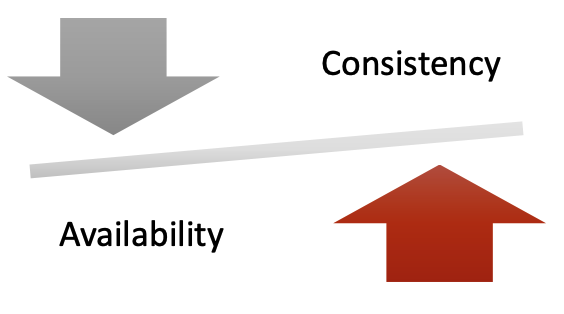
\includegraphics[width=.5\linewidth]{images/availability-vs-consistency}
  \caption{\textbf{Consistency vs Availability}}
  \label{fig:ca}
\end{subfigure}%
\begin{subfigure}{.5\textwidth}
  \centering
  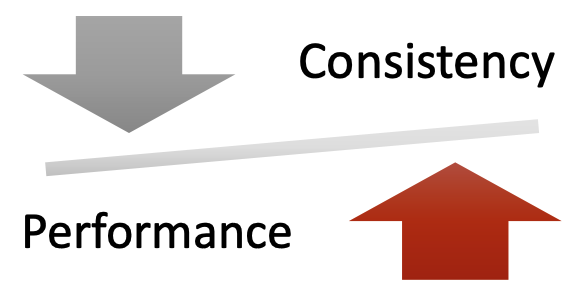
\includegraphics[width=.5\linewidth]{images/performance-vs-consistency}
  \caption{\textbf{Consistency vs Performance}}
  \label{fig:cp}
\end{subfigure}
\caption{We need to choose between consistency and availability. According to the use case scenario, we can choose which one to favour. For example, \uline{consistency should be preferred in banking applications}, where the transactions of money should be carefully saved and stored in a rigid flow to allow the correct functioning of the system. While almost \uline{all the social media apps or streaming platforms may concentrate on availability} since if some data in the communication is lost or some user content are not presented in the latest version, the app can continue providing the service without creating any big issues to the user. Talking about \uline{performance}, high consistency usually results in low performance while high performance results in low consistency.}
\label{fig:cap}
\end{figure}
\begin{figure}[h!]
 \hfill 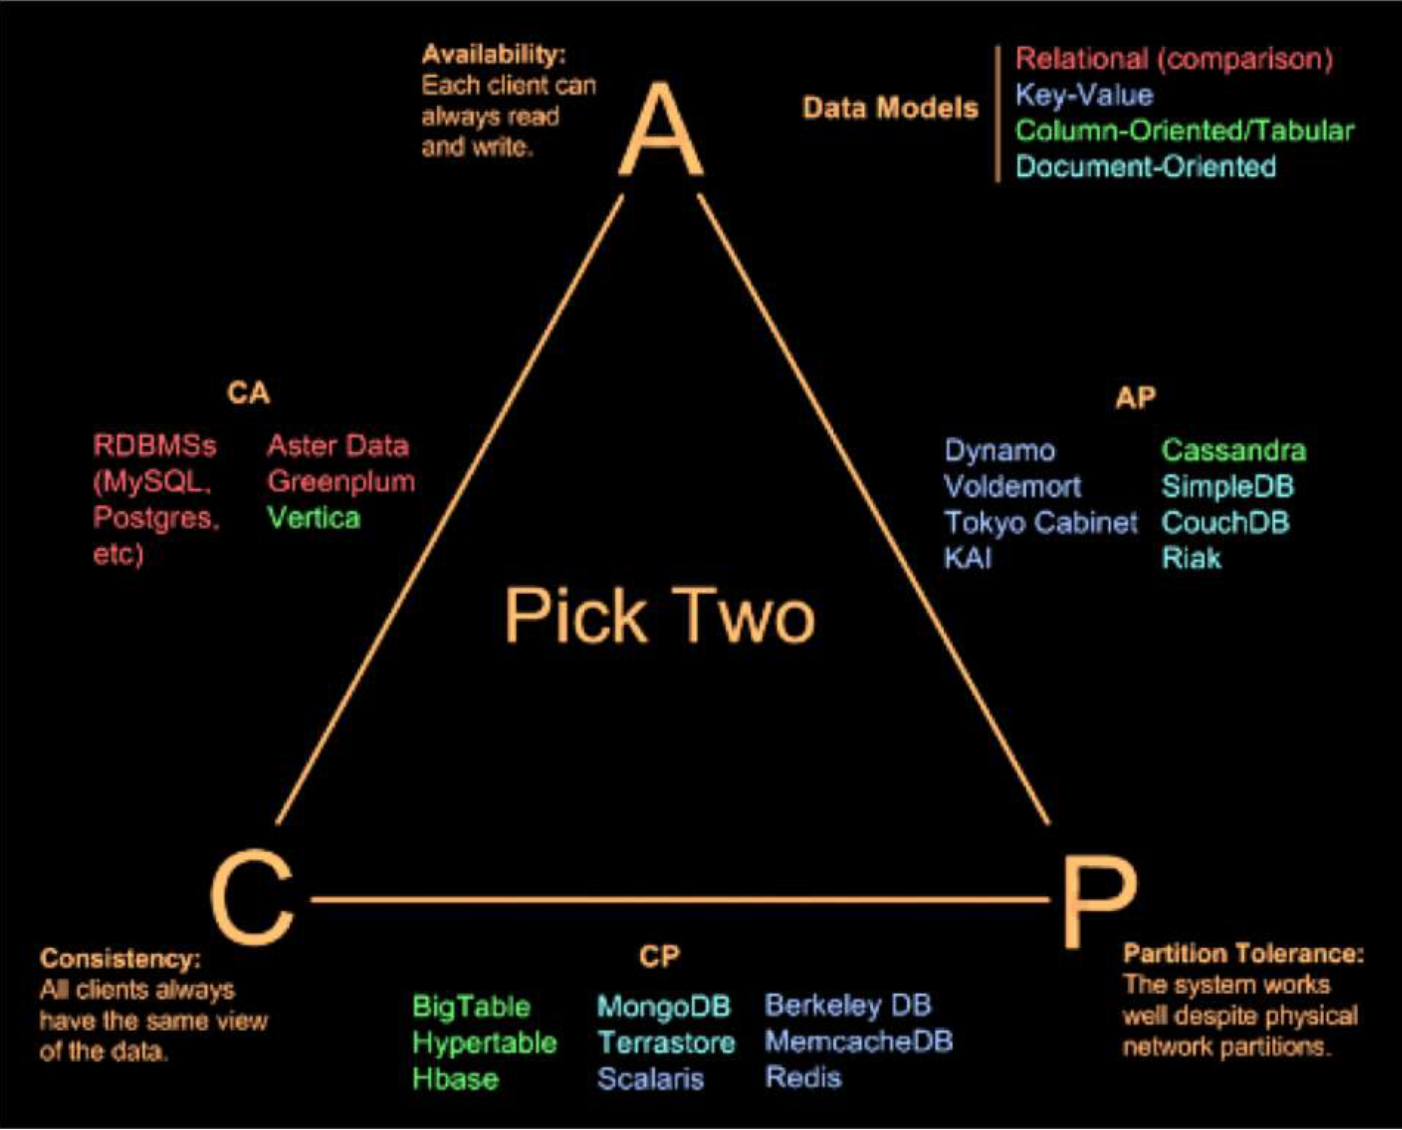
\includegraphics[width=300pt]{images/cap-theorem.png}\hspace*{\fill}
  \label{fig:cap-theorem}
  \caption{Visual Guide to CAP Theorem}
\end{figure} \\ \pagebreak
\subsubsection{ACID vs. BASE properties}
\textbf{SQL databases:}
\begin{itemize}
	\item Structured query language
	\item Traditional relational databases (unique keys, single valued, no update/insertion/deletion anomalies)
	\item Well structured data
	\item ACID properties should hold
\end{itemize}
\textbf{NoSQL (Not Only SQL) databases:}
\begin{itemize}
	\item Triggered by the storage needs of Web 2.0 companies such as Facebook, Google and Amazon.com
	\item Not necessarily well structured - e.g., pictures, documents, web page description, video clips, etc.
	\item \uline{ACID properties may not hold}, but this does not mean that there are no properties at all (there are new properties)
	\item focuses on availability of data even in the presence of multiple failures
	\item spread data across many storage systems with a high degree of replication
\end{itemize}
\textbf{BASE} properties are much weaker properties w.r.t. to ACID ones. The rationale behind them is that it's ok to use stale data and it's okay to give approximate answers. 
\begin{itemize}
	\item \uline{\textbf{B}asic \textbf{A}vailability}: fulfill request, even in partial consistency. Basic functionalities are always provided.
	\item \uline{\textbf{S}oft State}: abandon the consistency requirements of the ACID model pretty much completely.
	\item \uline{\textbf{E}ventual consistency}: at some point in the future, data will converge to a consistent state; delayed consistency, as opposed to immediate consistency of the ACID properties.
	\begin{itemize}
		\item purely a liveness guarantee (reads eventually return the requested value);
		\item no safety guarantees, i.e., an eventually consistent system can return any value before it converges
	\end{itemize}
\end{itemize}
\subsubsection{The NoSQL World}
\center{\textit{Google, Amazon, Facebook, and DARPA all recognized that \textbf{when you scale systems large enough, you can never put enough iron in one place to get the job done} (and you wouldn’t want to, to prevent a single point of failure).
Once you accept that you \textbf{have a distributed system, you need to give up consistency or availability}, which the fundamental transactionality of traditional RDBMSs cannot abide.} - Cedric Beust}
\\ \raggedright \vspace{0.5em}
The acronym \textbf{NoSQL} was first used in 1998 by Carlo Strozzi while naming his lightweight, open-source "relational" database that did not use SQL. NoSQL term was used to say that he was not using an SQL interface. \\ 
The term was then reintroduced in early 2009, when Eric Evans and Johan Oskarsson used it to describe non-relational databases (which are often referred to as SQL systems). In that case the term was meaning "not only SQL" to emphasize the fact that some systems might even support SQL-like query languages.
\paragraph{\uline{Kind of NoSQL}}
NoSQL solutions fall into two major areas:
\begin{itemize}
	\item \textbf{Key/Value} or "the big hash table"
	\begin{itemize}
		\item Amazon S3 (Dynamo)
		\item Voldemort
		\item Scalaris
		\item Memcache DB
		\item Azure Table Storage
		\item Redis
		\item Riak
	\end{itemize}
	\item \textbf{Schema-less}
	\begin{itemize}
		\item Cassandra (column-based)
		\item CouchDB (document-based)
		\item Neo4J
		\item HBase
	\end{itemize}
\end{itemize}
\paragraph{\uline{Different types of NoSQL}}
\begin{itemize}
	\item \textbf{Key-Value Store}: A key that refers to a payload (actual content /data). \\ \textit{MemcacheDB, Azure Table Storage, Redis}
	\item \textbf{Column Store}: column data is saved together, as opposed to row data. Super useful for data analytics. \\ \textit{Hadoop, Cassandra, Hypertable}
	\item \textbf{Document / XML / Object Store}: key (and possibly other indexes) point at serialized object. DB can operate against values in document. \\ \textit{MongoDB, CouchDB, RavenDB}
	\item \textbf{Graph Store}: nodes are stored independently, and the relationship between nodes (edges) are stored with data. \\ \textit{Neo4J}
\end{itemize}
\begin{figure}[h!]
 \hfill 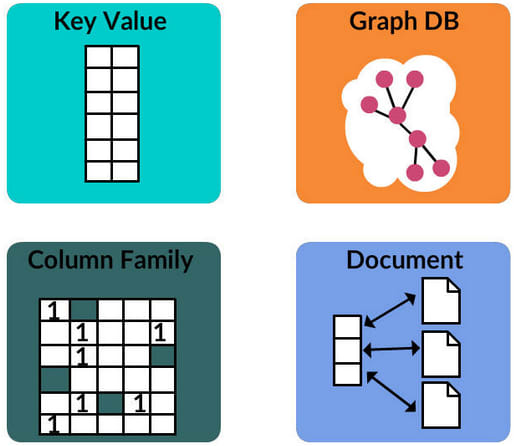
\includegraphics[width=150pt]{images/nosqltypes.jpeg}\hspace*{\fill}
  \label{fig:nosqltypes}
  \caption{NoSQL types}
\end{figure} 
\pagebreak
Most of NoSQL databases are open source projects started and/or supported by the most famous companies in the world, cause they needed to create custom solutions to improve their performance.
\begin{itemize}
	\item Google $\rightarrow$ BigTable, LevelDB
	\item LinkedIn $\rightarrow$ Voldemort
	\item Facebook $\rightarrow$ Cassandra
	\item Twitter $\rightarrow$ Hadoop/HBase, FlockDB, Cassandra
	\item Netflix $\rightarrow$ SimpleDB, Hadoop/HBase, Cassandra
	\item CERN $\rightarrow$ CouchDB
\end{itemize}
This is a big shift from traditional SQL-based produced by companies such as Oracle, IBM and Microsoft. They are still selling traditional, relational and transactional DBMS. Indeed, their projects are not open source. \\ \vspace{1em}
In conclusion, there is no general answer to whether your application needs an ACID versus BASE consistency model. Given BASE's loose consistency, developers need to be more \textbf{knowledgeable and rigorous about consistent data} if they choose a BASE store for their application. Planning around BASE limitations can sometimes be a major disadvantage when compared to the simplicity of ACID transactions. A fully ACID database is the perfect fit for use cases where data reliability and consistency are essential.
\begin{figure}[h!]
 \hfill 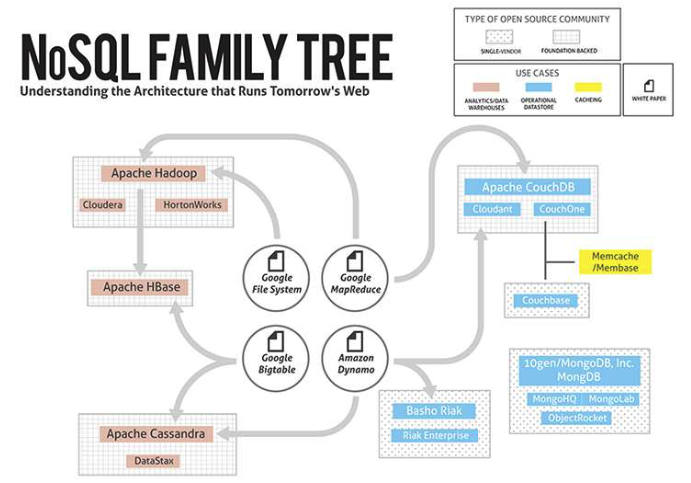
\includegraphics[width=350pt]{images/nosqlfamtree.png}\hspace*{\fill}
  \label{fig:nosqlfamtree}
\end{figure} 
\section{Graph DB}
Graph databases address one of the great macroscopic business trends of today: leveraging complex and dynamic relationships in highly connected data to generate insight and competitive advantage. For data of any significant size or value, graph databases are the best way to represent and query connected data. Connected data is data whose interpretation and value requires us first to understand the ways in which its constituent elements are related. \nline
Although large corporations realized this some time ago and began creating their own proprietary graph processing technologies, we are now in an era where that technology has rapidly become democratized. Today, general-purpose graph databases are a reality, enabling mainstream users to experience the benefits of connected data without having to invest in building their own graph infrastructure.
\nline
Graph theory was pioneered by Euler in the 18th century, and has been actively researched and improved by mathematicians, sociologists, anthropologists, and other practitioners ever since. However, it is only in the past few years that graph theory and graph thinking have been applied to information management. In that time, graph databases have helped solve important problems in the areas of social networking, master data management, geospatial, recommendations, and more. This increased focus on graph databases is driven by two forces: by the massive commercial success of companies such as Facebook, Google, and Twitter, all of whom have centered their business models around their own proprietary graph technologies; and by the introduction of general-purpose graph databases into the technology landscape.
\subsection{Graph Theory}
Formally, a graph is just a collection of \textit{vertices} and \textit{nodes} $-$ or, in other words, a set of \textit{nodes} and the \textit{relationships} that connect them. Graphs represent entities as nodes and the ways in which those entities relate to the world as relationships. This general-purpose expressive structure allows us to model all kinds of scenarios that we can imagine.
Indeed, graphs are extremely useful in understanding a wide diversity of datasets in fields such as science, government, and business. \\ For example, Twitter's data is represented as a graph. In Figure 25 we ee a small network of Twitter users. Each node is labeled \textit{User}, indicating its role in the network. These nodes are then connected with relationships, which help further establish the semantic context: namely, that Billy follows Harry, and that Harry, in turn, follows Billy. Ruth and Harry likewise follow each other, but sadly, although Ruth follows Billy, Billy hasn't (yet) reciprocated.
\begin{figure}[h!]
 \hfill 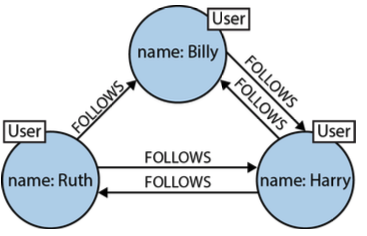
\includegraphics[width=180pt]{images/twitter-graph.png}\hspace*{\fill}
  \caption{A small social graph}
\end{figure} \\
Of course, Twitter’s real graph is hundreds of millions of times larger than the example in Figure 25, but it works on precisely the same principles. In Figure 26 we’ve expanded the graph to include the messages published by Ruth. \pagebreak
\begin{figure}[h!]
 \hfill 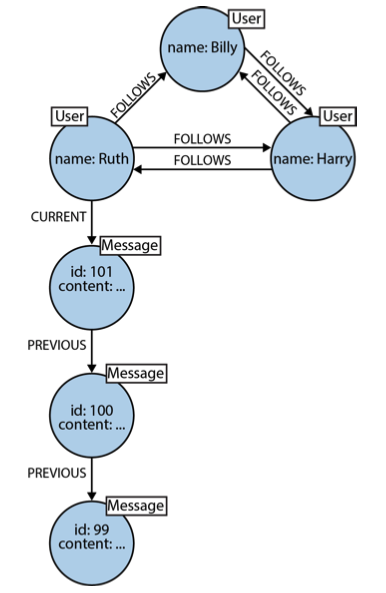
\includegraphics[width=150pt]{images/twitter-graph2.png}\hspace*{\fill}
  \caption{Publishing messages}
\end{figure} \\
Though simple, Figure 26 shows the expressive power of the graph model. It’s easy to see that Ruth has published a string of messages. Her most recent message can be found by following a relationship marked CURRENT. The PREVIOUS relationships then create Ruth’s timeline. \nline
In discussing Figure 26 we’ve also informally introduced the most popular form of graph model, the \textbf{labeled property graph}. A labeled property graph has the following characteristics:
\begin{itemize}
	\item It contains nodes and relationships
	\item Nodes contain properties (key-value pairs)
	\item Nodes can be labeled with one or more labels
	\item Relationships are named and directed, and always have a start and end node
	\item Relationships can also contain properties
\end{itemize}
\subsubsection{Useful definitions}
\textbf{Vertex}
\begin{itemize}
	\item Basic element
	\item Drawn as a node or a dot
	\item Vertex set of G is usually denoted by $V(G)$, or $V$
\end{itemize}
\textbf{Edge}
\begin{itemize}
	\item A set of two elements
	\item Drawn as a line connecting two vertices, called end vertices, or endpoints
	\item The edge set of G is usually denoted by $E(G)$, or $E$
\end{itemize} \pagebreak
\begin{figure}[h!]
 \hfill 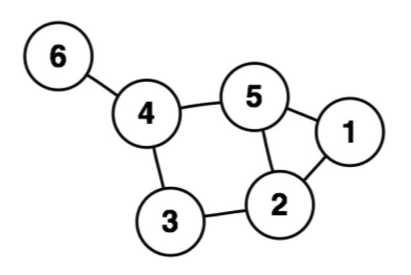
\includegraphics[width=150pt]{images/graph-example.png}\hspace*{\fill}
  \caption{$V:= \{1,2,3,4,5,6\} - E: \{ \{1,2\},\{1,5\},\{2,3\},\{2,5\},\{3,4\},\{4,5\},\{4,6\}\}$}
\end{figure}
\textbf{Simple graphs}: simple graphs are graphs without multiple edges or self-loops.
\nline
\textbf{Path}: a path is a sequence of vertices such that there is an edge from each vertex to its successor. A path is \uline{simple} if each vertex is distinct.
\begin{figure}[h!]
 \hfill 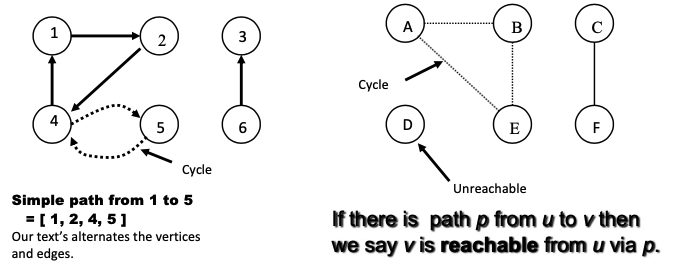
\includegraphics[width=250pt]{images/graph-path.png}\hspace*{\fill}
  \caption{Graph path and reachability}
\end{figure} \\
\textbf{Cycle}: a path from a vertex to itself is called cycle. A graph is called \uline{cyclic} if it contains a cycle; otherwise it is called \uline{acyclic}
\begin{figure}[h!]
 \hfill 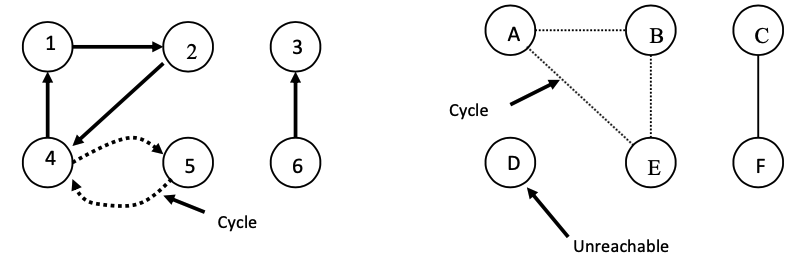
\includegraphics[width=220pt]{images/graph-cycle.png}\hspace*{\fill}
  \caption{Graph cycle}
\end{figure} \\
\textbf{Connectivity}: a graph is \uline{connected} if and only if
\begin{itemize}
	\item you can get from any node to any other by following a sequence of edges OR
	\item any two nodes are connected by a path
\end{itemize}
A directed graph is \uline{strongly connected} if there is a directed path from any node to any other node. \nline
\textbf{Sparse/Dense}
\begin{itemize}
	\item A graph is \uline{sparse} if $|E| \approx |V|$ (same number of edges and vertices $\rightarrow$ very few connections)
	\item A graph is \uline{dense} if $|E| \approx |V|^2$ (graph full of connections $\rightarrow$ with $n$ vertices, there can be a max of $n(n-1)$ edges)
\end{itemize}
 \pagebreak
\textbf{Weighted Graph}: is a graph for which each edge has an associated \uline{weight}, usually given by a weight function $w:E\rightarrow R$.
\begin{figure}[h!]
 \hfill 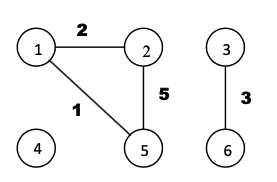
\includegraphics[width=150pt]{images/graph-weight.png}\hspace*{\fill}
  \caption{For example, in a GPS navigator we could use weight to specify duration, distance or traffic. The shortest path between two nodes is then calculated selecting the edges with the lowest weight.}
\end{figure}  \\
\textbf{Directed Graph}: edges have directions and the arch can be followed only in that direction
\nline
\textbf{Bipartite Graph}: V can be partitioned into 2 sets $V_1$ and $V_2$ such that $(u,v) \in E$ implies:
\begin{itemize}
	\item either $u \in V_1$ and $v \in V_2$
	\item OR $v \in V_1$ and $u \in V_2$
\end{itemize}
\begin{figure}[h!]
 \hfill 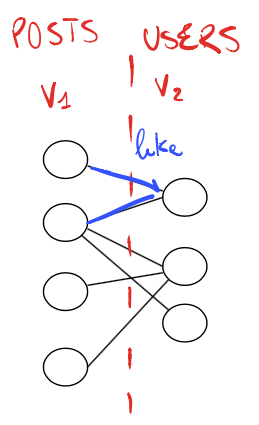
\includegraphics[width=120pt]{images/bipartite-graph.png}\hspace*{\fill}
  \caption{Nodes in $V_1$ connects only with nodes in $V_2$ (usually those are different categories of nodes e.g., Users and Posts)}
\end{figure} 
\textbf{Complete Graph}: denoted by $K_n$, in a complete graph every pair of vertices are adjacent with a total of $n(n-1)$ edges.
\begin{figure}[h!]
 \hfill 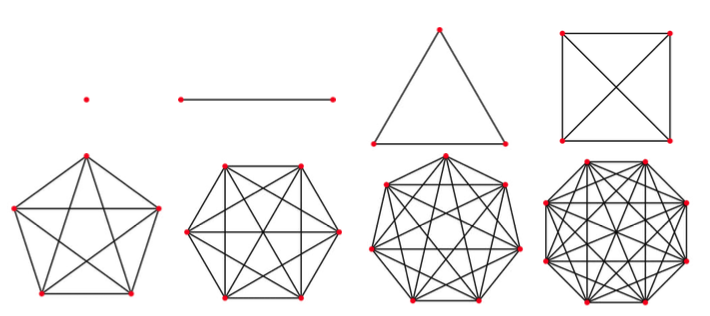
\includegraphics[width=160pt]{images/complete-graph.png}\hspace*{\fill}
  \caption{Exponential growth}
\end{figure}  \\
\pagebreak
\textbf{Planar Graph}: can be drawn on a plane such that no two edges intersect. \nline
\textbf{Tree}: is a \uline{connected acyclic graph} where two nodes have exactly one path between them.
\begin{figure}[h!]
 \hfill 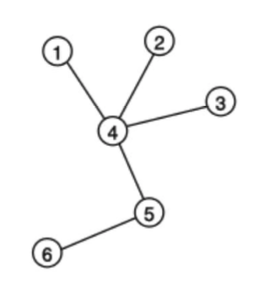
\includegraphics[width=100pt]{images/tree-graph.png}\hspace*{\fill}
  \caption{Example of Tree}
\end{figure}  \\
\textbf{Degree}: number of edges incident on a node \\
\textbf{Degree (directed graph)}: 
\begin{itemize}
	\item \uline{In degree}: number of edges entering the node
	\item \uline{Out degree}: number of edges leaving the node
	\item $Degree = indegree + outdegree$
\end{itemize}
\begin{figure}[h!]
\begin{minipage}{.5\textwidth}
  \centering
  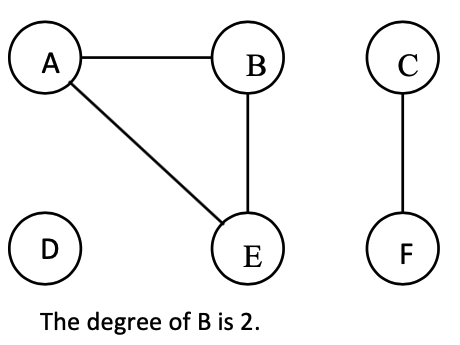
\includegraphics[width=.5\linewidth]{images/graph-degree}
  \captionof{figure}{Node degree}
\end{minipage}%
\begin{minipage}{.5\textwidth}
  \centering
  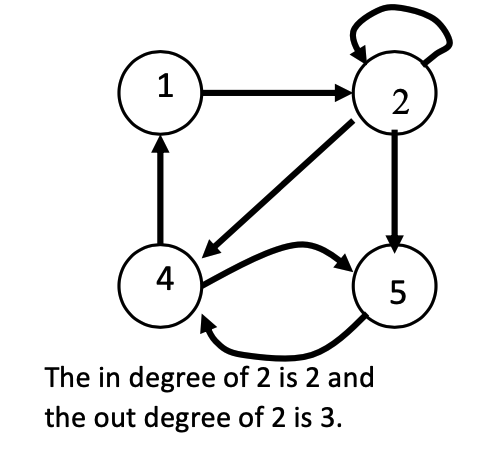
\includegraphics[width=.5\linewidth]{images/directed-graph-degree}
  \captionof{figure}{Node degree in directed graph}
\end{minipage}
\end{figure}
\textbf{Subgraph}: vertex and edge sets are subsets of those of G; a \uline{supergraph} of a graph G is a graph that contains G as a subgraph.
\begin{figure}[h!]
 \hfill 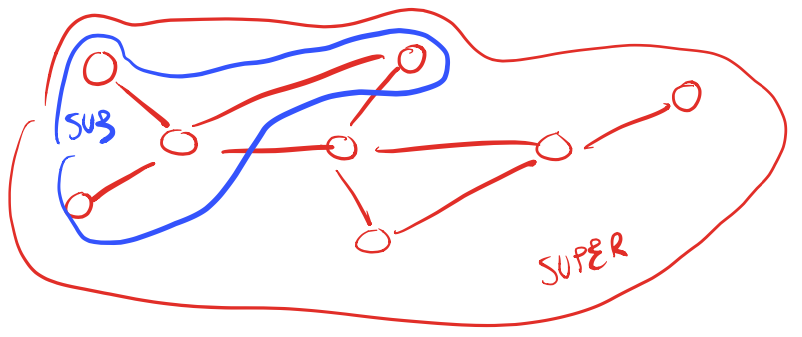
\includegraphics[width=150pt]{images/subgraph.png}\hspace*{\fill}
  \caption{Subgraph and Supergraph}
\end{figure} 
\pagebreak
\subsubsection{Graph Abstract Data Type (ADT)}
In computer science, a graph is an abstract data type (ADT) that consists of:
\begin{itemize}
	\item a set of nodes
	\item a set of edges (establish relationships/connections between the nodes)
\end{itemize}
The graph ADT follows directly from the graph concept from mathematics. We can implement a graph as a:
\begin{itemize}
	\item Matrix
	\begin{itemize}
		\item Incidence Matrix - [edge, vertex] contains the edge's data
		\item Adjacency Matrix - [vertex, vertex] boolean values (adjacent or not) or edge weights
	\end{itemize}
	\item List
	\begin{itemize}
		\item Edge List - pairs (ordered if directed) of vertices and optionally weight and other data
		\item Adjacency List
	\end{itemize}
\end{itemize}
\begin{figure}[h!]
 \hfill 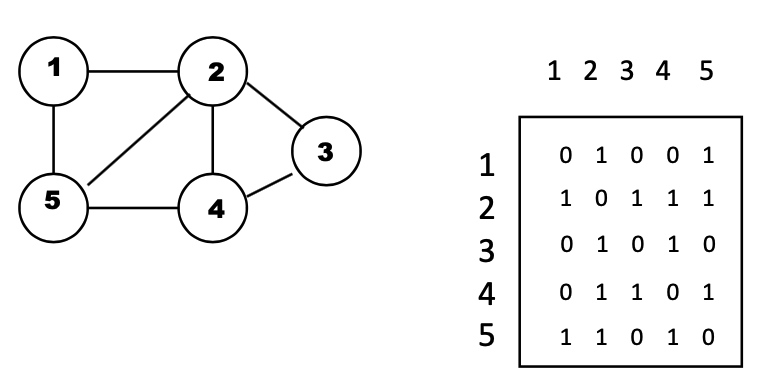
\includegraphics[width=100pt]{images/adjacency-matrix.png}\hspace*{\fill}
  \caption{$|V|x|V|$ matrix $A=(a_{ij})$ such that $a_{ij}=1$ if $(i,j) \in E$ and $0$ otherwise.}
\end{figure} 
\subsection{Graph Databases}
A \textbf{graph database management system} (henceforth, a graph database) is an online database management system with Create, Read, Update, and Delete (CRUD) methods that expose a graph data model. Graph databases are generally built for use with transactional (OLTP) systems. Accordingly, they are normally optimized for transac‐ tional performance, and engineered with transactional integrity and operational availability in mind. \nline
There are two properties of graph databases we should consider when investigating graph database technologies:
\begin{itemize}
	\item \textit{The underlying storage}: \\ Some graph databases use \uline{native graph storage} that is optimized and designed for storing and managing graphs. Not all graph database technologies use native graph storage, however. Some serialize the graph data into a relational database, an object-oriented database, or some other general-purpose data store.
	\item \textit{The processing engine}: \\ Some definitions require that a graph database use index-free adjacency, meaning that \uline{connected nodes physically “point” to each other in the database}. Here we take a slightly broader view: any database that from the user’s perspective behaves like a graph database (i.e., exposes a graph data model through CRUD operations) qualifies as a graph database. We do acknowledge, however, the significant performance advantages of index-free adjacency, and therefore use the term native graph processing to describe graph databases that leverage index-free adjacency.
\end{itemize}
\textcolor{blue}{\textit{It’s important to note that native graph storage and native graph processing are neither good nor bad $-$ they’re simply classic engineering trade-offs. The benefit of native graph storage is that its purpose-built stack is engineered for performance and scalability. The benefit of nonnative graph storage, in contrast, is that it typically depends on a mature nongraph backend (such as MySQL) whose production characteristics are well understood by operations teams. Native graph processing (index-free adjacency) benefits traversal performance, but at the expense of making some queries that don’t use traversals difficult or memory intensive.}} 
\nline
Relationships are first-class citizens of the graph data model. This is not the case in other database management systems, where we have to infer connections between entities using things like foreign keys or out-of-band processing such as map-reduce. By assembling the simple abstractions of nodes and relationships into connected structures, graph databases enable us to build arbitrarily sophisticated models that map closely to our problem domain. The resulting models are simpler and at the same time more expressive than those produced using traditional relational databases and the other NoSQL (Not Only SQL) stores.
\subsubsection{Advantages of Graph Databases}
\paragraph{Performance:}
One compelling reason, then, for choosing a graph database is the sheer \uline{performance increase when dealing with connected data versus relational databases and NoSQL stores}. In contrast to relational databases, where join-intensive query performance deteriorates as the dataset gets bigger, with a graph database performance tends to remain relatively constant, even as the dataset grows. This is because queries are localized to a portion of the graph. As a result, the execution time for each query is proportional only to the size of the part of the graph traversed to satisfy that query, rather than the size of the overall graph.
\paragraph{Flexibility:}
As developers and data architects, we want to connect data as the domain dictates, thereby allowing structure and schema to emerge in tandem with our growing understanding of the problem space, rather than being imposed upfront, when we know least about the real shape and intricacies of the data. Graph databases address this want directly. 
\nline
Graphs are naturally additive, meaning we can add new kinds of relationships, new nodes, new labels, and new subgraphs to an existing structure without disturbing existing queries and application functionality. These things have generally positive implications for developer productivity and project risk. Because of the graph model’s flexibility, we don’t have to model our domain in exhaustive detail ahead of time $-$ a practice that is all but foolhardy in the face of changing business requirements. The additive nature of graphs also means we tend to perform fewer migrations, thereby reducing maintenance overhead and risk.
\paragraph{Agility:} 
We want to be able to evolve our data model in step with the rest of our application, using a technology aligned with today’s incremental and iterative software delivery practices. Modern graph databases equip us to perform frictionless development and graceful systems maintenance. In particular, the schema-free nature of the graph data model, coupled with the testable nature of a graph database’s application programming interface (API) and query language, empower us to evolve an application in a controlled manner. 
\nline
At the same time, precisely because they are schema free, graph databases lack the kind of schema-oriented data governance mechanisms we’re familiar with in the relational world. But this is not a risk; rather, it calls forth a far more visible and actionable kind of governance. Governance is typically applied in a programmatic fashion, using tests to drive out the data model and queries, as well as assert the business rules that depend upon the graph.
\begin{figure}[h!]
\begin{minipage}{.5\textwidth}
  \centering
  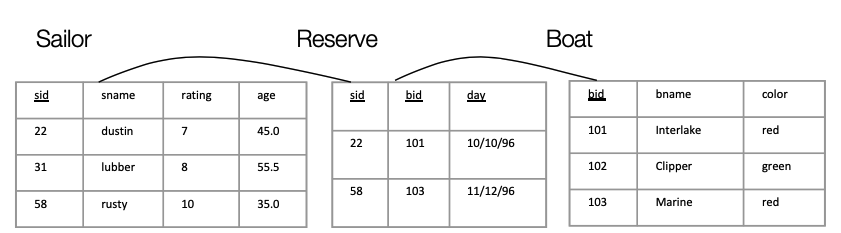
\includegraphics[width=.9\linewidth]{images/relational-db}
  \captionof{figure}{Relational DB with intermediate join table}
\end{minipage}%
\begin{minipage}{.5\textwidth}
  \centering
  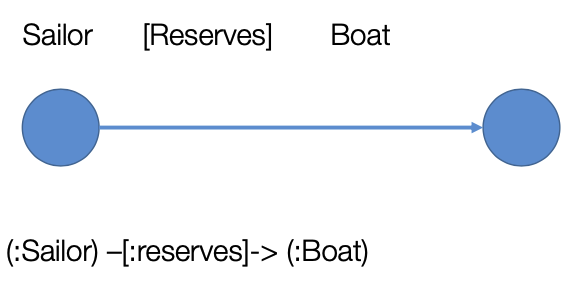
\includegraphics[width=.7\linewidth]{images/graph-db}
  \captionof{figure}{Graph DB model. Much simpler!}
\end{minipage}
\end{figure}
\begin{figure}[h!]
 \hfill 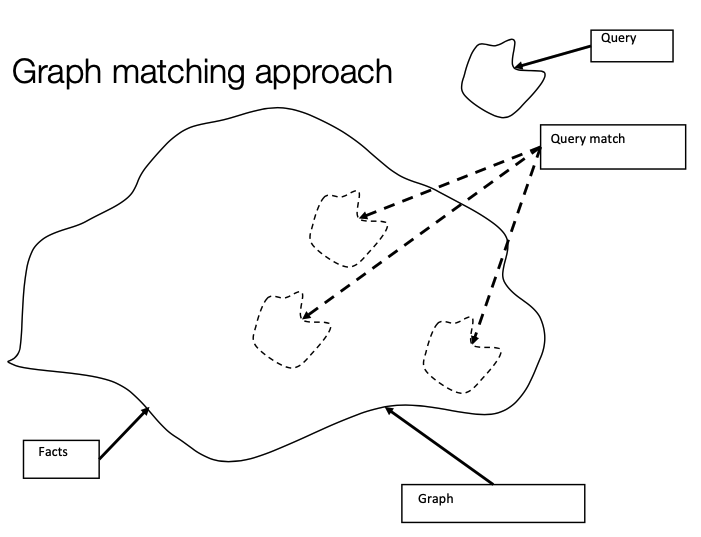
\includegraphics[width=150pt]{images/graph-query.png}\hspace*{\fill}
  \caption{Querying a graph is similar to pattern matching. First, we define a pattern (shape of (sub)graph that we are looking for) and then we look in the graph for that shape.}
\end{figure}  \\
\pagebreak
\subsection{Neo4J}
\textbf{Neo4J} is the most popular graph database, developed by Neo Technologies and implemented in Java. It is fully open source. \\
\uline{Salient features}
\begin{itemize}
	\item \textbf{Neo4J is schema free}: data does not have to adhere to any convention
	\item \textbf{ACID}: atomic, consistent, isolated and durable for logical units of work (fully transactional solution)
	\item Easy to get started and use
	\item Well documented and large developer community
	\item Support for wide variety of languages (Java, Python, Perl, Scala, Cypher, etc.)
\end{itemize}
\begin{figure}[h!]
 \hfill \includegraphics[width=180pt]{images/neo4j-arch.png}\hspace*{\fill}
  \caption{Neo4J software architecture. Each type of record (e.g., nodes, relationships) is stored in a separate and dedicated file. Traditional \textbf{C}onsistency and \textbf{Availability} support (no partitioning).}
\end{figure} 
Neo4J is meant to be an operational DB, not specifically for analytics. Thus, it is efficient on nodes and patterns, while is not so efficient in whole-graph analysis. \nline
The data model is composed by 
\begin{itemize}
	\item Nodes $-$ with labels (type) and attributes
	\item Edges
	\item Indexes (different from the ones in standard relational db) indexe
\end{itemize}
\subsubsection{Cypher}
Cypher is an expressive (yet compact) graph database query language. Cypher is arguably the easiest graph query language to learn, and is a great basis for learning about graphs. Cypher is designed to be easily read and understood by developers, database profes‐ sionals, and business stakeholders. Its ease of use derives from the fact that it is in accord with the way we intuitively describe graphs using diagrams. 
\nline
Cypher enables a user (or an application acting on behalf of a user) to ask the database to find data that matches a specific pattern. Colloquially, we ask the database to “find things like this.” And the way we describe what “things like this” look like is to draw them, using ASCII art.
\begin{figure}[h!]
 \hfill \includegraphics[width=150pt]{images/cypher-pattern.png}\hspace*{\fill}
  \caption{This pattern describes three mutual friends. Here’s the equivalent ASCII art representation in Cypher: \textcolor{blue}{(emil)$\leftarrow$[:KNOWS]$-$(jim)$-$[:KNOWS]$\rightarrow$(ian)$-$[:KNOWS]$\rightarrow$(emil)}
}
\end{figure}  \\
Cypher patterns follow very naturally from the way we draw graphs on the whiteboard.
\nline
The previous Cypher pattern describes a simple graph structure, but it doesn’t yet refer to any particular data in the database. To bind the pattern to specific nodes and relationships in an existing dataset we must specify some property values and node labels that help locate the relevant elements in the dataset. For example:

\begin{figure}[h!]
 \hfill \includegraphics[width=150pt]{images/cypher-pattern2.png}\hspace*{\fill}
  \caption{Here we have bound each node to its identifier using its $name$ property and $Person$ label. The $emil$ identifer, for example, is bound to a node in the dataset with a label $Person$ and a $name$ property whose value is $Emil$. Anchoring parts of the pattern to real data in this way is normal Cypher practice.}
\end{figure} 

Like most query languages, Cypher is composed of clauses. The simplest queries consist of a $MATCH$ clause followed by a $RETURN$ clause (we’ll describe the other clauses you can use in a Cypher query later in this chapter). Here’s an example of a Cypher query that uses these three clauses to find the mutual friends of a user named Jim:
\begin{figure}[h!]
 \hfill \includegraphics[width=250pt]{images/cypher-pattern3.png}\hspace*{\fill}
\end{figure}  \\
Other Cypher clauses:
\begin{itemize}
	\item \textbf{WHERE}: provides criteria for filtering pattern matching results.
	\item \textbf{CREATE} and \textbf{CREATE UNIQUE}: create nodes and relationships.
	\item \textbf{MERGE}: ensures that the supplied pattern exists in the graph, either by reusing existing nodes and relationships that match the supplied predicates, or by creating new nodes and relationships.
	\item \textbf{DELETE}: removes nodes, relationships, and properties.
	\item \textbf{SET}: sets property values.
	\item \textbf{FOREACH}: performs an updating action for each element in a list.
	\item \textbf{UNION}: merges results from two or more queries.
	\item \textbf{WITH}: chains subsequent query parts and forwards results from one to the next. Similar to piping commands in Unix.
	\item \textbf{START}: specifies one or more explicit starting points $-$ nodes or relationships $-$ in the graph. (START is deprecated in favor of specifying anchor points in a MATCH clause.)
\end{itemize}
\begin{figure}[h!]
 \hfill \includegraphics[width=150pt]{images/cypher-ex-query2.png}\hspace*{\fill}
 \caption{\textbf{Example query.} Find a node $n$ of type $Crew$ connected to $m$ with relations $r$ of type $Knows$ (from 1-step to *-steps in the relation) }
\end{figure}
\begin{figure}[h!]
 \hfill \includegraphics[width=150pt]{images/cypher-ex-query.png}\hspace*{\fill}
 \caption{\textbf{Example query.} Aggregation can be used (count). WITH separates query parts explicitly, to declare the variables for the next part. SKIP skips results at the top and LIMIT limits the number of results. }
\end{figure}
\begin{figure}[h!]
 \hfill \includegraphics[width=180pt]{images/cypher-ex-pattern1.png}\hspace*{\fill}
\end{figure}
\begin{figure}[h!]
 \hfill \includegraphics[width=250pt]{images/cypher-ex-pattern2.png}\hspace*{\fill}
   \caption{List of patterns}
\end{figure}
\paragraph{Stored procedures}
Cypher support stored procedures. It allows you to add JAVA functions or simply move a JAR to a folder to add new functions. Of course, there are also some predefined function such as \textit{shortestPath, allShortestPaths, size}.
\paragraph{Hints}
\begin{itemize}
	\item \textbf{Use parameters instead of literals} when possible. This allows Cypher to re-use your queries instead of having to parse and build new execution plans.
	\item \textbf{Always set an upper limit for your variable length patterns.} It’s easy to have a query touch all nodes in a graph by mistake.
	\item \textbf{Return only the data you need.} Avoid returning whole nodes and relationships
	\item Use \textbf{PROFILE / EXPLAIN} to analyze the performance of your queries.
\end{itemize}
\pagebreak
\section{Key-Value DB}
The main motivation behind Key-Value databases is performance. Indeed, there are certain organizations/companies that cannot accept low performances:
\begin{itemize}
	\item Amazon - Every 1/10 second delay resulted in 1\% loss of sales.
	\item Google - Half a second delay caused a 20\% drop in traffic
	\item Industrial Group - 1-second delay in page-load time
	\begin{itemize}
		\item 11\% fewer page views
		\item 15\% decrease in customer satisfaction
		\item 7\% loss in conversions
	\end{itemize}
\end{itemize}
Search by ID is usually built on top of a key-value store.
\begin{itemize}
	\item \uline{(Business) Key $\rightarrow$ Value} (follow this schema)
	\item (twitter.com) tweet $\rightarrow$ information about tweet
	\item (kayak.com) flight number $\rightarrow$ information about flight
	\item (yourbank.com) account number $\rightarrow$ information about it
	\item (amazon.com) item number $\rightarrow$ information about it
\end{itemize}
\subsection{How does a key-value database work?}
A key-value database, aka key-value store, associates a value (which can be anything from a number or simple string, to a complex object) with a key, which is used to keep track of the object. In its simplest form, a key-value store is like a dictionary/array/map object as it exists in most programming paradigms, but which is stored in a persistent way and managed by a Database Management System (DBMS). \nline
Key-value databases use compact, efficient index structures to be able to quickly and reliably locate a value by its key, making them ideal for systems that need to be able to find and retrieve data in constant time. Redis, for instance, is a key-value database that is optimized for tracking relatively simple data structures (primitive types, lists, heaps, and maps) in a persistent database. By only supporting a limited number of value types, Redis is able to expose an extremely simple interface to querying and manipulating them, and when configured optimally is capable of extremely high throughput. \nline
\subsubsection{Key Features}
A key-value database is defined by the fact that it allows programs or users of programs to retrieve data by keys, which are essentially names, or identifiers, that point to some stored value. Because key-value databases are defined so simply, but can be extended and optimized in numerous ways, there is no global list of features, but there are a few common ones:
\begin{itemize}
	\item \textbf{Retrieving a value} (if there is one) stored and associated with a given key
	\item \textbf{Deleting the value} (if there is one) stored and associated with a given key
	\item \textbf{Setting, updating, and replacing the value} (if there is one) associated with a given key
\end{itemize}

\subsection{Redis}
\textbf{RE}mote \textbf{DI}ctionary \textbf{S}erver (REDIS) introduced their key-value database in 2009. \nline
Redis is an advanced key-value store, where keys can contain data structures such as strings, hashes, lists, sets, and sorted sets. Supporting a set of atomic operations on these data types. \\
Redis is a different evolution path in the key-value databases where values are complex data types that are closely related to fundamental data structures and are exposed to the programmer as such, without additional abstraction layers. \\
It can be used as:
\begin{itemize}
	\item \textbf{Database} - Redis can persist data to disk
	\item \textbf{Caching layer} - Redis is fast
	\item \textbf{Message Broker} - Redis is not only a key-value store
\end{itemize}
What is \uline{NOT} Redis:
\begin{itemize}
	\item \textbf{Redis is not a replacement for Relational Databases} nor Document Stores.
	\item \textbf{It might be used complementary to a SQL relational store}, and/or NoSQL document store.
	\item Even when Redis offers configurable mechanisms for persistency, increased persistency will tend to increase latency and decrease throughput.
	\item \textbf{Best used for rapidly changing data} with a foreseeable database size (should fit mostly in memory).
\end{itemize}
Redis use cases:
\begin{itemize}
	\item Caching
	\item Counting things
	\item Blocking queues
	\item Pub/Sub (service bus)
	\item MVC Output Cache provider
	\item ASP.NET Session State provider
	\item Online user data (e.g., shopping cart, ...)
	\item ... any real-mine cross-platform, cross-application communication
\end{itemize}
\uline{When to consider Redis:}
\begin{itemize}
	\item \textbf{Speed is critical}
	\item More than just key-value pairs
	\item Dataset can fit in memory
	\item Dataset is not critical
\end{itemize}


\begin{figure}[ht!]
	\centering
	 \hfill \includegraphics[width=350pt]{images/redis-datatypes.png}\hspace*{\fill}
 \caption{Redis data types.}
 
 	\vspace{2em}
  \centering
  \hfill \includegraphics[width=250pt]{images/redis-commands1.png}\hspace*{\fill}

  \vspace{0.5em}

  \hfill \includegraphics[width=250pt]{images/redis-commands2.png}\hspace*{\fill}
 \caption{Redis commands. \href{https://redis.io/commands}{Full command reference here}}
\end{figure} 
\clearpage
\subsubsection{Scaling Redis}
\begin{itemize}
	\item \textbf{Persistence}: how can we be sure that we have some persistent storage of data (since Redis works in main memory)? \\ For this reason, REDIS provides two mechanisms to deal with persistence (very basic options):
	\begin{itemize}
		\item \uline{Redis Database Snapshots (RDB)}: save memory snapshot on disk (like a backup)
		\item \uline{append-only files (AOF)}: store in append mode the evolution of data
	\end{itemize}
	\item \textbf{Replication}: a Redis instance known as the \textit{master}, ensures that one or more instances known as the \textit{slaves}, become exact copies of the master. Clients can connect to the master or to the slaves. Slaves are read only by default, while master allows both read and write operations.
	\item \textbf{Partitioning}: we need to deal with data separation, breaking up data and distributing it across different hosts in a cluster. It can be implemented in different layers:
	\begin{itemize}
		\item \uline{Client}: partitioning on client-side code
		\item \uline{Proxy}: an extra layer that proxies all redis queries and performs partitioning \\ (i.e. \textcolor{blue}{Twemproxy})
		\item \uline{Query Router}: instances will make sure to forward the query to the right node\\  (i.e. \textcolor{blue}{Redis Cluster})
	\end{itemize}
	\item \textbf{Failover}: replace possible masters that are broken with a slave
	\begin{itemize}
		\item Manual
		\item Automatic with Redis Sentinel (for master-slave topology)
		\item Automatic with Redis Cluster (for cluster topology)
	\end{itemize}
\end{itemize}

\subsubsection{Redis topologies}

\begin{enumerate}
	\item Standalone
	\item Sentinel (automatic failover)
	\item Twemproxy (distribute data)
	\item Cluster (automatic failover and distribute data)
\end{enumerate}

\paragraph{I - Standalone} 
\begin{itemize}
	\item The master data is optionally replicated to slaves.
	\item The slaves provides data redundancy, reads offloading and save-to-disk offloading.
	\item Clients can connect to the Master for read/write operations or to the Slaves for read operations.
	\item Slaves can also replicate to its own slaves.
	\item There is no automatic failover.
\end{itemize}

\begin{figure}[h!]
 \hfill \includegraphics[width=270pt]{images/redis-standalone.png}\hspace*{\fill}
\end{figure} 

\paragraph{II - Sentinel} 
\begin{itemize}
	\item Redis Sentinel provides a reliable \textbf{automatic failover} in a master/slave topology, automatically promoting a slave to master if the existing master fails.
	\item Every deployment (master or slave) have a sentinel component that is able to check the status of the other servers. If the master goes down, a slave is selected to become a new master automatically.
	\item Sentinel does not distribute data across nodes.
\end{itemize}

\begin{figure}[h!]
 \hfill \includegraphics[width=180pt]{images/redis-sentinel.png}\hspace*{\fill}
\end{figure} 

\paragraph{III - Twemproxy} 
\begin{itemize}
	\item \href{https://github.com/twitter/twemproxy}{Twemproxy} (a project by twitter) works  as a proxy between the clients and many Redis instances.
	\item Is able to \textbf{automatically distribute data} among different standalone Redis instances.
	\item Supports consistent hashing with different strategies and hashing functions
	\item Multi-key commands and transactions are not supported.
\end{itemize}

\begin{figure}[h!]
 \hfill \includegraphics[width=350pt]{images/redis-twemproxy.png}\hspace*{\fill}
\end{figure} 

\paragraph{IV - Cluster} 
\begin{itemize}
	\item Redis Cluster \textbf{distributed data} across different Redis instances and \textbf{perform automatic failover} if any problem happens to any master instance.
	\item All nodes are directly connected with a service channel.
	\item The keyspace is divided into hash slots. Different nodes will hold a subset of hash slot.
	\item Multi-key commands are only allowed for keys in the same  hash slot.
\end{itemize}

\begin{figure}[h!]
 \hfill \includegraphics[width=180pt]{images/redis-cluster.png}\hspace*{\fill}
\end{figure} 

\subsubsection{Redis Advantages}
\begin{itemize}
	\item Performance
	\item Availability
	\item Fault-Tolerance
	\item Scalability (adaptability)
	\item Portability
\end{itemize}

\begin{figure}[h!]
 \hfill \includegraphics[width=300pt]{images/redis-performance.png}\hspace*{\fill}
 \caption{\href{https://redislabs.com/blog/the-proven-redis-performance/}{NoSQL \& SQL response performance comparison}. \\ Num of operations per unit of time - Average query time}
\end{figure} 

\subsection{Key-Value and Caching}
\subsubsection{What is Caching?}
From Wikipedia: \\ \textit{"A cache is a collection of data duplicating original values stored elsewhere or computed earlier, where the original data is expensive to fetch (owing to longer access time) or to compute, compared to the cost of reading the cache."} 
\nline

\textbf{Anatomy}:
\begin{itemize}
	\item Simple key/value storage
	\item Simple operations
	\begin{itemize}
		\item save
		\item get
		\item delete
	\end{itemize}
\end{itemize}
\pagebreak
\textbf{Terminology}:
\begin{itemize}
	\item Storage cost
	\item Retrieval cost (network load / algorithm load)
	\item Invalidation (keeping data up to data / removing irrelevant data)
	\item Replacement policy:
	\begin{itemize}
		\item FIFO - First in First Out
		\item LFU - Least Frequently Used (replace the cache entry used the least often in the recent past)
		\item LRU - Least Recently Used (replace the least recently used items first)
		\item MRU - Most Recently Used (replace, in contrast to LRU, the most recently used items first)
		\item Random vs. Belady's algorithm (predicting the information that will not be needed for the longest time in the future and replace it)
	\end{itemize}	 
	\item Cache concepts:
	\begin{itemize}
		\item Cold Cache: when the cache is empty or has irrelevant data, so that CPU needs to do a slower read from main memory for your program data requirement. 
		\item Warm Cache: when the cache contains relevant data, and all the reads for your program are satisfied from the cache itself.
	\end{itemize}
	\item Cache Hit and Cache Miss
	\begin{itemize}
		\item Hit: when an application needs data and finds that data in the cache (avoiding to look for it in main memory)
		\item Miss:  when an application needs data and doesn’t find it in the cache, so then it has to go and find the data on disc (takes more time).
	\end{itemize}
	\item Typical stats:
	\begin{itemize}
		\item $hit\_ratio = hits / (hits + misses)$
		\item $miss\_ratio = 1-hit\_ratio$
	\end{itemize}
\end{itemize}
\textbf{When to cache?}
\begin{itemize}
	\item Caches are only efficient when the benefits of faster access outweights the overhead of checking and keeping your cache up to data
	\item More cache hits than cache misses
\end{itemize}
\textbf{Where are caches users?}
\begin{itemize}
	\item At hardware level (CPU, HDD)
	\item Operating systems (RAM)
	\item Web stack (browser cache, DNS cache, CDNs cache, application level)
	\item Applications
\end{itemize}
\pagebreak
\subsubsection{Memcached}
\begin{itemize}
	\item Free \& open-source, high-performance, distributed memory object caching system
	\item Generic in nature, intended for use in speeding up dynamic web applications by alleviating database load.
	\item Key/Value dictionary
	\item Now used by Netlog, Facebook, Flickr, Wikipedia, Twitter, Youtube ...
\end{itemize}
Technically, Memcached is a server, where client access over TCP or UDP. Servers can run in pools and are independent, clients manage the pool (e.g., 3 servers with 64GB mem each give you a single pool of 192GB storage for caching). \\
What to store in a memcache?
\begin{itemize}
	\item High demand (data used often)
	\item Expensive (data hard to compute)
	\item Common (data shared across users)
	\item typical examples:
	\begin{itemize}
		\item user sessions (often)
		\item user data (often, shared)
		\item homepage data (often, shared, expensive)
	\end{itemize}
\end{itemize}
\textbf{Memcached principles}
\begin{itemize}
	\item \textcolor{blue}{Very simple version of a data store}
	\item \textcolor{blue}{Lightweight technology with high-performance} (\textcolor{red}{comes at a cost})
 	\item \textcolor{blue}{Fast network access}: memcached servers close to other application servers
	\item \textcolor{red}{No persistency}: if your server goes down, data in memcached is gone
	\item \textcolor{red}{No redundancy / fail-over}
	\item \textcolor{red}{No replication}: single item in cache lives on one server only
	\item \textcolor{red}{No authentication}: not used in shared environments
	\item 1 key is maximum 1MB
	\item Keys are string of 250 characters
	\item No enumeration of keys: thus no list of valid keys in cache at certain moment)
	\item No active clean-up (only clean up when more space needed, LRU policy)
\end{itemize}
\begin{figure}[h!]
\centering
\begin{minipage}{.5\textwidth}
  \centering
  \includegraphics[width=.8\linewidth]{images/memcached-php}
  \captionof{figure}{Memcached PHP Client functions.}
\end{minipage}%
\begin{minipage}{.5\textwidth}
  \centering
  \includegraphics[width=.8\linewidth]{images/memcached-example}
  \captionof{figure}{Code for explicitly implementing caching.}
\end{minipage}
\end{figure}
\pagebreak
\section{Big Column DB}
\subsection{Introduction}
\subsubsection{Column wise vs. Row wise database}
A \textbf{columnar database stores data by columns} rather than by rows, which makes it suitable for analytical query processing, and thus for data warehouses. They're often used in data warehouses, the structured data repositories that businesses use to support corporate decision-making. \\
The major difference in both the datastores (row- vs column-based lies in the way they physically store the data on the disk. We know that persistent storage disks (hard disks) are organized in blocks and have following usual properties for reading/write operations. Head Seek operation is expensive in disks due to mechanical movement required. Read/Write is quite fast.
\begin{enumerate}
	\item The whole block with data is loaded into the memory for reading by the operating system. Any further read for data for this block will happen from memory and will be super fast.
	\item Read/Writing operations on disks are not slow. Only the seek operation is slow. i.e. to move the head to the correct block to perform the operation.
	\item Due to the above point — sequential read/writes are much faster on disks rather than the random access.
\end{enumerate}
Here comes the main difference between row and columnar DBs. \\
\textbf{Row oriented database tries to store whole row of the database in the same block but columnar database stores the values of the columns of subsequent in the same block} 
\nline
Indeed, columnar storage for database tables is an important factor in optimizing analytic query performance because it drastically reduces the overall disk I\/O requirements and reduces the amount of data you need to load from disk.
\nline
The following series of illustrations (from \href{https://docs.aws.amazon.com/redshift/latest/dg/c_columnar_storage_disk_mem_mgmnt.html}{Amazon Redshift documentation}) describe how columnar data storage implements efficiencies and how that translates into efficiencies when retrieving data into memory.
\begin{figure}[h!]
 \hfill \includegraphics[width=240pt]{images/columnar-vs-row1.png}\hspace*{\fill}
 \caption{Row-wise}
\end{figure}  \\
In a typical relational database table, each row contains field values for a single record. In row-wise database storage, data blocks store values sequentially for each consecutive column making up the entire row. In online transaction processing (OLTP) applications, most transactions involve frequently reading and writing all of the values for entire records, typically one record or a small number of records at a time. As a result, row-wise storage is optimal for OLTP databases.
\begin{figure}[h!]
 \hfill \includegraphics[width=240pt]{images/columnar-vs-row2.png}\hspace*{\fill}
 \caption{Column-wise}
\end{figure}  \\
Using columnar storage, each data block stores values of a single column for multiple rows. This means that reading the same number of column field values for the same number of records requires a third of the I/O operations compared to row-wise storage. In practice, using tables with very large numbers of columns and very large row counts, storage efficiency is even greater. An added advantage is that, since each block holds the same type of data, block data can use a compression scheme selected specifically for the column data type, further reducing disk space and I/O.
\nline
\subsubsection{Column storage}
\paragraph{Issues with today's workloads}
Column data storage were born to address the need of large scale data analysis.
\begin{itemize}
	\item Data large and unstructured
	\item Lots of random reads and writes
	\item Foreign keys rarely needed (we use more complex data structured)
	\item Actual needs:
	\begin{itemize}
		\item Incremental scalability
		\item Speed
		\item No single point of failure
		\item Low cost (TCO) and admin
		\item Scale out, not up
	\end{itemize}
\end{itemize}
Recalling the CAP Theorem, for which we can achieve at most 2 out of the 3 guarantees (Consistency, Availability and Partition-tolerance), usually column databases (e.g., Cassandra) focus on Availability and Partition-tolerance, supporting only Eventual (weak) Consistency. Indeed, they are mainly used in OLAP systems (online analytical processing) and data mining operations.
\begin{figure}[h!]
 \hfill \includegraphics[width=250pt]{images/column-vs-row.png}\hspace*{\fill}
 \caption{Column vs. Row data storage}
\end{figure} \\
\textcolor{blue}{\textbf{Pros}}:
\begin{itemize}
	\item Data compression (1000 TB compression come handy)
	\item Improved Bandwidth Utilization
	\item Improved Code Pipelining
	\item Improved Cache Locality
\end{itemize}
\textcolor{red}{\textbf{Cons}}
\begin{itemize}
	\item Increased Disk Seek Time
	\item Increased cost of Inserts
	\item Increased tuple reconstruction costs
\end{itemize}
\begin{figure}[h!]
\centering
\begin{minipage}{.5\textwidth}
  \centering
  \includegraphics[width=.7\linewidth]{images/tuple-reconstruction1}
  \captionof{figure}{Row based always read the entire row (constant time). Column based instead are more efficient when few bytes have to be read. Then there is a breakeven point after which row based databases become more efficient to read data.}
\end{minipage}%
\begin{minipage}{.5\textwidth}
  \centering
  \includegraphics[width=.7\linewidth]{images/tuple-reconstruction2}
  \captionof{figure}{Tuple reconstruction.}
\end{minipage}
\end{figure}
\paragraph{Compression}
Compression: find a better encoding without losing information
\begin{itemize}
	\item Trades I/O for CPU
	\item Increased column-store opportunities:
	\begin{itemize}
		\item Higher data value locality (spatial and temporal) in column stores, saving space and performance
		\item Techniques such as \textit{run length encoding} is far more useful
		\item Can use extra space to store multiple copies of data in different sort orders
	\end{itemize}
\end{itemize}
Example:
\begin{figure}[h!]
 \hfill \includegraphics[width=300pt]{images/column-compression-ex.png}\hspace*{\fill}
 \caption{Column compression example using Run Length encoding}
\end{figure} 
\pagebreak
\subsection{Cassandra}
Cassandra is a columnar database which was originally designed at Facebook and then open-sourced (now within Apache foundation. Many big companies use Cassandra: IBM, eBay, twitter, Adobe, Netflix, Spotify ...
\\
Cassandra can be considered an hybrid of Google's Bigtable (columnar) and Amazon's Dynamo (key-value). By the way it emphasizes a lot on columnar features.
\begin{figure}[h!]
 \hfill \includegraphics[width=350pt]{images/cassandra-data-model.png}\hspace*{\fill}
 \caption{Cassandra Data Model}
\end{figure}
\begin{figure}[h!]
 \hfill \includegraphics[width=350pt]{images/cassandra-vs-rdbms.png}\hspace*{\fill} \center
  \hfill \includegraphics[width=350pt]{images/cassandra-vs-rdbms2.png}\hspace*{\fill}
 \caption{Cassandra properties w.r.t. RDBMS (e.g., Oracle)}
\end{figure} \\
\raggedright
\pagebreak
\subsubsection{Cassandra Properties}
\begin{itemize}
	\item \textbf{highly available}
	\item \textbf{fault tolerant}
	\item \textbf{}\textit{tuneably} consistent: allows to have some levels of consistency which can be tuned dynamically (trade-off with performance)
	\item very fast writes
	\item linear, elastic scalability
	\item \textbf{decentralized/symmetric} (no master/slave)
	\item automatic provisioning of new nodes
	\item $O(1)$ DHT: key-based query $\rightarrow$  \uline{constant complexity}
\end{itemize}

\subsubsection{Gossip Protocol}
How does the Cassandra Cluster know which members are online and working? \\ It uses a \href{https://docs.datastax.com/en/cassandra-oss/3.0/cassandra/architecture/archGossipAbout.html}{gossip protocol}. \nline 
\textit{Gossip} is a peer-to-peer communication protocol in which nodes periodically exchange state information about themselves and about other nodes they know about. The gossip process runs every second and exchanges state messages with up to three other nodes in the cluster. The nodes exchange information about themselves and about the other nodes that they have gossiped about, so all nodes quickly learn about all other nodes in the cluster.
\begin{figure}[h!]
 \hfill \includegraphics[width=240pt]{images/gossip-protocol.png}\hspace*{\fill}
 \caption{Cassandra Gossip Protocol}
\end{figure}

\subsubsection{Replica Placement Strategies}
As hardware problem can occur or link can be down at any time during data process, a solution is required to provide a backup when the problem has occurred. So data is replicated for assuring no single point of failure. \nline
Cassandra places replicas of data on different nodes based on these two factors.
\begin{itemize}
	\item Where to place next replica is determined by the \textbf{Replication Strategy}.
	\item While the total number of replicas placed on different nodes is determined by the \textbf{Replication Factor}.
\end{itemize}
One Replication factor means that there is only a single copy of data while three replication factor means that there are three copies of the data on three different nodes. For ensuring there is no single point of failure, \textbf{replication factor must be three.} \pagebreak \\
There are two kinds of replication strategies in Cassandra.
\begin{itemize}
	\item \textbf{Simple Strategy}: used when you have just one data center. SimpleStrategy places the first replica on the node selected by the partitioner. After that, remaining replicas are placed in clockwise direction in the Node ring. 
	\begin{figure}[h!]
 \hfill \includegraphics[width=250pt]{images/cassandra-simple-strategy.png}\hspace*{\fill}
 \caption{Cassandra's topology can be imagined as a ring, in which nodes are all equivalent (master-less). The process of replication is managed by a coordinator (who changes each time), who's in charge of handling the a write operation and then start propagating the new value to the others. The replicas in turn, will continue propagating the new value in an asynchronous way, following the clockwise direction.}
\end{figure}
	\item \textbf{Network Topology Strategy}: is used when you have more than two data centers. In NetworkTopologyStrategy, replicas are set for each data center separately. NetworkTopologyStrategy places replicas in the clockwise direction in the ring until reaches the first node in another rack. This strategy tries to place replicas on different racks in the same data center. This is due to the reason that sometimes failure or problem can occur in the rack. Then replicas on other nodes can provide data.

\begin{figure}[h!]
 \hfill \includegraphics[width=250pt]{images/network-topology-strategy.png}\hspace*{\fill}
\end{figure}
\end{itemize}
\subsubsection{Write operation}
For performance reasons, write operations need to be lock-free and fast (no reads or disk seeks.\\ 
A Client sends a write to one front-end node in Cassandra cluster (coordinator). The coordinator forwards the request to replicas that are responsible for that key. 
\begin{itemize}
	\item Always writable: \uline{Hinted Handoff} 
	\begin{itemize}
		\item If any replica is down, the coordinator writes to all other replicas, and keeps the write until down replica comes back up.
		\item When all replicas are down, the Coordinator buffers writes (up to an hour).
	\end{itemize}	
	\item Provides \uline{Atomicity} for a given key (i.e., within ColumnFamily)
\end{itemize}
\textbf{Consistency level} determines how many nodes will respond back with the success acknowledgment. The node will respond back with the success acknowledgment if data is written successfully to the commit log and \textbf{mem-table}. \nline
For example, in a single data center with replication factor equals to three, three replicas will receive write request. If consistency level is one, only one replica will respond back with the success acknowledgment, and the remaining two will remain dormant. Suppose if remaining two replicas lose data due to node downs or some other problem, Cassandra will make the row consistent by the built-in repair mechanism in Cassandra. \nline

Here it is explained, how write process occurs in Cassandra:
\begin{enumerate}
	\item When write request comes to the node, first of all, it logs in the commit log.
	\item Then Cassandra writes the data in the mem-table. Data written in the mem-table on each write request also writes in commit log separately. Mem-table is a temporarily stored data in the memory while Commit log logs the transaction records for back up purposes.
	\item When mem-table is full or old, data is flushed to the SSTable data file.
\end{enumerate}
\subsubsection{Read operation}
Are we sure that copies in replicas are aligned? That's why read operations may be slower than writes because they need to touch log and multiple SSTables to check if the data is correct. \nline
There are three types of read requests that a coordinator sends to replicas.
\begin{itemize}
	\item Direct request
	\item Digest request
	\item Read repair request
\end{itemize}
The coordinator sends direct request to one of the replicas. After that, the coordinator sends the digest request to the number of replicas specified by the consistency level and checks whether the returned data is an updated data.
\nline
After that, the coordinator sends digest request to all the remaining replicas. If any node gives out of date value, a background read repair request will update that data. This process is called read repair mechanism.
\subsubsection{Cassandra Quorums and Consistency Levels}
What if we have different values for the same data? Play with \textbf{majority quorums}. \\
Cassandra’s tunable consistency comes from the fact that it allows per-operation tradeoff between consistency and availability through consistency levels.  \\
The following consistency levels are available:
\begin{itemize}
	\item $ONE$ – Only a single replica must respond.
	\item $TWO$ – Two replicas must respond.
	\item $THREE$ – Three replicas must respond.
	\item $QUORUM$ – A majority (n/2 + 1) of the replicas must respond.
	\item $ALL$ – All of the replicas must respond.
	\item $LOCAL\_QUORUM$ – A majority of the replicas in the local datacenter (whichever datacenter the coordinator is in) must respond.
	\item $EACH\_QUORUM$ – A majority of the replicas in each datacenter must respond.
	\item $ANY$ – A single replica may respond, or the coordinator may store a hint. If a hint is stored, the coordinator will later attempt to replay the hint and deliver the mutation to the replicas. This consistency level is only accepted for write operations.
\end{itemize}
\begin{figure}[ht!]
 \hfill \includegraphics[width=250pt]{images/cassandra-write-consistency.png}\hspace*{\fill}
 \caption{Cassandra write consistency}
\end{figure}
\begin{figure}[ht!]
 \hfill \includegraphics[width=250pt]{images/cassandra-read-consistency.png}\hspace*{\fill}
  \caption{Cassandra read consistency}
\end{figure} 
\pagebreak
\subsubsection{Data model}
\begin{figure}[ht!]
 \hfill \includegraphics[width=200pt]{images/cassandra-data-model2.png}\hspace*{\fill}
  \caption{Cassandra data model}
\end{figure} 
 The \textbf{keyspace} is the entire DB, the space in which we define the keys for the elements and typically there is one keyspace per applications. Each \textbf{column} consists of a name (key), a value and a clock timestamp which indicates the update time. Furthermore every column is part of a \textbf{column family}. Indeed, a column family is a group of records of \textit{similar} kind of elements (not the \textit{same} kind, because CFs are \textcolor{red}{sparse tables}). Some examples of column families are: User, Address, Tweet, PointOfInterest, HotelRoom.
 
 \begin{figure}[ht!]
 \hfill \includegraphics[width=200pt]{images/cassandra-column-family.jpg}\hspace*{\fill}
  \caption{Cassandra column families are sparse tables. Some rows may contain all columns, while in other rows there could be only some of them. As in this case, row 104 has only one column while row 103 has 4 columns.}
\end{figure} 

\pagebreak
\begin{figure}[ht!]
 \hfill \includegraphics[width=250pt]{images/cassandra-data-model3.png}\hspace*{\fill}
  \caption{Cassandra: hybrid key-value based + column based database.}
\end{figure} 
Cassandra, as we mentioned earlier, is an hybrid hybrid key-value based and column based database. Indeed, we can see that each row has a key and is composed by a set of columns (the value). Somehow we could say that Cassandra is a key-value based database in which the value is internally structured as columns.

\begin{figure}[ht!]
 \hfill \includegraphics[width=250pt]{images/cassandra-supercolumn.png}\hspace*{\fill}
  \caption{Cassandra supercolumn}
\end{figure} 
In Cassandra there's also the concept of \textbf{super column}. Super columns group columns under a common name.

\begin{figure}[h!]
\centering
\begin{minipage}{.5\textwidth}
  \centering
  \includegraphics[width=.8\linewidth]{images/cassandra-super-column-family}
\end{minipage}%
\begin{minipage}{.5\textwidth}
  \centering
  \includegraphics[width=.8\linewidth]{images/cassandra-super-column-family2}
\end{minipage}
\caption{Supercolumn families}
\end{figure}

\subsubsection{What about...SQL?}
\begin{itemize}
	\item \textbf{RDBMS}: domain-based-model $\rightarrow$ \textit{what answers do I have?} (schema on write)
	\begin{enumerate}
		\item Create the schema
		\item Perform query
		\item Check answer/result
	\end{enumerate}
	\item \textbf{Cassandra}: \textcolor{red}{query-based model} $\rightarrow$ \textit{what \uline{questions} do I have?} (schema on read)
	\begin{enumerate}
		\item Plan the query
		\item Create the schema
		\item Check answer/result
	\end{enumerate}
\end{itemize}
\pagebreak
In Cassandra we start defining queries and then we design the data model. Indeed, we define Cassandra as an \textit{index factory}.

\begin{figure}[ht!]
 \hfill \includegraphics[width=150pt]{images/cassandra-index.png}\hspace*{\fill}
  \caption{Given the schema defined above, how could we support the presented query? We just create a new column family $UserCity$ which supports our query. In this case we are querying on the city attribute, that's why the new column family contains all the IDs of the users in that city.}
\end{figure}
 
\begin{figure}[ht!]
\centering
\begin{minipage}{.5\textwidth}
  \centering
  \includegraphics[width=.8\linewidth]{images/rdbms-schema}
\end{minipage}%
\begin{minipage}{.5\textwidth}
  \centering
  \includegraphics[width=.8\linewidth]{images/cassandra-schema}
\end{minipage}
\caption{RDBMS schema are rigid schema defined when building up the database. Cassandra schema is more flexible because new column families are continuously added according to query needs. }
\end{figure} 
 
 \subsection{Is Cassandra a good fit?}
 Cassandra is a good fit when:
 \begin{itemize}
 	\item you need really fast writes
 	\item you need durability
 	\item you have lots of data
	\begin{itemize}
		\item $> GBs$ (e.g., billions of tweets)
		\item more than three servers)
	\end{itemize} 	
	\item your app is evolving (startup mode, fluid data structure)
	\item loose domain data ("point of interest")
	\item your programmers can deal with
	\begin{itemize}
		\item documentation
		\item complexity
		\item consistency model
		\item change
		\item visibility tools
	\end{itemize}
 \end{itemize}
 \paragraph{Vs. SQL}
  With more than 50GB of data:
 \begin{itemize}
 	\item MySQL
 	\begin{itemize}
 		\item Writes 300ms avg
 		\item Reads 350ms avg
 	\end{itemize}
 	\item Cassandra
 	\begin{itemize}
 		\item Writes 0.12ms avg
 		\item Reads 15ms avg
 	\end{itemize}
 \end{itemize}
 \pagebreak
 \section{Document-oriented DB}
 \subsection{Why document-based?}
 What makes document databases different from relational databases?
 
 \begin{enumerate}
 	\item \textbf{Intuitive Data Model}: Faster and Easier for Developers \\
 	Documents map to the objects in your code, so they are much more natural to work with. There is no need to decompose data across tables, run expensive JOINs, or integrate a separate ORM layer. Data that is accessed together is stored together, so you have less code to write and your users get higher performance.
 	\item \textbf{Flexible Schema}: Dynamically Adapt to Change \\
 	A document’s schema is dynamic and self-describing, so you don’t need to first pre-define it in the database. Fields can vary from document to document and you modify the structure at any time, avoiding disruptive schema migrations. Some document databases offer JSON Schema so you can optionally enforce rules governing document structures.
 	\item \textbf{Universal}: JSON Documents are Everywhere \\
 	Lightweight, language-independent, and human readable, JSON has become an established standard for data interchange and storage. Documents are a superset of all other data models so you can structure data any way your application needs – rich objects, key-value pairs, tables, geospatial and time-series data, and the nodes and edges of a graph. You can work with documents using a single query language, giving you a consistent development experience however you’ve chosen to model your data.
 	\item \textbf{Powerful}: Query Data Anyway You Need \\
 	An important difference between document databases is the expressivity of the query language and richness of indexing. The MongoDB Query Language is comprehensive and expressive. Ad hoc queries, indexing, and real time aggregations provide powerful ways to access, transform, and analyze your data. With ACID transactions you maintain the same guarantees you’re used to in SQL databases, whether manipulating data in a single document, or across multiple documents living in multiple shards.
 	\item \textbf{Distributed}: Resilient and Globally Scalable \\ 
 	Unlike monolithic, scale-up relational databases, document databases are distributed systems at their core. Documents are independent units which makes it easier to distribute them across multiple servers while preserving data locality. Replication with self-healing recovery keeps your applications highly available while giving you the ability to isolate different workloads from one another in a single cluster. Native sharding provides elastic and application-transparent horizontal scale-out to accommodate your workload’s growth, along with geographic data distribution for data sovereignty.
 \end{enumerate}
 
 \begin{figure}[ht!]
 \hfill \includegraphics[width=250pt]{images/document-based.png}\hspace*{\fill}
  \caption{Example of document (invoice) stored in a document-based database.}
\end{figure}  

The document in Figure 71 is made of nested data object which (hypothetically) corresponds to different database tables. We decide to use document-based databases if we usually want to retrieve the data in an aggregate way, avoiding complex joins between table. Indeed, we query the database and we obtain a document with all its subdocuments included. \nline
 
\begin{figure}[ht!]
 \hfill \includegraphics[width=300pt]{images/relational-to-document.png}\hspace*{\fill}
  \caption{Example of JSON document}
\end{figure}  
 
\subsection{MongoDB}

\begin{itemize}
	\item An open source and document-oriented database
	\item Data is stored in JSON-like documents
	\item Designed with both scalability and developer agility
	\item Dynamic schemas
	\item Automatic data sharding
\end{itemize} 
 
\begin{figure}[ht!]
 \hfill \includegraphics[width=300pt]{images/mongodb-features.png}\hspace*{\fill}
  \caption{MongoDB features.}
  \end{figure}
  
\begin{figure}[ht!]
 \hfill \includegraphics[width=250pt]{images/mongodb-vs-sql.png}\hspace*{\fill}
  \caption{MongoDB terminology vs SQL.}
\end{figure}  
  
\subsubsection{Facts}
\begin{itemize}
	\item No schemas
	\item No transactions
	\item No joins
	\item Max document size of 16MB (larger documents are handled with GridFS)
	\item Runs on most common OSs (Windows, Linux, Mac)
	\item Data stored as BSON (Binary JSON)
	\begin{itemize}
		\item used for speed
		\item translation handled by language drivers
	\end{itemize}
\end{itemize}
 
\subsubsection{Data Model} 

\begin{figure}[ht!]
\centering
\begin{minipage}{.5\textwidth}
  \centering
  \includegraphics[width=.8\linewidth]{images/mongodb-data-model}
    \caption{A collection includes a set of documents.}
\end{minipage}%
\begin{minipage}{.5\textwidth}
  \centering
  \includegraphics[width=.8\linewidth]{images/mongodb-data-model2}
  \caption{Structure of a JSON-document. The value of field could be one of: native data types, arrays, other documents. \uline{Rule: every document must have an \_id.}}
\end{minipage}
\end{figure} 

\begin{figure}[ht!]
\centering
\begin{minipage}{.5\textwidth}
  \centering
  \includegraphics[width=.8\linewidth]{images/mongodb-embedded}
    \caption{Embdedded documents.}
\end{minipage}%
\begin{minipage}{.5\textwidth}
  \centering
  \includegraphics[width=.8\linewidth]{images/mongodb-reference}
  \caption{Reference documents or linking documents.}
\end{minipage}
\end{figure} 
\subsubsection{Queries}

\begin{figure}[ht!]
\centering
\begin{minipage}{.5\textwidth}
  \centering
  \includegraphics[width=.8\linewidth]{images/mongodb-read-mapping}
    \caption{Read queries compared to SQL.}
\end{minipage}%
\begin{minipage}{.5\textwidth}
  \centering
  \includegraphics[width=.8\linewidth]{images/mongodb-comparison-op}
  \caption{Comparison operators.}
\end{minipage}
\end{figure} 
 
 \subsubsection{CAP Theorem and Mongo}
 Relative to the CAP theorem, MongoDB is a \textbf{CP} data store—it resolves network partitions by maintaining consistency, while compromising on availability.
 \nline
 MongoDB is a single-master system—each replica set can have only one primary node that receives all the write operations. All other nodes in the same replica set are secondary nodes that replicate the primary node's operation log and apply it to their own data set. By default, clients also read from the primary node, but they can also specify a read preference that allows them to read from secondary nodes.
 \nline
 When the primary node becomes unavailable, the secondary node with the most recent operation log will be elected as the new primary node. Once all the other secondary nodes catch up with the new master, the cluster becomes available again. As clients can't make any write requests during this interval, the data remains consistent across the entire network.
 \pagebreak
\section{Streaming Data Engineering}
 
 \begin{figure}[ht!]
\centering
\begin{minipage}{.5\textwidth}
  \centering
  \includegraphics[width=.9\linewidth]{images/big-data-logical-arch}
\end{minipage}%
\begin{minipage}{.5\textwidth}
  \centering
  \includegraphics[width=.9\linewidth]{images/big-data-logical-arch2}
\end{minipage}
\caption{Logical architecture of a Big Data Platform.}
\end{figure} 

Big data architecture is the foundation for big data analytics. It is the overarching system used to manage large amounts of data so that it can be analyzed for business purposes, steer data analytics, and provide an environment in which big data analytics tools can extract vital business information from otherwise ambiguous data. The big data architecture framework serves as a reference blueprint for big data infrastructures and solutions, \textbf{logically defining how big data solutions will work, the components that will be used, how information will flow, and security details.}


\subsection{The Solution Space}
\subsubsection{The Dimensions: Throughput vs. Latency vs. Message size}

\begin{figure}[ht!]
 \hfill \includegraphics[width=220pt]{images/the-dimensions.png}\hspace*{\fill}
\end{figure}  
In Figure 82, trucks are transporting data (they can carry a certain amount of data). Data can be ingested in our system at a certain speed, expecting different latency according to the size to be ingested.  \\
\textbf{Throughput} indicates how much data we are able to ingest in a given time interval. It is the main performance indicator that we aim to optimize. \\
We have three options to optimize throughput:
\begin{itemize}
	\item Increase trucks' speed
	\item Add lanes to the streets (parallelize)
	\item Reduce trucks' size (compress data)
\end{itemize}
\begin{figure}[ht!]
 \hfill \includegraphics[width=180pt]{images/increase-throughput.png}\hspace*{\fill}
\end{figure}  
\begin{figure}[ht!]
 \hfill \includegraphics[width=170pt]{images/latency-throughput.png}\hspace*{\fill}
 \caption{Latency-Throughput trade-off}
\end{figure}  

\pagebreak
\subsubsection{Three Cases along a continuum}

 \begin{figure}[ht!]
\centering
\begin{minipage}{.5\textwidth}
  \centering
  \includegraphics[width=.8\linewidth]{images/three-cases-continuum}
\end{minipage}%
\begin{minipage}{.5\textwidth}
  \centering
  \includegraphics[width=.8\linewidth]{images/three-cases}
\end{minipage}
\caption{Three cases and their latency-throughput trade-off.}
\end{figure} 

\paragraph{Ultra Bulk Case:} \textcolor{red}{high throughput and high latency} \\
Transfer Appliance is a secure, rackable high capacity storage server that you set up in your datacenter. You fill it with data and ship it to an ingest location where the data is uploaded to Google Cloud Storage. Your data is encrypted automatically, and remains safe until you decrypt it.

 \begin{figure}[ht!]
\centering
\begin{minipage}{.5\textwidth}
  \centering
  \includegraphics[width=.6\linewidth]{images/ultra-bulk}
\end{minipage}%
\begin{minipage}{.5\textwidth}
  \centering
  \includegraphics[width=.6\linewidth]{images/google-cloud-transfer}
\end{minipage}
\caption{With \href{https://cloud.google.com/transfer-appliance/}{Google Cloud Transfer Appliance}, you need only 2 days to upload 1PB to cloud.}
\end{figure}

\paragraph{Continuous Case} \textcolor{red}{low throughput and low latency} \nline
Example: Real Time Inventory \\
A company has 10k shops distributed all over the planet and an e-commerce site divided in 5/7 areas, with a total of 100k distinct products. To optimize the shipping time they further transform each shop in a shipping point for their products, thus we now have 10k micro market area for the e-commerce (one per each shop). They receive around 10k purchase/s and each message has a size of 100KB. The required throughput for the system is 200MB/s, which is easy to achieve with a Kafka cluster with 10 nodes.
\begin{figure}[ht!]
 \hfill \includegraphics[width=270pt]{images/continuous.png}\hspace*{\fill}
\end{figure}  

\paragraph{Batch Case} \textcolor{red}{balanced throughput-latency trade-off} \nline

Example: customer 360° journey \\
Here a customer accessing to an e-commerce is sending request to three different subsystems which are handling the different section of the size. Each modification performed on one of the subsystems is captured and stored in a blob storage service and then asynchronously propagated to a data warehouse for analytics purposes. The latency of the process can vary from minutes to days.
\begin{figure}[ht!]
 \hfill \includegraphics[width=350pt]{images/batch-case.png}\hspace*{\fill}
\end{figure}  
\subsection{The Batch Case}
In a distributed system dealing with Big Data (where complex failure patterns can happen) we usually apply \textbf{Write Once, Read Many principles}
\begin{itemize}
	\item allows reliable and parallel writing
	\item simplifies data coherency issues
	\item enables high throughput data access.
\end{itemize}
As a consequence:
\begin{itemize}
	\item All data are kept in \textbf{immutable files}
	\item \textbf{Append-only operations} are allowed
	\item \textbf{Deletion of entire files} is also possible
\end{itemize}
Then we have two options:
\begin{itemize}
	\item The \uline{OVERWRITE} option: overwriting ingested table each time and using a view to map all the ingested table to a common structure
	\item The \uline{BATCH} option: the process differs based on
	\begin{itemize}
		\item \boldmath{$1^{st}$} \textbf{batch} – the first time a file is ingested \& wrangled
		\item \textbf{Next batch} – every time a new part of an existing file is ingested \& wrangled
	\end{itemize}
\end{itemize}
Big Data projects oriented to Data Warehouse enhancement call
\begin{itemize}
	\item \textbf{history table} (or, shortly, hist table) the 1st batch of a given type ingested \&
wrangled
	\item \textbf{batch} the new parts of an existing file ingested \& wrangled in the next iterations
\end{itemize}

 \begin{figure}[ht!]
\centering
\begin{minipage}{.5\textwidth}
  \centering
  \includegraphics[width=.8\linewidth]{images/overwrite}
  \caption{Overwrite option}
\end{minipage}%
\begin{minipage}{.5\textwidth}
  \centering
  \includegraphics[width=.8\linewidth]{images/1st-batch}
  \caption{Batch option (1st batch case)}
\end{minipage}
\end{figure}
In the case of \textit{Next batch} we have two alternatives in ingesting and wrangling batches:
\begin{itemize}
	\item \textbf{Append mode}: the approach most often used in Big Data consists in \textbf{appending batches at the end of hist table}, i.e. changes are treated as inserts at a given timestamp. \\ Building a consistent view at a given point in time is left to ETLs that apply the schema on read. 
	\begin{figure}[ht!]
 \hfill \includegraphics[width=250pt]{images/batch-append.png}\hspace*{\fill}
\end{figure}  	
	
	\item \textbf{Compaction mode} (maintain only the most recent version for each key): Big Data projects oriented to Data Warehouse enhancement often uses the compaction mode (keeping only the most recent version) inherited from Data Warehouse practice, i.e. \textbf{changes are treated as updates}. This is challenging given that files are immutable. \\ ETLs, which apply the schema on read, always access the most recent consistent version of each table (old versions are discarded).
	\begin{figure}[ht!]
 \hfill \includegraphics[width=250pt]{images/batch-compaction.png}\hspace*{\fill}
\end{figure}  

\end{itemize}

\begin{figure}[ht!]
 \hfill \includegraphics[width=250pt]{images/append-vs-compaction.png}\hspace*{\fill}
 \caption{Append vs. Compaction mode}
\end{figure}  

\subsection{The Continuous Case}
\begin{figure}[ht!]
 \hfill \includegraphics[width=200pt]{images/continuous-paradigm.png}\hspace*{\fill}
 \caption{The continuous case is based on this paradigm shift.}
\end{figure}  

\begin{figure}[ht!]
 \hfill \includegraphics[width=200pt]{images/continuous-path.png}\hspace*{\fill}
 \caption{Many path to the same destination...}
\end{figure}  

\subsubsection{From Passive to Active DBMS and DSMS}
\begin{itemize}
	\item Standard DBMSs
	\begin{itemize}
		\item Purely passive: \textit{Human-active, database-passive (HADP)}
		\item Execution happens only when asked by clients (through queries)
	\end{itemize}
	\item Active DBMSs
	\begin{itemize}
		\item The reactive behavior moves (in part) from the application to the DB layer ...
		\item ...which executes Event Condition Action (ECA) rules (similar to triggers)
	\end{itemize}
\end{itemize}
\paragraph{Active DBMSs}
\begin{itemize}
	\item As a DBMS extension
	\begin{itemize}
		\item Rules may only refer to the internal state of the DB
	\end{itemize}
	\item Closed DB applications
	\begin{itemize}
		\item Rules may support the semantics of the application, but external sources events are not allowed
		\item But events may come from external sources
	\end{itemize}
	\item Open DB applications
	\begin{itemize}
		\item Events may come from external sources
	\end{itemize}
\end{itemize}

\paragraph{Data Stream Management Systems (DSMS)} 
Data streams are (\textit{unbounded}) sequences of time-varying data elements. They represent:
\begin{itemize}
	\item an (almost) "continuous" flow of information (no silence)
	\item with the recent information being more relevant as it describes the current state of a dynamic system
\end{itemize}

\begin{figure}[ht!]
 \hfill \includegraphics[width=200pt]{images/data-flow.png}\hspace*{\fill}
 \caption{Unbounded window of data: up to a certain point is finite but it grows infinitely}
\end{figure} 
The nature of streams requires a paradigmatic change \textbf{from persistent data} (one time semantics) \textbf{to transient data} (continuous data flow, with static queries).

\begin{figure}[ht!]
 \hfill \includegraphics[width=230pt]{images/continuous-semantics.png}\hspace*{\fill}
 \caption{Continuous queries registered over strems that are observed through windows.}
\end{figure} 

\paragraph{Time Model:} relationship between information items and passing of time \nline
Ability of an Information Flow Processing (IFP) system to associate some kind of \textit{happened-before} (ordering) relationship to information items. There are 3 classes:
\begin{itemize}
	\item \textbf{Causal} - this happened before than that
	\begin{figure}[ht!]
 \hfill \includegraphics[width=250pt]{images/causal-time.png}\hspace*{\fill}
 \caption{We don't know the distance between e1 and e2, we only know that e2 is after e1. The order can be exploited to perform queries like \textit{Does Alice meet Bob before Carl?}}
\end{figure} 
	\item \textbf{Absolute} - distance before events
		\begin{figure}[ht!]
 \hfill \includegraphics[width=250pt]{images/absolute-time.png}\hspace*{\fill}
 \caption{We can ask the queries presented in the causal model. WE can start to compose queries taking into account the time \textit{How many people has Alice met in the last 5m} (window of 5mins opened in the past) or \textit{Does Diana meet Bob and then Carl withing 5m?} (window opened in the future).}
 \end{figure} 
	\item \textbf{Interval} - event that last for a given amount of time
	\begin{figure}[ht!]
 \hfill \includegraphics[width=250pt]{images/absolute-time.png}\hspace*{\fill}
 \caption{We can ask the queries presented in the previous cases. It is possible to write even more complex queries like \textit{Which are the meetings that last less than 5m?} or \textit{Which are the meetings with conflicts?}}
 \end{figure} 
\end{itemize}

\subsubsection{Event-based systems}
An event is something happened that our application needs to react to. Changing the customer address, making a purchase, or calculating the customer bill, are all events. These events might come from the external world or triggered internally such as having a scheduled job that is being executed every some time.
\nline
Components collaborate by exchanging information about occurrent events. In particular
\begin{itemize}
	\item Components \textit{publish} notifications about the events they observe, or
	\item they \textit{subscribe} to the events that they are interested to be notified about.
\end{itemize}
And the essence here is to capture these events and then process them to cause changes to the application in addition to storing them as an audit log.
\\ \pagebreak
Communication is:
\begin{itemize}
	\item Purely message based
	\item Asynchronous
	\item Multicast
	\item Implicit
	\item Anonymous
\end{itemize}
\begin{figure}[ht!]
 \hfill \includegraphics[width=250pt]{images/event-based.png}\hspace*{\fill}
 \caption{Event-based system. Some components are publishing events and some others are listening for specific events. In this example, the up left component is listening for events that include "fire" happening in any place (* placeholder).}
\end{figure}  

\paragraph{Complex Event Processing (CEP)} 
Also known as event, stream or event stream processing is the use of technology for querying data before storing it within a database or, in some cases, without it ever being stored. Complex event processing is an organizational tool that helps to aggregate a lot of different information and that identifies and analyzes cause-and-effect relationships among events in real time. CEP matches continuously incoming events against a pattern and provides insight into what is happening and allows you to proactively take effective actions.
\nline
CEP processes incoming events based on an existing pattern, in a real-time fashion (typical CEP rules search for \textit{sequences of events}). In comparison to Simple Event Processing, CEP systems execute data manipulation on via an algorithm that is pre-stored. The process achieves speed by discarding any irrelevant data in the beginning. As soon as the incoming events are compared to all the stored patterns, the result/response is sent out straight away, giving the process real-time capabilities. CEP is used for highly demanding, continuous-intelligence applications that enhance situational awareness and support real-time decisions. In addition to this speed, CEP systems are also highly scalable and performance-oriented. This allows them to create an insightful response in real-time.
\nline

\begin{figure}[ht!]
 \hfill \includegraphics[width=250pt]{images/cep.png}\hspace*{\fill}
 \caption{An idea of how a CEP system might look.}
\end{figure} 

\begin{figure}[ht!]
 \hfill \includegraphics[width=150pt]{images/cep-semantics.png}\hspace*{\fill}
 \caption{CEP semantics, a subset of Allen's semantics}
\end{figure} 

\begin{figure}[ht!]
 \hfill \includegraphics[width=180pt]{images/cep-detecting-languages.png}\hspace*{\fill}
 \caption{Example of CEP detecting languages by \textit{Cugola, G. and Margara, A., 2010, July. TESLA: a formally defined event specification language.}}
\end{figure} 

\subsubsection{Service Oriented Architecture (SOA)}

\begin{figure}[ht!]
 \hfill \includegraphics[width=200pt]{images/soa-vs-monolith-vs-micro.png}\hspace*{\fill}
 \caption{Evolution of software architectures.}
\end{figure} 
\paragraph{\uline{Monolithic Architecture}}
Monolith is an ancient word referring to a huge single block of stone. Though this term is used broadly today, the image remains the same across fields. In software engineering, a monolithic pattern refers to a single indivisible unit. The concept of monolithic software lies in different components of an application being combined into a single program on a single platform. Usually, a monolithic app consists of a database, client-side user interface, and server-side application. All the software’s parts are unified and all its functions are managed in one place.
 \nline
A monolithic architecture is comfortable for small teams to work with, which is why many startups choose this approach when building an app. Components of monolithic software are interconnected and interdependent, which helps the software be self-contained. This architecture is a traditional solution for building applications, but some developers find it outdated. However, we believe that a monolithic architecture is a perfect solution in some circumstances. \\
\textbf{Pros:}
\begin{itemize}
		\item \textbf{Simpler development and deployment}: there are lots of tools you can integrate to facilitate development. In addition, all actions are performed with one directory, which provides for easier deployment. With a monolithic core, developers don’t need to deploy changes or updates separately, as they can do it at once and save lots of time.
	\item \textbf{Fewer cross-cutting concerns}: most applications are reliant on a great deal of cross-cutting concerns, such as audit trails, logging, rate limiting, etc. Monolithic apps incorporate these concerns much easier due to their single code base. It’s easier to hook up components to these concerns when everything runs in the same app.
	\item \textbf{Better performance}: if built properly, monolithic apps are usually more performant than microservice-based apps. An app with a microservices architecture might need to make 40 API calls to 40 different microservices to load each screen, for example, which obviously results in slower performance. Monolithic apps, in turn, allow faster communication between software components due to shared code and memory.
\end{itemize}
\textbf{Cons:}
\begin{itemize}
	\item \textbf{Codebase gets cumbersome over time}: in the course of time, most products develop and increase in scope, and their structure becomes blurred. The code base starts to look really massive and becomes difficult to understand and modify, especially for new developers. It also gets harder to find side effects and dependencies
	\item \textbf{Difficult to adopt new technologies}: if there’s a need to add some new technology to your app, developers may face barriers to adoption. Adding new technology means rewriting the whole application, which is costly and time-consuming.
	\item \textbf{Limited agility}: in monolithic apps, every small update requires a full redeployment. Thus, all developers have to wait until it’s done. When several teams are working on the same project, agility can be reduced greatly.
\end{itemize}

\paragraph{\uline{Service Oriented Architecture}} 
A service-oriented architecture (SOA) is a software architecture style that refers to an application composed of discrete and loosely coupled software agents that perform a required function. SOA has two main roles: a service provider and a service consumer. Both of these roles can be played by a software agent. The concept of SOA lies in the following: an application can be designed and built in a way that its modules are integrated seamlessly and can be easily reused.\\
\textbf{Pros:}
\begin{itemize}
		\item \textbf{Reusability of services}
Due to the self-contained and loosely coupled nature of functional components in service-oriented applications, these components can be reused in multiple applications without influencing other services.
	\item \textbf{Better maintainability}
Since each software service is an independent unit, it’s easy to update and maintain it without hurting other services. For example, large enterprise apps can be managed easier when broken into services.
	\item \textbf{Higher reliability}
Services are easier to debug and test than are huge chunks of code like in the monolithic approach. This, in turn, makes SOA-based products more reliable.
	\item \textbf{Parallel development}
As a service-oriented architecture consists of layers, it advocates parallelism in the development process. Independent services can be developed in parallel and completed at the same time. Below, you can see how SOA app development is executed by several developers in parallel:
\end{itemize}
\textbf{Cons:}
\begin{itemize}
	\item \textbf{Complex management}
The main drawback of a service-oriented architecture is its complexity. Each service has to ensure that messages are delivered in time. The number of these messages can be over a million at a time, making it a big challenge to manage all services.
	\item \textbf{High investment costs}
SOA development requires a great upfront investment of human resources, technology, and development.
	\item \textbf{Extra overload}
In SOA, all inputs are validated before one service interacts with another service. When using multiple services, this increases response time and decreases overall performance.
\end{itemize}

\paragraph{\uline{Microservice Architecture}} Microservice is a type of service-oriented software architecture that focuses on building a series of autonomous components that make up an app. Unlike monolithic apps built as a single indivisible unit, microservice apps consist of multiple independent components that are glued together with APIs. 
\nline
The microservices approach focuses mainly on business priorities and capabilities, whereas the monolithic approach is organized around technology layers, UIs, and databases. The microservices approach has become a trend in recent years as more and more enterprises become agile and move toward DevOps.
\nline
There are lots of examples of companies that have evolved from a monolithic approach to microservices. Among the most prominent are Netflix, Amazon, Twitter, eBay, and PayPal. In order to determine whether microservices are suitable for your project, let’s define the pros and cons of this approach.
\textbf{Pros:}
\begin{itemize}
		\item \textbf{Easy to develop, test, and deploy}
The biggest advantage of microservices over other architectures is that small single services can be built, tested, and deployed independently. Since a deployment unit is small, it facilitates and speeds up development and release. Besides, the release of one unit isn’t limited by the release of another unit that isn’t finished. And the last plus here is that the risks of deployment are reduced as developers deploy parts of the software, not the whole app.
	\item \textbf{Increased agility}
With microservices, several teams can work on their services independently and quickly. Each individual part of an application can be built independently due to the decoupling of microservice components. For example, you may have a team of 100 people working on the whole app (like in the monolithic approach), or you can have 10 teams of 10 people developing different services for the app. Increased agility allows developers to update system components without bringing down the application. Moreover, agility provides a safer deployment process and improved uptime. New features can be added as needed without waiting for the entire app to launch.
	\item \textbf{Ability to scale horizontally}
Vertical scaling (running the same software but on bigger machines) can be limited by the capacity of each service. But horizontal scaling (creating more services in the same pool) isn’t limited and can run dynamically with microservices. Furthermore, horizontal scaling can be completely automated.
\end{itemize}
\textbf{Cons:}
\begin{itemize}
	\item \textbf{Complexity}
The biggest disadvantage of microservices lies in their complexity. Splitting an application into independent microservices entails more artifacts to manage. This type of architecture requires careful planning, enormous effort, team resources, and skills. The reasons for high complexity are the following:
\begin{itemize}
	\item Increased demand for automation, as every service should be tested and monitored
	\item Available tools don’t work with service dependencies
	\item Data consistency and transaction management becomes harder as each service has a database
\end{itemize}
	\item \textbf{Security concerns}
In a microservices application, each functionality that communicates externally via an API increases the chance of attacks. These attacks can happen only if proper security measurements aren’t implemented when building an app.
	\item \textbf{Different programming languages}
The ability to choose different programming languages is two sides of the same coin. Using different languages make deployment more difficult. In addition, it’s harder to switch programmers between development phases when each service is written in a different language.
\end{itemize}

\paragraph{\uline{Event-Driven Architecture (EDA)}}
An event-driven architecture uses events to trigger and communicate between decoupled services and is common in modern applications built with microservices. An event is a change in state, or an update, like an item being placed in a shopping cart on an e-commerce website. Events can either carry the state (the item purchased, its price, and a delivery address) or events can be identifiers (a notification that an order was shipped).
\nline
Event-driven architectures have three key components: event producers, event routers, and event consumers. A producer publishes an event to the router, which filters and pushes the events to consumers. Producer services and consumer services are decoupled, which allows them to be scaled, updated, and deployed independently.
\textbf{Pros:}
\begin{itemize}
		\item \textbf{Scale and fail independently}
By decoupling your services, they are only aware of the event router, not each other. This means that your services are interoperable, but if one service has a failure, the rest will keep running. The event router acts as an elastic buffer that will accommodate surges in workloads.
	\item \textbf{Audit with ease}
An event router acts as a centralized location to audit your application and define policies. These policies can restrict who can publish and subscribe to a router and control which users and resources have permission to access your data. You can also encrypt your events both in transit and at rest.
	\item \textbf{Develop with agility}
You no longer need to write custom code to poll, filter, and route events; the event router will automatically filter and push events to consumers. The router also removes the need for heavy coordination between producer and consumer services, speeding up your development process.
	\item \textbf{Cut costs}
Event-driven architectures are push-based, so everything happens on-demand as the event presents itself in the router. This way, you’re not paying for continuous polling to check for an event. This means less network bandwidth consumption, less CPU utilization, less idle fleet capacity, and less SSL/TLS handshakes.
\end{itemize}
\textbf{Cons:}
\begin{itemize}
	\item \textbf{Over-engineering of processes} 
Sometimes a simple call from one service to another is enough. If a process uses event driven architecture, it usually requires much more infrastructure to support it, which will add costs (as it will need a queueing system)
	\item \textbf{Inconsistencies} 
Because processes now rely on eventual consistency, it is not typical to support ACID (atomicity, consistency, isolation, durability) transactions, so handling of duplications, or out of sequence events can make service code more complicated, and harder to test and debug all situations.
\end{itemize}

\pagebreak
\begin{figure}[ht!]
 \hfill \includegraphics[width=400pt]{images/event-driven-arch.png}\hspace*{\fill}
 \caption{How it works an event-driven architecture}
\end{figure} 

\pagebreak
\section{EPL}
\subsection{EPL and Esper}
The \textbf{E}vent \textbf{P}rocessing \textbf{L}anguage (EPL) is a declarative language for dealing with high frequency time-based event data. It is grounded on DSMS approach:
\begin{itemize}
	\item Windowing
	\item Relational select, join, aggregate
	\item Relation-to-stream operators to produce output
	\item Sub-queries
\end{itemize}
It implements and extends the SQL-standard and enables rich expressions over events and time. Furthermore, it also include complex event recognition abstraction, in particular for pattern detection.
\nline
It is offered by \href{https://www.espertech.com/esper/}{Esper}. \\
The Esper compiler compiles EPL into byte code that can be saved in jar package file format for distribution and execution. The Esper runtime loads and executes byte code produced by the Esper compiler. The runtime provides a \textbf{highly scalable, memory-efficient, in-memory computing, minimal latency, real-time streaming-capable} processing engine for online and real-time arriving data and high-variety data, as well as for historical event analysis. 	\\
It has several adapters for input/output: CSV, Java Message System in/out, API, DB, Socket and HTTP. In conclusion, Esper focuses on High Availability, ensuring that the state is recoverable in the case of failure.

\subsection{Processing Model}
It is built on four abstractions:
\begin{itemize}
	\item \textbf{Sources}
	\begin{itemize}
		\item Produce data items from sensors, trace files, etc.
	\end{itemize}
	\item \textbf{Registered EPL queries}
	\begin{itemize}
		\item Continuously executed against the data items produced by the sources
	\end{itemize}
	\item \textbf{Listeners}
	\begin{itemize}
		\item Receive data items from queries
		\item Push data items to other queries
	\end{itemize}
	\item \textbf{Subscribers}
	\begin{itemize}
		\item Receive processed data tuples
	\end{itemize}
\end{itemize}
The EPL processing model is continuous: Listeners to statements receive updated data as soon as the engine processes events for that statement, according to the statement's choice of event streams, retain clause restrictions, filters and output rates.
\begin{figure}[ht!]
 \hfill \includegraphics[width=180pt]{images/epl-processing-model.png}\hspace*{\fill}
 \caption{EPL processing model}
\end{figure} 
\paragraph{Running example:}
Count the number of fires detected using a set of smoke and temperature sensors in the last 10 minutes. \\
Events:
\begin{itemize}
	\item Smoke event: String sensor, boolean state
	\item Temperature event: String sensor, double temperature
	\item Fire event: String sensor, boolean smoke, double temperature
\end{itemize}
Condition:
\begin{itemize}
	\item Fire: at the same sensor $smoke$ followed by $temperature > 50$
\end{itemize}
\begin{figure}[ht!]
 \hfill \includegraphics[width=150pt]{images/epl-processing-model-ex.png}\hspace*{\fill}
 \caption{EPL processing model - Fire example}
\end{figure} 

\subsection{Event types and Query syntax}
Two ways to declare events:
\begin{itemize}
	\item EPL \textit{create schema clause}
	\item Runtime configuration API \textit{addEventType}
\end{itemize}
\begin{minipage}{.5\textwidth}
  \centering
  \includegraphics[width=.8\linewidth]{images/epl-declare}
  \captionof{figure}{EPL - Declare event types}
\end{minipage}%
\begin{minipage}{.5\textwidth}
  \centering
  \includegraphics[width=.8\linewidth]{images/epl-query}
  \captionof{figure}{EPL - Query syntax}
\end{minipage}
\nline
EPL is similar to SQL... it uses \textit{selects, where, ...} \\
Event streams and views instead of tables:
\begin{itemize}
	\item Views define the data available for the query
	\item Views can represent windows over streams
	\item Views can also sort events, derive statistics from event attributes, group events, ...
\end{itemize}
\begin{minipage}{.5\textwidth}
  \centering
  \includegraphics[width=.8\linewidth]{images/epl-declare-ex}
  \captionof{figure}{EPL - Declare event types example}
\end{minipage}%
\begin{minipage}{.5\textwidth}
  \centering
  \includegraphics[width=.8\linewidth]{images/epl-query-ex}
  \captionof{figure}{EPL - Query syntax example}
\end{minipage}

\begin{figure}[ht!]
 \hfill \includegraphics[width=300pt]{images/epl-windows.png}\hspace*{\fill}
 \caption{EPL offers 4 types of windows that can be used to perform more customized queries.}
\end{figure} 

\begin{minipage}{.5\textwidth}
  \centering
  \includegraphics[width=.8\linewidth]{images/epl-window-1}
  \captionof{figure}{Window opened 4 seconds in the past. At t+8 e1@4 is discarded since is more than 4 seconds in the past.}
\end{minipage}%
\begin{minipage}{.5\textwidth}
  \centering
  \includegraphics[width=.8\linewidth]{images/epl-window-2}
  \captionof{figure}{Each window is discarded after 4 seconds, and a new one is created.}
\end{minipage}

\begin{figure}[ht!]
 \hfill \includegraphics[width=200pt]{images/epl-window-3.png}\hspace*{\fill}
 \caption{The window counts the number of elements seen so far, allowing to store only the last 3 of them. That's why e1@1 is discarded when e4@9 is seen.}
\end{figure} 


\paragraph{Output clause} The output clause is optional in Esper. \\ It is used to control the output rate and suppress output events.

\begin{figure}[ht!]
\begin{minipage}{.5\textwidth}
  \centering
  \includegraphics[width=.9\linewidth]{images/output-syntax}
\end{minipage}%
\begin{minipage}{.5\textwidth}
  \centering
  \includegraphics[width=.9\linewidth]{images/output-example}
\end{minipage}
\caption{Output can be used to control the advancement of sliding windows.}
\end{figure}

\subsection{Pattern Matching}
An event pattern emits when one or more event occurrences match the pattern definition, which can include:
\begin{itemize}
	\item Constraints on the content of events
	\item Constraints on the time of occurrence
	\item Conditions for pattern creation
\end{itemize}
Content-based event selection:
\begin{itemize}
	\item $TempStream(sensor="S0", val>50)$
\end{itemize}
Time-based event observers specify time intervals or time schedules:
\begin{itemize}
	\item $timer:interval(10 seconds)$ fires after 10 seconds
	\item $timer:at(5, *, *, *, *)$ every 5 minutes (ubuntu cron syntax)
\end{itemize}
\paragraph{Pattern matching operators}
\begin{itemize}
	\item Logical operators: \textit{and,or,not}
	\item Temporal operators that operate on event order: $\rightarrow$ \textit{(followed-by)}
	\item Creation/termination control: \textit{every, every-distinct, [num] and until} 
	\item Guards filter out events and cause termination: \textit{timer:within, timer:withinmax and while-expression}
\end{itemize}

\begin{figure}[ht!]
 \hfill \includegraphics[width=200pt]{images/pattern-matching-example.png}\hspace*{\fill}
 \caption{EPL - Pattern Matching example. The result returns the name of sensors that match the specified pattern: whenever a sensor sees some smoke and after that the temperature becomes greater than 50, within an interval of at most 2 seconds.}
\end{figure} 

\paragraph{\uline{Every} expression}
\begin{itemize}
	\item When $expr$ evaluates true or false the pattern matching should-restart.
	\item Without the \textbf{every} operator the pattern matching process does not re-start.
\end{itemize}
Examples:
\begin{itemize}
	\item $A$ - This pattern fires when encountering an A event and then stops
	\item \textit{every A} - This pattern keeps firing when encountering A events, and does not stop
\end{itemize}
\begin{figure}[ht!]
 \hfill \includegraphics[width=250pt]{images/events-sequence.png}\hspace*{\fill}
 \caption{Example sequence of events.}
\end{figure} 
\begin{itemize}
	\item \uline{\textit{every $(A \rightarrow B)$}} - Detect an event A followed by an event B: at the time when B occurs, the pattern matches and restarts looking for the next A event. \\
	\textcolor{blue}{\textbf{Matches:} \\ $\{A1,B1\}, \{A2,B3\}, \{A4,B4\}$}
	\item \uline{\textit{every $A \rightarrow B$}} - The pattern fires for every A followed by a B event.  \\
	\textcolor{blue}{\textbf{Matches:} \\ $\{A1,B1\}, \{A2,B3\}, \{A3,B3\}, \{A4,B4\}$}
	\item \uline{\textit{$A \rightarrow$ every $B$}} - The pattern fires for an A event followed by every B event. \\
	\textcolor{blue}{\textbf{Matches:} \\ $\{A1,B1\}, \{A1,B2\}, \{A1,B3\}, \{A1,B4\}$}
	\item \uline{\textit{every $A \rightarrow$ every $B$}} - The pattern fires for every A event followed by every B event. \\
	\textcolor{blue}{\textbf{Matches:} $\{A1,B1\}, \{A1,B2\}, \{A1,B3\}, \{A1,B4\}, \{A2,B3\}, \{A2,B4\}, \{A3,B3\}, \{A3,B4\}, \{A4,B4\} $}
\end{itemize}
With the \textit{every} operator multiple (partial) instances of the same pattern can be active at the same time. Each instance can consume some resources when events enter the engine. For this reason is good practice to end pending instance whenever possible with:
\begin{itemize}
	\item the \textit{timer:within} construct
	\item the \textit{and not} construct
\end{itemize}
\begin{figure}[ht!]
 \hfill \includegraphics[width=200pt]{images/every-expr1.png}\hspace*{\fill}
 \caption{The \textbf{and not} operator causes the sub-expression looking for {A1, B?} to end when A2 arrives.}
\end{figure} 
\begin{figure}[ht!]
 \hfill \includegraphics[width=200pt]{images/every-expr2.png}\hspace*{\fill}
 \caption{The \textbf{timer:within} operator causes the sub-expression looking for {A1, B?} to end after 2 seconds}
\end{figure} 
\pagebreak
\section{Kafka}
\subsection{Kafka Basics}
\subsubsection{Kafka in a nutshell}
Kafka is a distributed system consisting of \textbf{servers} and \textbf{clients} that communicate via a high-performance TCP network protocol. It can be deployed on bare-metal hardware, virtual machines, and containers in on-premise as well as cloud environments. 
\begin{itemize}
	\item \textbf{Servers}: Kafka is run as a cluster of one or more servers that can span multiple datacenters or cloud regions. Some of these servers form the storage layer, called the brokers. Other servers run Kafka Connect to continuously import and export data as event streams to integrate Kafka with your existing systems such as relational databases as well as other Kafka clusters. To let you implement mission-critical use cases, a Kafka cluster is highly scalable and fault-tolerant: if any of its servers fails, the other servers will take over their work to ensure continuous operations without any data loss.
	\item \textbf{Clients}: they allow you to write distributed applications and microservices that read, write, and process streams of events in parallel, at scale, and in a fault-tolerant manner even in the case of network problems or machine failures. Kafka ships with some such clients included, which are augmented by dozens of clients provided by the Kafka community: clients are available for Java and Scala including the higher-level Kafka Streams library, for Go, Python, C/C++, and many other programming languages as well as REST APIs.
\end{itemize}
\subsubsection{Main Concepts and Terminology}
In Kafka, an \textbf{event} records the fact that "something happened" in the world or in your business. It is also called record or message in the documentation. When you read or write data to Kafka, you do this in the form of events. Conceptually, an event has a key, value, timestamp, and optional metadata headers. Here's an example event:
\begin{itemize}
	\item \uline{Event key}: "Alice"
	\item \uline{Event value}: "Made a payment of \$200 to Bob"
	\item \uline{Event timestamp}: "Jun. 25, 2020 at 2:06 p.m."
\end{itemize}
\textbf{Producers} are those client applications that publish (write) events to Kafka, and \textbf{Consumers} are those that subscribe to (read and process) these events. Multiple consumers can be combined into a Consumer Group, which provide scaling capabilities. In a Consumer Group each consumer is assigned a subset of partitions for consumption. In Kafka, producers and consumers are fully decoupled and agnostic of each other, which is a key design element to achieve the high scalability that Kafka is known for. For example, producers never need to wait for consumers. Kafka provides various guarantees such as the ability to process events exactly-once.
\nline
Events are organized and durably stored in \textbf{topics}. A Topic is a category/feed name to which records are stored and published. An example topic name could be "payments".  Events in a topic can be read as often as needed—unlike traditional messaging systems, events are not deleted after consumption. Instead, you define for how long Kafka should retain your events through a per-topic configuration setting, after which old events will be discarded. Kafka's performance is effectively constant with respect to data size, so storing data for a long time is perfectly fine.
\nline

\textbf{Topics are partitioned}, meaning a topic is spread over a number of "buckets" located on different Kafka brokers. This distributed placement of your data is very important for scalability because it allows client applications to both read and write the data from/to many brokers at the same time. Indeed, partitions allow topics to be parallelized by splitting the data into a particular topic across multiple brokers. When a new event is published to a topic, it is actually appended to one of the topic's partitions. Events with the same event key (e.g., a customer or vehicle ID) are written to the same partition, and Kafka guarantees that any consumer of a given topic-partition will always read that partition's events in exactly the same order as they were written. \\ \pagebreak
There are two policies that can be used when assigning partitions:
\begin{itemize}
	\item \textbf{Sticky-Assignment ON}: when adding a new consumer to the group, nothing happens unless the system understand that is useful to assign one of the partitions to that consumer (e.g., if we have 4 partitions and 3 consumers, when adding a 4th consumer, the system assigns a partition to it, so that there are exactly one partition per consumer)
	\item \textbf{Sticky-Assignment OFF}: when adding a new consumer to the group, it is assigned with a partition, even if it means detaching one partition from one of the other consumers (some consumers could remain without any partitions assigned)
\end{itemize}
\textcolor{blue}{Note that partitions can not be shared by consumers in the same consumer group.} 
\nline
A producer must know which partition to write to, this is not up to the broker. The simplest way is to use a Round-Robin strategy, in which the producer writes on each partition at turn. Another option is to use an hashing function over the event key to calculate the partition in which the record should go to. In this way, all records with the same key will arrive at the same partition. Before a producer can send any records, it has to request metadata about the cluster from the broker. The metadata contains information on which broker is the leader for each partition and a producer always writes to the partition leader. \\
A common error when publishing records is setting the same key or null key for all records, which results in all records ending up in the same partition and you get an unbalanced topic.

\begin{figure}[h!]
\centering
\begin{minipage}{.5\textwidth}
  \centering
  \includegraphics[width=.9\linewidth]{images/kafka-topics}
\end{minipage}%
\begin{minipage}{.5\textwidth}
  \centering
  \includegraphics[width=.9\linewidth]{images/kafka-brokers}
\end{minipage}
	\caption{Kafka producers and consumers exchange messages through topics which are included within brokers.}
\end{figure} 

\begin{figure}[h!]
\centering
\begin{minipage}{.5\textwidth}
  \centering
  \includegraphics[width=.9\linewidth]{images/kafka-topics-partitions}
\end{minipage}%
\begin{minipage}{.5\textwidth}
  \centering
  \includegraphics[width=.9\linewidth]{images/kafka-consumer-group}
\end{minipage}
	\caption{Using partitions, each broker can contain different topics and different partitions in order to improve availability (by replicating data) and scalability (by parallelizing message reading/writing). Moreover, consumer groups allow to scale the consumption process.}
\end{figure} 
\subsubsection{Kafka Internals}
In Kafka, each partition is stored on the Broker's disk as one or more log files. Each message in the log is identified by its offset number. The write operations on the log files are performed in append mode, in this way the performance are not influenced by the file size (which may grow a lot!). 
\nline
Relevant notes:
\begin{itemize}
	\item Consumers can consume from different offset
	\item Brokers are single threaded to guarantee consistency
\end{itemize}

\begin{figure}[ht!]
 \hfill \includegraphics[width=250pt]{images/kafka-physical-partition2}\hspace*{\fill}
 \caption{Consumer A after reading on offset 3, will read on offset 4. Consumer B can't read anything more, since 8 is the last offset that was written.}
\end{figure}

By default Kafka messages will be retained for seven days. By the way, the log retention is configurable per Broker by setting:
\begin{itemize}
	\item a time period
	\item a size limit
\end{itemize}
When cleaning up a log there are two policies:
\begin{itemize}
	\item the \textbf{default policy} consists in deleting the oldest messages
	\item an alternate policy is \textbf{log compaction}
\end{itemize}

\begin{figure}[ht!]
 \hfill \includegraphics[width=300pt]{images/kafka-log-compaction}\hspace*{\fill}
 \caption{A compacted log retains at least the last known message value for each key within the partition.}
\end{figure} 

In Kafka, \textbf{replication is implemented at the partition level}. The redundant unit of a topic partition is called a replica. Each partition usually has one or more replicas meaning that partitions contain messages that are replicated over a few Kafka brokers in the cluster. \\ Every partition (replica) has one server acting as a leader and the rest of them as followers. The leader replica handles all read-write requests for the specific partition and the followers replicate the leader. If the lead server fails, one of the follower servers becomes the leader by default. You should strive to have a good balance of leaders so each broker is a leader of an equal amount of partitions to distribute the load.
\nline
When a producer publishes a record to a topic, it is published to its leader. The leader appends the record to its commit log and increments its record offset. Kafka only exposes a record to a consumer after it has been committed and each piece of data that comes in will be stacked on the cluster.
\nline
Producers can control durability by requiring the leader a number of acknowledgments before considering the request complete:
\begin{itemize}
	\item \textbf{acks=0}: producer will not wait for any acknowledgment from the broker
	\item \textbf{acks=1}: producer will wait until the leader has written the record to its local log (equal to eventual consistency - at least once sematics) 
	\item \textbf{acks=all}: producer will wait until all all insync replicas have acknowledged receipt of the record
\end{itemize}

\begin{figure}[ht!]
 \hfill \includegraphics[width=70pt]{images/kafka-replication}\hspace*{\fill}
 \caption{Fault tolerance via a Replicated Log}
\end{figure} 

\subsection{Avro and Schema Registry}
\href{https://avro.apache.org/}{Apache Avro} is a binary serialization format. It relies on schemas (defined in JSON format) that define what fields are present and their type. Nested fields are supported as well as arrays. \\
In Avro, data is defined with a self-describing schema allowing for:
\begin{itemize}
	\item code generation for serializers and de-serializers in multiple languages
	\item type checking at write time
\end{itemize}
\begin{figure}[ht!]
 \hfill \includegraphics[width=150pt]{images/avro-schema-ex}\hspace*{\fill}
 \caption{Avro schema example}
\end{figure} 
Avro supports schema evolutivity: you can have multiple versions of your schema, by adding or removing fields. A little care needs to be taken to indicate fields as optional to ensure backward or forward compatibility. Since Avro converts data into arrays of bytes, and that Kafka messages also contain binary data, we can ship Avro messages with Kafka. The real question is: where to store the schema?
\nline
The \href{https://docs.confluent.io/current/schema-registry/index.html}{Schema Registry} is the answer to this problem: it is a server that runs in your infrastructure (close to your Kafka brokers) and that stores your schemas (including all their versions). When you send Avro messages to Kafka, the messages contain an identifier of a schema stored in the Schema Registry.
\nline
A library allows you to serialize and deserialize Avro messages, and to interact transparently with the Schema Registry:
\begin{itemize}
	\item When sending a message, the serializer will make sure the schema is registered, get its ID, or register a new version of the schema for you.
	\item When reading a message, the deserializer will find the ID of the schema in the message, and fetch the schema from the Schema Registry to deserialize the Avro data.
\end{itemize}
Both the Schema Registry and the library are under the Confluent umbrella: open source but not part of the Apache project. This means you will want to use the Confluent distribution to use the Schema Registry, not the Apache distribution.
\begin{figure}[ht!]
 \hfill \includegraphics[width=250pt]{images/schema-registry-at-work}\hspace*{\fill}
 \caption{\textbf{Schema registry at work}. The producer, after having registered a schema, encodes messages containing a concatenation of the SchemaID and the content (key and value). Then, the consumer extracts the SchemaID, lookups the schema on the registry and decodes the message's content.}
\end{figure} 
\subsubsection{Schema Evolution}
As said, Avro supports schema evolutivity. In particular we define two types of schema compatibility:
\begin{itemize}
	\item \textbf{Backward compatibility}:
	\begin{itemize}
		\item Code with a new version of the schema can read data written in the old schema
		\item Code that reads data written with the schema will assume default values if fields are not provided
	\end{itemize}
	\item \textbf{Forward compatibility}:
	\begin{itemize}
		\item Code with previous versions of the schema can read data written in the new schema
		\item Code that reads data written with the schema ignores new fields
	\end{itemize}
\end{itemize}
Thus, we have a \textbf{full compatibility} (forward and backward).
\begin{figure}[ht!]
 \hfill \includegraphics[width=200pt]{images/avro-compatibility-ex}\hspace*{\fill}
 \caption{Compatibility examples}
\end{figure} 
\subsection{Connect for Data Movement}
\subsubsection{Kafka Connect}
\href{https://docs.confluent.io/current/connect/index.html}{Kafka Connect}, an open source component of Apache Kafka®, is a framework for connecting Kafka with external systems such as databases, key-value stores, search indexes, and file systems.
\nline
Kafka Connect is focused on streaming data to and from Kafka, making it simpler for you to write high quality, reliable, and high performance connector plugins. It also enables the framework to make guarantees that are difficult to achieve using other frameworks. Kafka Connect is an integral component of an ETL pipeline, when combined with Kafka and a stream processing framework.
\begin{figure}[ht!]
 \hfill \includegraphics[width=330pt]{images/kafka-connect}\hspace*{\fill}
 \caption{Kafka Connect: simpe, scalable and reliable.}
\end{figure} \\
The main actors in Kafka Connect are:
\begin{itemize}
	\item \textbf{Source Connector}: basically a Kafka Producer client that reads data from an external data system into Kafka. It ingest entire databases and streams table updates to Kafka topics. It can also collect metrics from all of your application servers and store these in Kafka topics, making the data available for stream processing with low latency.
	\item \textbf{Sink Connectors}: a Kafka Consumer client that writes data to an external data system. It delivers data from Kafka topics into secondary indexes such as Elasticsearch, or batch systems such as Hadoop for offline analysis.
\end{itemize}
In order to efficiently discuss the inner workings of Kafka Connect, it is helpful to establish a few \href{https://docs.confluent.io/current/connect/concepts.html}{major concepts}.
\begin{itemize}
	\item \textbf{Connectors} – the high level abstraction that coordinates data streaming by managing tasks
	\item \textbf{Tasks} – the implementation of how data is copied to or from Kafka
	\item \textbf{Workers} – the running processes that execute connectors and tasks
	\item \textbf{Converters} – the code used to translate data between Connect and the system sending or receiving data
	\item \textbf{Transforms} – simple logic to alter each message produced by or sent to a connector
	\item \textbf{Dead Letter Queue} – how Connect handles connector errors
\end{itemize}
\uline{\textbf{Connectors}:} \\
Connectors in Kafka Connect define where data should be copied to and from. A connector instance is a logical job that is responsible for managing the copying of data between Kafka and another system. All of the classes that implement or are used by a connector are defined in a connector plugin.
\nline
There are many \href{http://www.confluent.io/product/connectors/}{existing connectors} that fits several popular technologies. However, it is possible to write a new connector plugin from scratch.
\nline
\uline{\textbf{Tasks}:} \\
Tasks are the main actor in the data model for Connect. Each connector instance coordinates a set of tasks that actually copy the data. By allowing the connector to break a single job into many tasks, Kafka Connect provides built-in support for parallelism and scalable data copying with very little configuration. These tasks have no state stored within them. As such, tasks may be started, stopped, or restarted at any time in order to provide a resilient, scalable data pipeline.
\nline
When a connector is first submitted to the cluster, the workers rebalance the full set of connectors in the cluster and their tasks so that each worker has approximately the same amount of work. This same rebalancing procedure is also used when connectors increase or decrease the number of tasks they require, or when a connector’s configuration is changed. When a worker fails, tasks are rebalanced across the active workers. When a task fails, no rebalance is triggered as a task failure is considered an exceptional case. As such, failed tasks are not automatically restarted by the framework and should be restarted via the REST API.
\nline
\uline{\textbf{Workers}:} \\
Connectors and tasks are logical units of work and must be scheduled to execute in a process. Kafka Connect calls these processes workers and has two types of workers: standalone and distributed.
\begin{itemize}
	\item \textbf{Standalone Workers:} the simplest mode, where a single process is responsible for executing all connectors and tasks. Since it is a single process, it requires minimal configuration. Standalone mode is convenient for getting started, during development, and in certain situations where only one process makes sense, such as collecting logs from a host. However, because there is only a single process, it also has more limited functionality: scalability is limited to the single process and there is no fault tolerance beyond any monitoring you add to the single process.
	\item \textbf{Distributed Workers:} this mode provides scalability and automatic fault tolerance for Kafka Connect. In distributed mode, you start many worker processes using the same $group.id$ and they automatically coordinate to schedule execution of connectors and tasks across all available workers. If you add a worker, shut down a worker, or a worker fails unexpectedly, the rest of the workers detect this and automatically coordinate to redistribute connectors and tasks across the updated set of available workers. Note the similarity to consumer group rebalance. Under the covers, connect workers are using consumer groups to coordinate and rebalance.
\end{itemize}
\begin{figure}[ht!]
 \hfill \includegraphics[width=300pt]{images/kafka-tasks-workers}\hspace*{\fill}
 \caption{Parallelism and scalability is achieved splitting the workload into pieces run by a worker as different task, each in a separated thread.}
\end{figure} 
\uline{\textbf{Converters}:} \\
Converters are necessary to have a Kafka Connect deployment support a particular data format when writing to or reading from Kafka. Tasks use converters to change the format of data from bytes to a Connect internal data format and vice versa. 
\nline
Converters are decoupled from connectors themselves to allow for reuse of converters between connectors naturally. For example, using the same Avro converter, the JDBC Source Connector can write Avro data to Kafka and the HDFS Sink Connector can read Avro data from Kafka. This means the same converter can be used even though, for example, the JDBC source returns a ResultSet that is eventually written to HDFS as a parquet file.
\begin{figure}[ht!]
 \hfill \includegraphics[width=350pt]{images/avro-converter}\hspace*{\fill}
 \caption{How converters are used when reading from a database using a Source Connector (e.g., MongoDB), writing to Kafka, and finally, writing on a Sink Connector (e.g., MySQL).}
\end{figure} 
\subsection{Kafka Stream Processing}
\clearpage


\bibliographystyle{unsrt}  
%\bibliography{references}  %%% Remove comment to use the external .bib file (using bibtex).
%%% and comment out the ``thebibliography'' section.


%%% Comment out this section when you \bibliography{references} is enabled.
\begin{thebibliography}{1}
\bibitem{slides}
\newblock\href{http://datascience.deib.polimi.it/course/unstructured-and-streaming-data-engineering/}{Emanuele Della Valle and Marco Brambilla's course slides}

\bibitem{neo4j-book}
\newblock \href{https://neo4j.com/graph-databases-book/?ref=home}{Neo4J - Graph Databases, free ebook}

\bibitem{mongodb-keyvalue}
\newblock \href{https://www.mongodb.com/key-value-database}{MongoDB Key-Value database article}

\bibitem{redis}
\newblock \href{https://www.dataversity.net/understanding-key-value-databases/}{Understanding Key-Value Databases}

\bibitem{redis-commands}
\newblock \href{https://redis.io/commands}{Redis command reference}

\bibitem{columnar}
\newblock\href{https://www.stitchdata.com/columnardatabase/}{Columnar databases}

\bibitem{row-vs-columnar}
\newblock \href{https://medium.com/@mangatmodi/rowise-vs-columnar-database-theory-and-in-practice-53f54c8f6505}{Row-based vs Columnar databases}

\bibitem{columnar-redshit}
\newblock \href{https://docs.aws.amazon.com/redshift/latest/dg/c_columnar_storage_disk_mem_mgmnt.html}{Columnar storage documentation on Amazon}

\bibitem{gossip-protocol}
\newblock \href{https://docs.datastax.com/en/cassandra-oss/3.0/cassandra/architecture/archGossipAbout.html}{Cassandra gossip protocol}

\bibitem{gossip-protocol}
\newblock \href{https://www.guru99.com/cassandra-architecture.html#:~:text=There\%20are\%20two\%20kinds\%20of\%20replication\%20strategies\%20in\%20Cassandra.&text=SimpleStrategy\%20is\%20used\%20when\%20you,direction\%20in\%20the\%20Node\%20ring.}{Cassandra data replication}

\bibitem{document-db}
\newblock \href{https://www.mongodb.com/document-databases}{Why document databases?}

\bibitem{mongodb-cap}
\newblock \href{https://www.ibm.com/cloud/learn/cap-theorem#toc-mongodb-an-IH4u4oCK}{MongoDB and CAP Theorem}

\bibitem{big-data-arch}
\newblock \href{https://www.omnisci.com/technical-glossary/big-data-architecture}{Big Data Architecture}

\bibitem{event-driven}
\newblock \href{https://medium.com/omarelgabrys-blog/event-driven-systems-cdbe5a4b3d04}{Event Driven Systems}

\bibitem{cep1}
\newblock \href{https://databricks.com/glossary/complex-event-processing}{Complex Event Processing (CEP)}

\bibitem{cep2}
\newblock \href{https://datainsights.de/complex-event-processing}{Complex Event Processing (CEP) [2]}

\bibitem{monolith-soa-micro}
\newblock \href{https://rubygarage.org/blog/monolith-soa-microservices-serverless}{Monolith, Service Oriented and Microservices architecture}

\bibitem{event-driven-arch}
\newblock \href{https://aws.amazon.com/it/event-driven-architecture/}{Event-Driven Architecture}

\bibitem{kafka-basics}
\newblock \href{Kafka Basics}{https://kafka.apache.org/intro}

\bibitem{avro}
\newblock \href{Avro and Schema Registry}{https://aseigneurin.github.io/2018/08/02/kafka-tutorial-4-avro-and-schema-registry.html}

\end{thebibliography}

\end{document}